\documentclass[
    letterpaper,
    12pt,
    openbib,
]{memoir}

\usepackage{tabularx}
\usepackage{palatino}
\usepackage{blindtext}
\usepackage{xspace}
\usepackage{siunitx}
\usepackage{mhchem}
\usepackage{braket}
\usepackage{cite}
\usepackage{nicefrac}
\usepackage{bm}
\usepackage{glossaries-extra}
\usepackage{cleveref}

\bibliographystyle{ieeetr}

% Lengths
\newlength{\linespace} \setlength{\linespace}{\baselineskip}
\newlength{\topfiddle} \setlength{\topfiddle}{2\linespace}


\newcommand{\defendmonth}{May\xspace}
\newcommand{\defendday}{?\xspace}
\newcommand{\defendyear}{2024\xspace}
\newcommand{\defenddate}{\defendmonth \defendday, \defendyear}

\newcommand{\pretoctitle}[1]{{\Large\bfseries\clearpage\vspace{\topfiddle}#1\par\vspace{\topfiddle}}}
\newcommand{\acknowledgements}{\pretoctitle{Acknowledgements}}
\newcommand{\preface}{\pretoctitle{Preface}}

\newcommand{\etal}{\textit{et al.}\xspace}

\newcommand{\onlinecref}[1]{Ref.~\citenum{#1}\xspace}


\newabbreviation{afm}{AFM}{antiferromagnetic}
\newabbreviation{cdw}{CDW}{charge density wave}
\newabbreviation{shg}{SHG}{second harmonic generation}
\newabbreviation{trshg}{tr-SHG}{time resolved second harmonic generation}

\newcommand{\suchthat}{\mathrm{s.t.}}
\newcommand{\tastwo}{$1$\textit{T}-\ce{TaS2}}

\newtheorem{theorem}{Theorem}[section]


\chapterstyle{brotherton}


\begin{document}

\pagenumbering{roman}
\frontmatter*
\begin{titlingpage}
\calccentering{\unitlength}
\begin{adjustwidth*}{\unitlength}{-\unitlength}
\centering
{\Large\bfseries Ultrafast spectroscopy and control of correlated quantum materials}\\[0.5\baselineskip]
{By}\\[0.5\baselineskip]
{\large Bryan T. Fichera\\[0.5\baselineskip]}
{B.S., University of Pennsylvania (2017)\\[0.5\baselineskip]
Submitted to the Department of Physics\\ in partial fulfillment of the requirements for the degree of\\[0.5\baselineskip]
{\large Doctor of Philosophy\\[0.5\baselineskip]}
at the\\[0.5\baselineskip]
{\large MASSACHUSETTS INSTUTITE OF TECHNOLOGY\\[0.5\baselineskip]}
\defendmonth\defendyear\\[0.5\baselineskip]}
\copyright Bryan Thomas Fichera, \defendyear. All rights reserved.\\[0.5\baselineskip]
The author hereby grants to MIT a nonexclusive, worldwide, irrevocable, royalty-free license to exercise any and all rights under copyright, including to reproduce, preserve, distribute and publicly display copies of the thesis, or release the thesis under an open-access license.\\[2\baselineskip]
\flushleft
\begin{tabularx}{\textwidth}{ll}
Authored by: & Bryan T. Fichera\\
& Department of Physics\\
& \defenddate\\
\\
Certified by: & Nuh Gedik\\
& Donner Professor of Physics, Thesis supervisor\\
\\
Accepted by: & ?\\
& ? Professor of ?\\
& ? Chair of ?
\end{tabularx}
\end{adjustwidth*}
\end{titlingpage}

\begin{abstract}
\begin{abstract}
\blindtext
\end{abstract}

\end{abstract}
\acknowledgements
\blindtext

\cleardoublepage

\tableofcontents
\cleardoublepage
\listoffigures
\cleardoublepage
\listoftables
\cleardoublepage

\pagenumbering*{arabic}
\mainmatter*
\chapter{Ultrafast optics in correlated electron systems\label{ch:intro}}
\blindtext

\chapter{Second harmonic generation: theory\label{ch:shgtheory}}
\blindtext

\chapter{Second harmonic generation: practical}\label{ch:shgpractice}
In the last chapter we saw that the \gls{shg} intensity in a given crystal is related to the point group, order parameter, band structure, etc. of that crystal via the susceptibility tensor $\chi_{ijk}$.
It is also obvious from \cref{sec:neumann} that the ideal scenario is to be able to measure as many of the numbers $\chi_{ijk}$ as possible; after all, if you only measured the $xx$ component of \cref{eq:c2eps,eq:d3deps}, you would have obtained essentially no information about your crystal whatsoever.
The \gls{shg} setup that we built (whose design is mostly credited to Torchinsky and Hsieh\citep{torchinsky_low_2014}, with some improvements by us which I will discuss below) was designed with exactly this goal in mind.
There are two key insights which make this design work: one, the light is obliquely incident on the sample so there is some component of $\bm{E}^\mathrm{in}$ directed along the sample normal, and two, we rotate the plane of incidence so that the in-plane field direction sweeps an entire $360^\circ$.
The first point allows us to measure elements of $\chi_{ijk}$ with $z$ indices\footnote{Here and unless otherwise noted I define the sample normal to be the $z$ axis.}, and the second point makes sure we get all of the $x$ and $y$ elements of $\chi_{ijk}$ too.
All of the tensor elements are thus given a chance to contribute to the \gls{shg} intensity in a given experiment.

With those considerations in mind, let me proceed to give a schematic description of our \gls{shg} setup.
Some of the choices we made may seem arbitrary right now, but I will go over them in detail in \cref{sec:beforeyoubuild}.
The starting point is our regenerative amplifier (Spectra-Physics Spitfire Sptf-100f-5k-xp), which produces $100$ \si{fs} $800$ \si{nm} pulses at a $5$ \si{kHz} repetition rate from an $86$ \si{MHz} seed laser (Spectra-Physics Tsunami 3941-M1S). 
$90\%$ of the beam is split off to power an \gls{opa}, and the remaining $10\%$ is used for the \gls{shg} probe beam.
After passing through an optical telescope, which creates a collimated beam of width $1-2$ \si{mm}, this beam is attenuated with a polarizer - half-wave plate - polarizer triplet, and then elliptically polarized with a quarter-wave plate and half-wave plate in series.
The ellipticity at this stage is set so the light is perfectly circularly polarized following transmission through a phase mask, as described below.

After passing through these polarization optics, the beam is focused with a lens onto the aforementioned phase mask, which acts as a transmissive diffraction grating and separates the beam into multiple different diffraction orders.
The $+1$ order diffraction comes off at an angle of roughly $7^\circ$, while the other orders are blocked with anodized aluminum foil. 
This (diverging) beam then propogates at $7^\circ$ to the optical axis before meeting a lens set at the appropriate distance so as to both collimate the beam and rectify the $7^\circ$ progation angle.
Then, the light passes through a dichroic mirror (which transmits $800$ \si{nm} and reflects $400$ \si{nm}), becomes linearly polarized by a wire-grid polarizer, and is then focused onto the sample at a $10^\circ$ angle of incidence by passing through the edge of a $1$ \si{in}-diameter $50$ \si{mm} achromatic focusing lens.
The interaction between the light and the sample causes \gls{shg} to be radiated in reflection at the same $10^\circ$ angle of incidence, so that the \gls{shg} beam passes through the opposite side of the $50$ \si{mm} lens before passing through a second, independent polarizer which is used to control the polarization of the measured light.

\begin{figure}
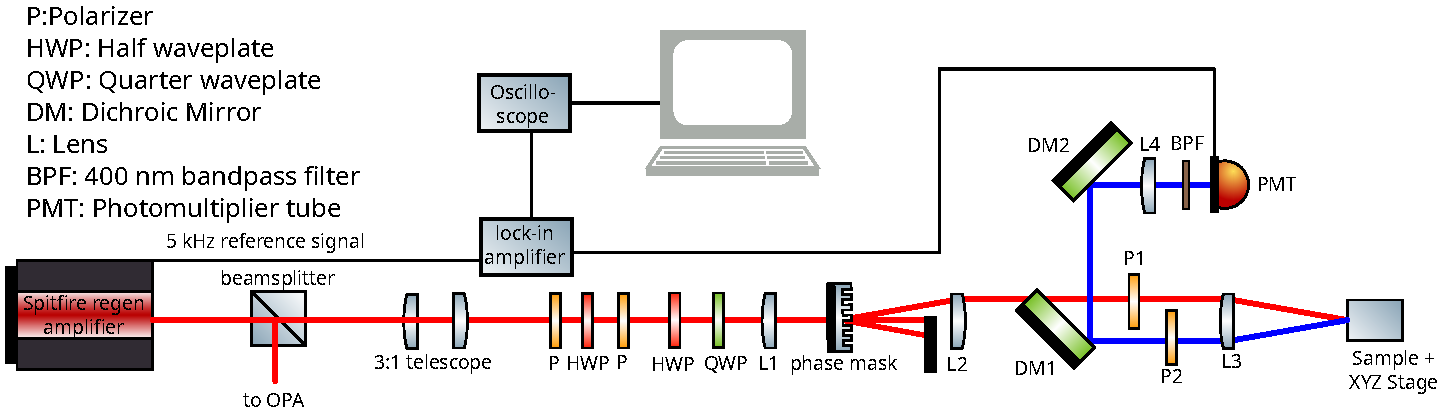
\includegraphics[width=\textwidth]{gfx/ch3/pdf/setup.pdf}
\caption{\label{fig:setup}Schematic drawing of the \gls{shg} setup used in this research. After \citet{morey_automated_2024}.}
\end{figure}

Finally, the polarized output reflects off of two dichroic mirrors (oriented in such a way as to cancel the differing effect of the Fresnel equations on the reflectivity of S and P polarized light) and is focused through a $400$ \si{nm} bandpass filter onto a \gls{pmt} by a $400$ \si{mm} lens.
The current output of the \gls{pmt} is filtered by a lock-in amplifier (for static \gls{shg}, set to the $5$ \si{kHz} repetition rate of the laser) and read out on an oscilloscope.
The phase mask, incoming polarizer, and outgoing polarizer are mounted on rotating lens tubes which are connected via pulley to a common motor shaft driven by a brushless DC motor.
The motor thus continuously rotates the plane of incidence of the experiment, since the latter is entirely defined by the phase mask and the polarizers.
The rotation angle is tracked as a function of time by an optical rotary encoder, consisting of a laser pointer passed through a chopper wheel (with 100 slots) mounted at the end of the motor shaft and detected via photodiode.
The encoder signal and the lock-in signal are both sent to a homemade oscilloscope (an Arduino Uno microcontroller which separates the lock-in signal into different individual rotations by looking for peaks in the encoder signal), the output of which is sent to a computer for further data processing.

\section{Before you build}\label{sec:beforeyoubuild}

I list here a few essential aspects of \gls{shg} that should be considered before designing a new setup.

\subsection{Spot size}

One of the most important quantities in an \gls{shg} setup is the diameter of the probe spot.
Ideally, this diameter is as small as possible, so as to measure the smallest samples or domain sizes.
However, there is an important caveat: for constant fluence (i.e. supposing we are limited by the sample damage threshold), the \gls{shg} signal to noise ratio scales linearly in the area excited by the probe, and thus \gls{shg} microscopes have a difficult time measuring small \gls{shg} signals compared to traditional \gls{shg} setups with a larger excitation area.
To see this, let us say that our detector measures the number of photons per \gls{shg} pulse, which is proportional to the pulse energy $U_p(2\omega)$.
Assuming the input and output pulse intensity profiles have the shape of a square wave with width $\tau$ and height $I_p(\omega)$ and $I_p(2\omega)$, respectively, we have
\begin{equation}
U_p(2\omega) = A I_p(2\omega) \tau
\end{equation}
and
\begin{equation}
U_p(\omega) = A I_p(\omega) \tau
\end{equation}
where $A$ is the area of the beam at the sample surface.
The \gls{shg} intensity is proportional to the square of the input intensity
\begin{equation}
I_p(2\omega) \propto I_p^2(\omega)
\end{equation}
so that
\begin{equation}
U_p(2\omega) \propto \frac{U_p^2(\omega)}{A\tau}.
\end{equation}
Substituting for the fluence $f$
\begin{equation}
f(\omega) = \frac{U_p(\omega)}{A}
\end{equation}
we have
\begin{equation}
U_p(2\omega) \propto \frac{f^2(\omega)A}{\tau}
\end{equation}
i.e., if we hold the fluence constant at the sample damage threshold, the number of photons in the generated \gls{shg} pulse is proportional to the excitation area and inverse to the pulse width.
The signal to noise ratio is then given by
\begin{equation}
\mathrm{SNR} \propto \frac{U_p(2\omega)}{\sqrt{r}}
\end{equation}
where $r$ is the system repetition rate.

\subsection{Oblique vs. normal incidence}

While all of the results presented in this thesis utilized the setup in \cref{fig:setup}, where the incident beam makes a small angle with respect to the sample normal, plenty of groups use a different approach where that angle is set to $0^\circ$.
This has the obvious disadvantage of not specifying all of the tensor elements, since any element $\chi_{ijk}$ with $i, j, k = z$ is not accessible in this geometry.
However, in some cases this can actually be something of an advantage.
For example, sometimes unwanted \gls{shg} contributions (see \cref{sec:manyshgterms}) may be avoided in the normal incidence geometry, assuming the \gls{na} of the focusing optic is small enough that longitudinal components of the electric field are nearly zero.
Furthermore, in some materials the order parameter only couples to one or two elements of $\chi_{ijk}$; if none of these elements have a $z$ index, it is needless to complicate the analysis with oblique incidence.

In my experience, oblique incidence seems to be useful in two broad cases.
For one thing, some order parameters only show up in the $z$ components of $\chi_{ijk}$ (this is the case in \tastwo, see \cref{sec:tastwo}), in which case one obviously needs a nonzero angle of incidence to access these components.
A more subtle point is that, even if in practice all of the phenomenology of a particular sample only shows up in the $x$ and $y$ indices of $\chi_{ijk}$, still one must measure the full tensor to \emph{rule out} unseen phenomenology in the other indices.
Both the \ce{CaMn2Bi2} (\cref{ch:ch5}) and \ce{CuBr2} (\cref{ch:ch6}) works presented in this thesis are examples of exactly this point, where the main scientific arguments involve either comparing \gls{shg} patterns in two domains or comparing oscillation amplitudes in different polarization channels.
Clearly one needs to know all of the tensor elements to make those arguments exact.

\chapter{Automated polarization rotation for multi-axis RA-SHG experiments}\label{ch:polrotators}
\chaptermark{Automated polarization rotation}
\section{Preface}

This chapter is based on a manuscript intended for standalone publication and modified to fit the format of this thesis.
It was coauthored by myself and Karna Morey (as co-first authors), along with Baiqing Lv, Zongqi Shen, and Nuh Gedik.
Karna Morey and I initiated the project, designed and built the polarization rotators, performed the demonstration experiment, and wrote the paper.
Baiqing Lv and Zongqi Shen contributed to the design and helped review the manuscript.
Nuh Gedik supervised the project.

\section{Abstract}

\gls{rashg} is a nonlinear optical technique used to probe the symmetry of condensed matter systems. 
Measuring the dependence of the SHG susceptibility on one or more external parameters, notably strain, field, temperature, or time delay, is an extremely powerful way to probe complex phases of quantum materials. 
Experimentally, extracting maximal information about the SHG susceptibility tensor requires measurements of S and P polarized input and output combinations, which naturally involves the rotation of the polarizers during data collection.  
For multi-axis experiments, this has proved challenging since polarization rotation is typically done manually. 
Automating this process eliminates labor constraints, reduces uncertainty due to low-frequency noise, and expands the type of multi-axis datasets that can be collected; however, it is difficult due to geometrical constraints within the setup.
In this work, we design and implement low-cost, high-fidelity automated polarization rotators for use in multi-axis \gls{rashg}.
These polarization rotators utilize an electrical slip ring to transfer power to the rotating \gls{rashg} optical setup as well as a miniature stepper motor to perform the polarization rotation.
We demonstrate this automated system in time-resolved \gls{rashg} measurements in the non-centrosymmetric semiconductor \ce{GaAs}. 
For the multi-axis measurements described above, this automated system permits data averaging over longer periods, vastly expedites data collection, and expands the setup measurement capability.
This ultimately opens new frontiers in probing quantum materials using multiple tunable external parameters.

\section{\label{km-sec:intro} Introduction}

Probing the structure of crystalline solids is essential to understanding their intrinsic functionalities. 
Traditionally, diffraction techniques based on the scattering of e.g. x-rays are used to determine this structure; however, these techniques predominantly measure the total electron density and are thus insensitive to long-range ordering of the valence electron subsystem.
In contrast, nonlinear scattering techniques at optical frequencies like \gls{rashg} are sensitive rather to the total charge density, and thus offer a complementary view of the electronic, magnetic, and lattice properties of quantum materials \citep{torchinsky_low_2014, fichera_second_2020}.\footnote{In this paper, we discuss \glsfmtshort{rashg}, although the results are fully generalizable to arbitrary harmonics, e.g. third harmonic generation.}


Furthermore, due to the non-invasive nature of \gls{rashg}, it can also be used to investigate changes along one or more measurement axes, such as strain, field, pressure, temperature, or time delay.
The phase diagram of quantum materials is heavily influenced by these independent variables, and thus, changes to the SHG response along such measurement axes are of great interest.
For example, previous studies have used various continuous experimental parameters such as pressure \citep{li_high-pressure_2022}, time delay\citep{shan_giant_2021}, and magnetic field to investigate phase transitions in quantum materials.
Such measurements can illuminate the roles that charge, spin, and thermal degrees of freedom play within quantum materials.

Second harmonic generation gleans microscopic information through the coupling of an order parameter to the second harmonic susceptibility tensor (at least a third-rank tensor with 18 independent components) \citep{boyd}. 
This tensor governs the relationship between the vector properties (i.e. polarization and intensity) of the incident radiation and the generated second harmonic, as shown in \cref{km-eq:intensity}.
The complexity of this tensor means that a significant amount of data is needed to fully resolve the tensor components, posing experimental challenges with data collection.
The importance of resolving the tensor components can be seen by considering Neumann's principle, which states that these tensors must be invariant under symmetry operations of the material's point group, which constrains the tensors' independent and nonzero elements \citep{birss}. 
By measuring the intensity and polarization of the generated second harmonic radiation, \gls{rashg} provides information about these tensor elements and thus the underlying point group.
When performing experiments with more than one measurement axis, the data constraints mentioned above can often be especially burdensome, limiting the type of experiments that can be performed using \gls{rashg}.
Thus, new methods for collecting data efficiently for multi-axis \gls{rashg} experiments are incredibly important.

\begin{figure}
\centering
\phantomsubfloat{\label{km-fig:1a}}
\phantomsubfloat{\label{km-fig:1b}}
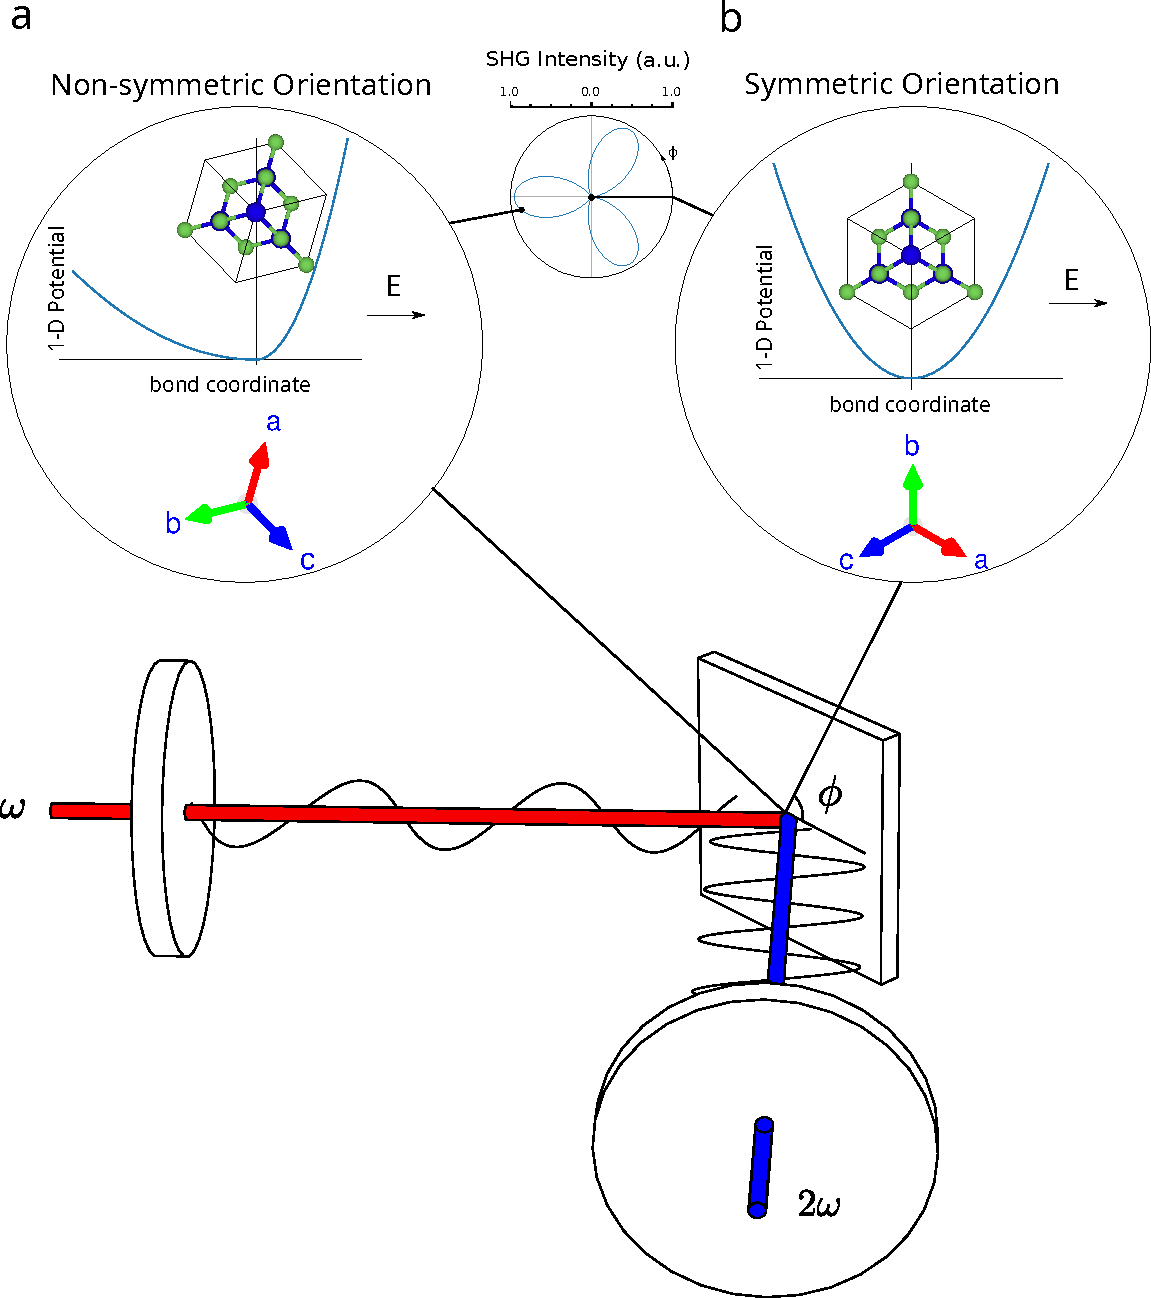
\includegraphics[width=0.8\textwidth]{gfx/ch4/km-fig1.pdf}
\caption[A demonstration of \glsfmtshort{rashg} in the test sample \ce{GaAs}]{
\label{km-fig:1}
\begin{enumerate*}[label=\caplabel, ref=\capref]
\item[] A demonstration of \glsfmtshort{rashg} in the test sample \ce{GaAs}.
\qty{800}{nm} light comes in at an oblique angle of incidence, after being passed through a polarizer.
The polarization axis of the light is in the plane of incidence and is denoted in the insets of the figure with a black arrow.
Depending on the angle of the plane of incidence relative to the crystallographic axes, as well as the polarization of the beam relative to that incoming plane of incidence, the second harmonic response to the stimuli should vary from zero points (nodes) to non-zero maxima.
\end{enumerate*}
}
\end{figure}

A more detailed understanding of the information that needs to be collected to fully resolve the second harmonic susceptibility can be seen by considering \cref{km-fig:1}.
\Cref{km-fig:1} shows a schematic of an \gls{rashg} setup, where near-infrared light from the laser source enters at oblique incidence and is scattered off the front of the sample, generating blue light at the second harmonic frequency.
To leading order, the measured second harmonic intensity is given by
\begin{equation}
I(\phi) = \big| E^{\mathrm{out}}_i(\phi) \chi^{(2)eee}_{ijk} E^{\mathrm{in}}_j(\phi) E^{\mathrm{in}}_k(\phi)\big|^2,
    \label{km-eq:intensity}
\end{equation}
where $\phi$ is the azimuthal angle between the crystallographic axes and the plane of incidence, $E^{\mathrm{out}}$ and $E^{\mathrm{in}}$ are the polarization vectors of the outgoing and incoming light, respectively, and $\chi^{(2)eee}$ is the SHG electric-dipole susceptibility tensor.
For certain values of $\phi$, as shown in \cref{km-fig:1a}, the sample is symmetric with respect to the polarization axis of the incoming light; in this case, the second harmonic generation is constrained to be zero, whereas in general arbitrary angles give a non-zero second-harmonic response (see \cref{km-fig:1b}).
Neumann's principle dictates that \cref{km-eq:intensity} captures the symmetry considerations shown in \cref{km-fig:1}, i.e. the symmetries of the crystal are embedded into its nonlinear susceptibility tensor $\chi^{(2)}$.

These considerations demonstrate the necessity of measuring the full rotational anisotropy of the SHG response, as well as its dependence on the incoming and outgoing polarization directions (which may be P or S-polarized, leading to four independent polarization channels).
The former requires rotating the plane of incidence, which is typically done by rotating the optical setup itself rather than the sample \citep{petersen_nonlinear_2006,torchinsky_low_2014, fichera_second_2020, camn2bi2}. 
The geometric constraints involved in rotating the optical setup make it challenging to use electromechanical components to rotate the polarizers shown in \cref{km-fig:1} between S and P configurations, since naively it is difficult to transfer power to the rotating frame of reference.
Because of this, switching between different polarization channels is typically done manually, resulting in time and labor constraints that often limit data collection beyond a single polarization combination \citep{shan_giant_2021}.
Such constraints severely restrict the ability to infer tensor elements from the \gls{rashg} data and limit RA-SHG to studies involving often just a single tuning parameter. 

Previous multi-axis \gls{rashg} studies typically either collected exclusively one polarization channel \citep{shan_giant_2021} (for more than one axis) or simply sacrificed the quantity of collected data and therefore inferred statistics. 
However, these approaches can often miss certain features in \gls{rashg} data that would be apparent if more efficient data-taking methods were available.
For example, phase transitions in which the order parameter couples differently to different polarization channels through the second harmonic susceptibility \citep{camn2bi2} are best characterized by taking the full rotational anisotropy data.
The benefit of collecting all four polarization combinations underscores the appeal of automated polarization control of \gls{rashg} setups.

\begin{figure}
\centering
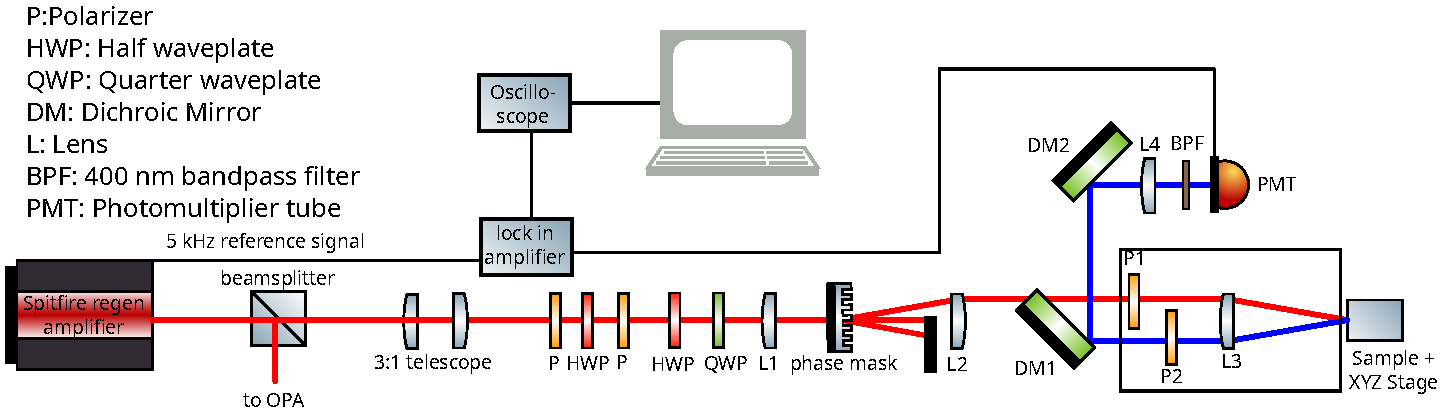
\includegraphics[width=\textwidth]{gfx/ch4/km-fig2.pdf}
\caption[A diagram of the full second harmonic generation setup]{
\label{km-fig:2}
\begin{enumerate*}[label=\caplabel, ref=\capref]
\item[] A diagram of the full second harmonic generation setup developed and described in \citet{fichera_second_2020}.
Boxed in part of the setup shows the area of interest of this work, where the incoming and outgoing polarization channels are set.
\end{enumerate*}
}
\end{figure}

In this work, we design and implement automated polarization rotators for use in multi-axis \gls{rashg} measurements. 
The devices utilize a miniature stepper motor housed in an electrical slip ring to circumvent the geometrical constraints imposed by the rotating plane of incidence.
In section \ref{km-sec:disc}, we discuss the specific application of automated polarization rotation to time-resolved RA-SHG and show that it not only expedites data collection but also reduces the setup's sensitivity to low-frequency noise. 
The advantages afforded by the automated polarization rotators exist not only for time-resolved measurements but for any measurements where an external parameter is being varied and compound rapidly as multiple parameters are varied at the same time.

\section{Design}
\label{sec:des}

A detailed schematic of the \gls{rashg} setup is shown in figure 2.
Telescoped pulses from a \qty{5}{kHz} pulsed regenerative amplifier (Spectra-Physics Spitfire) are attenuated using a half-waveplate set between two polarizers and then elliptically polarized using a half-waveplate and quarter-waveplate in series. 
The light is then focused by a lens onto a rotating phase mask (which separates the beam into different diffraction orders), and a beam block selects the +1 order beam which is then collimated using another lens (L2).
Finally, the beam passes through a dichroic mirror and a polarizer (P1) before being focused by a third lens (L3) onto the sample.
The reflected radiation is passed through an analyzer (P2) and is redirected using a dichroic mirror periscope, which has equal reflectivity for S and P-polarized light and selects exclusively the \qty{400}{nm} reflected radiation.
The two polarizers (P1 and P2) and the phase mask are mounted on a rotating shaft coupled to an optical rotary encoder.
After the dichroic mirrors, the second harmonic radiation is focused by a final lens (L4) onto a \qty{400}{nm} bandpass filter and photomultiplier tube.
The signal from the photomultiplier tube is sent to a lock-in amplifier synced to the \qty{5}{kHz} pulsed laser reference signal and the amplified signal is then correlated with the signal from the optical rotary encoder using a home-built oscilloscope. 

Importantly, the geometrical constraints introduced by the rotating plane of incidence mean that rotating P1 and P2 between S and P configurations electromechanically is challenging, as power must be transmitted from the stationary laboratory frame to electrical components lying in the rotating frame.

To solve this problem, we utilize a hollow-bore electrical slip ring and a miniature stepper motor, shown in an exploded-view diagram in \cref{km-fig:3a}.
A slip ring uses stationary conductive brushes sliding against a rotating through-bore cylinder to transfer power from a stationary reference frame to a rotating one, as shown in \cref{km-fig:3b} \citep{argibay_asymmetric_2010}. 
To accommodate the further requirement that the beams pass through the entire device unimpeded, we employ an \qty{8}{mm} stepper motor that fits in between the two beams.
\Cref{km-fig:3c} and \cref{km-fig:3d} show a front view of the device, with the wire grid polarizer in the P and S positions, respectively, and the polarization direction of the polarizer shown in arrows on the edge of the polarizer.
A full rendering, to scale, of the automated system within the full setup is shown in \cref{km-fig:6}. 

\subsection{Slip Ring}

Slip rings are a standard electromechanical device for transferring power from a stationary assembly to a rotating assembly.
An inner, rotating part of the slip ring can freely rotate relative to an outer, stationary part without compromising signal or power transmission.
This functionality is enabled by low-friction metal brushes that slide against another set of electrical contacts, allowing free rotation while maintaining good electrical conductivity \citep{argibay_asymmetric_2010}, as shown in \cref{km-fig:3b}.
To allow for the uninterrupted passage of the beams through the device, we use a hollow-bore slip ring (Moflon MT3899-S040-VD) whose \qty{38}{mm} inner bore rotates along with the lens tube-pulley assembly shown in \cref{km-fig:6}.
Either set screws located on the front side of the slip ring (as shown in \cref{km-fig:3}) or a 3D-printed cylindrical hollow bore adapter (not shown) can secure the inner bore of the slip ring to the lens tube.

\begin{figure}
\centering
\phantomsubfloat{\label{km-fig:3a}}
\phantomsubfloat{\label{km-fig:3b}}
\phantomsubfloat{\label{km-fig:3c}}
\phantomsubfloat{\label{km-fig:3d}}
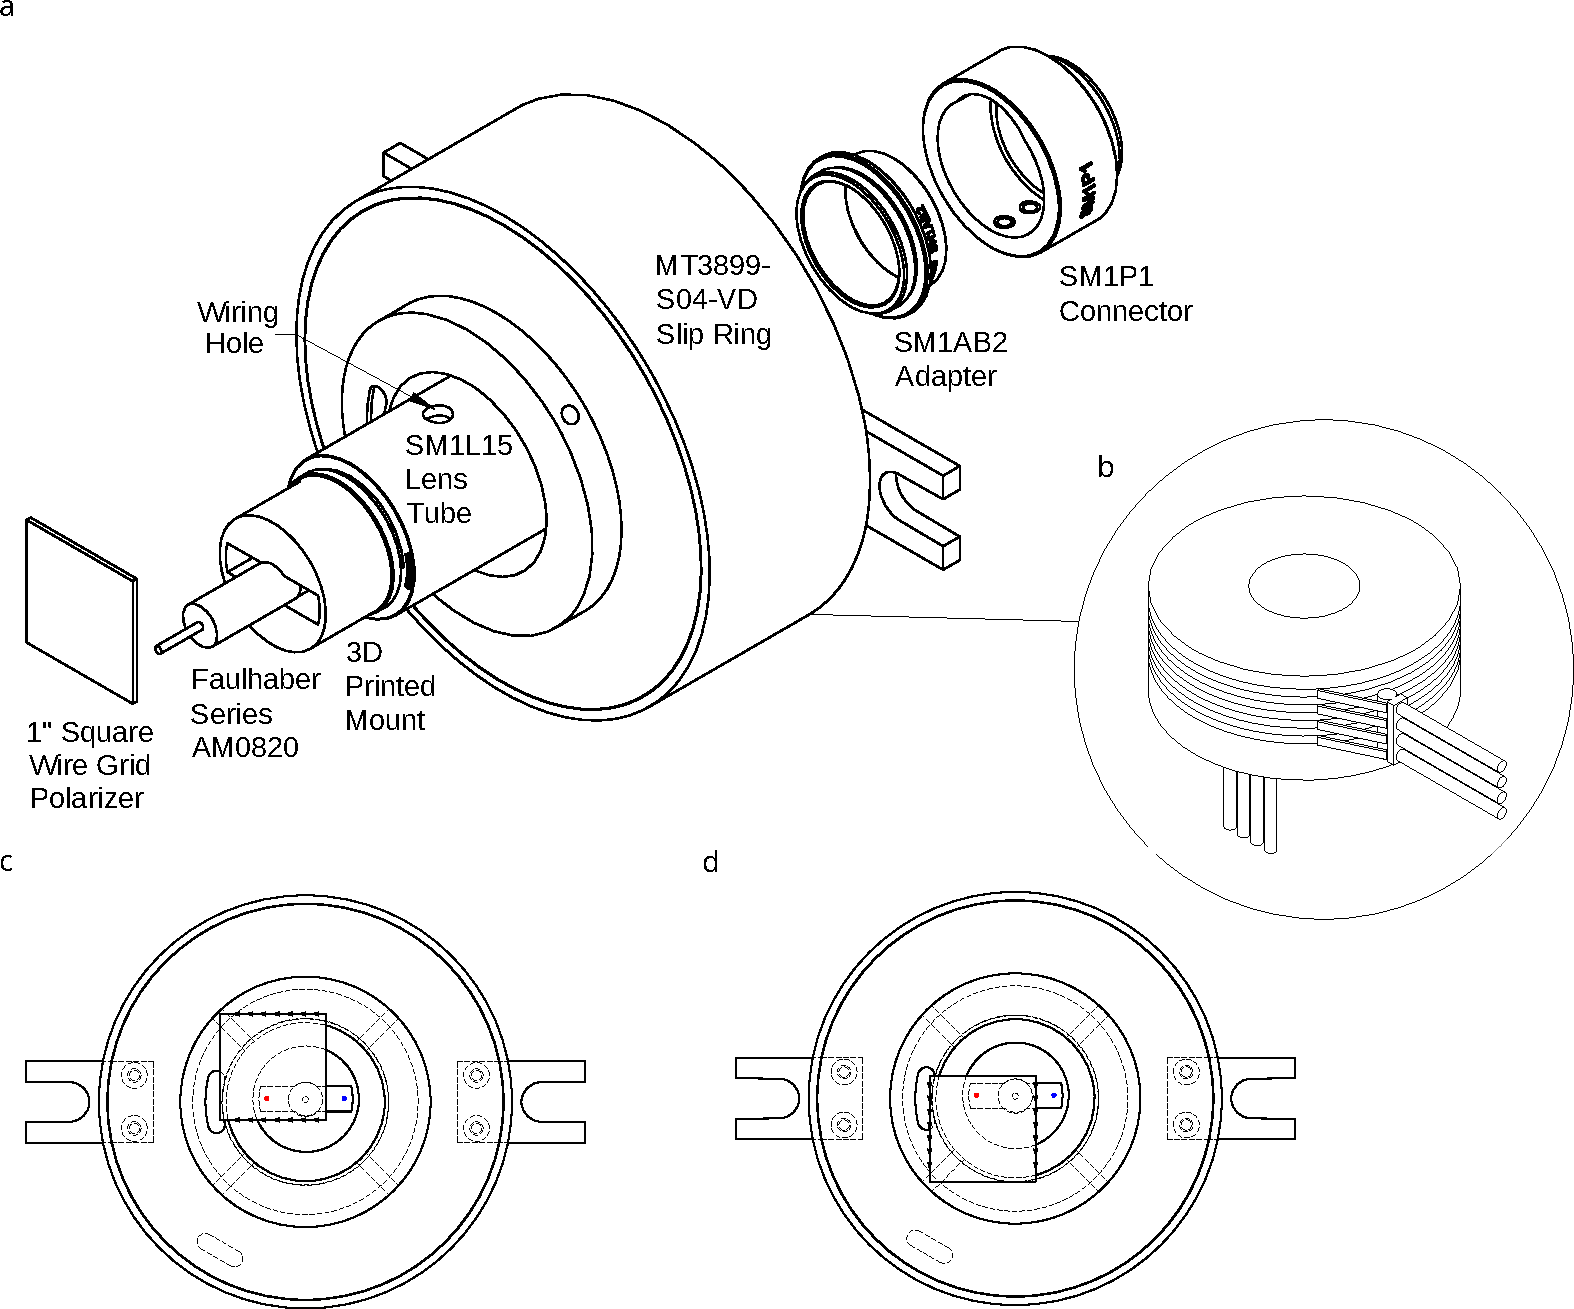
\includegraphics[width=\textwidth]{gfx/ch4/km-fig3.pdf}
\caption[Exploded-view diagram of one of the automated polarization rotators]{
\label{km-fig:3}
\begin{enumerate*}[label=\caplabel, ref=\capref]
\item An exploded-view diagram of one of the automated polarization rotators, with the individual components labeled.
Each of these is a manufactured part except for the 3D-printed mount.
\item A schematic of the interior of an electrical slip ring, where low-friction metal brushes allow for electrical conduction across a rotating assembly.
\item A front view of the device, in the P-polarized state, with arrows on the edge of the polarizer indicating the polarization direction.
\item Same as \cref{km-fig:3c}, but in the S-polarized state.
\end{enumerate*}
}
\end{figure}

\subsection{Miniature Stepper Motor}
\label{km-sec:stepper}
The hollow bore slip ring allows for the transfer of power to the rotating shaft.
To rotate the wire grid polarizer between S and P configurations while also allowing both beams to pass through the entire device, we use an \qty{8}{mm} diameter Faulhaber Series AM0820 stepper motor.
The stepper motor's shaft is epoxied to a \qty{1}{inch} square wire-grid polarizer roughly \qty{5}{mm} from the closest horizontal and vertical edges, as shown in \cref{km-fig:3c} and \cref{km-fig:3d}.
The stepper motor is mounted in the center of the SM1L15 lens tube using a custom, 3D printed mount as shown in \cref{km-fig:3a}. 
This mount, along with careful epoxying of the polarizer to the motor shaft, ensures that the incidence angle of the beam is close to normal.
Furthermore, the mount ensures that the stepper motor's shaft is aligned closely to the central rotation axis of the entire assembly, minimizing torques on the motor and polarizer.
This stepper motor can support up to \num{800} total micro-steps per revolution (\ang{0.45} per micro-step) and \qty{0.65}{mNm} of holding torque, and is small enough to fit in between the incoming and outgoing beams. 

The motor can then move the polarizer between the P configuration (\cref{km-fig:3c}) and the S configuration (\cref{km-fig:3d}) without manual intervention or the need to stop the rotation of the entire assembly.
The offset placement of the polarizer on the motor shaft allows only one of the beams (either incoming or outgoing) to pass through the polarizer.
The SM1AB2 and SM1P1 adapter pieces allow for arbitrary rotation relative to the longer lens tube-pulley assembly, allowing the beams to be aligned with the empty spaces in the stepper motor mount.
These adapter pieces also allow for small ($\pm \ang{20}$) rotations of the polarizer about the central axis to account for factory defects which may cause the polarization axis to be misaligned with the straight edges of the polarizer.

\begin{figure}
\centering
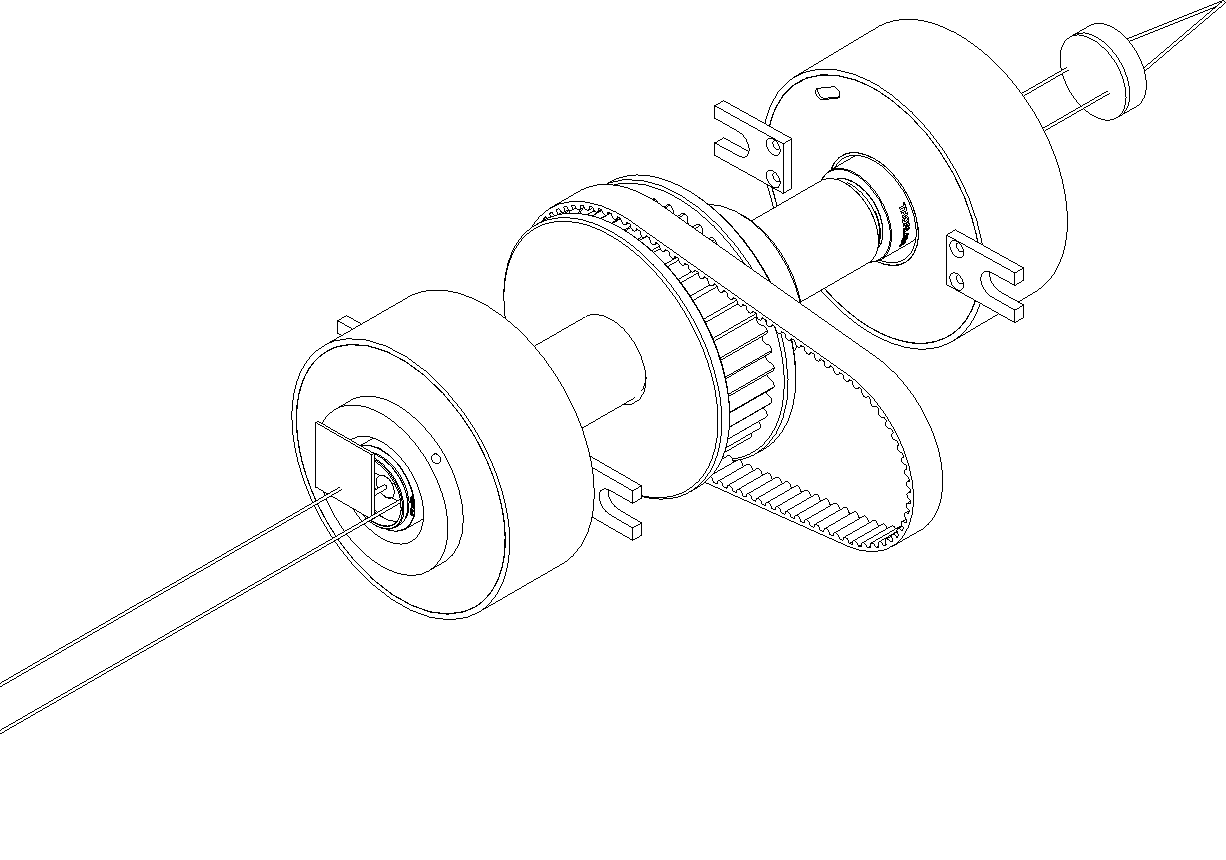
\includegraphics[width=\textwidth]{gfx/ch4/km-fig4.pdf}
\caption[A 3-dimensional rendering of the automated polarization rotators]{
\label{km-fig:6}
\begin{enumerate*}[label=\caplabel, ref=\capref]
\item[] A 3-dimensional rendering of the boxed-in part of the setup in \cref{km-fig:2}, with fully automated polarization rotators.
\end{enumerate*}
}
\end{figure}

Another copy of the same system shown in \cref{km-fig:3} is mounted on the other side of the lens tube-pulley assembly and controls the polarization of the reflected beam, as shown in \cref{km-fig:6}. 
The back sides of both devices, shown in \cref{km-fig:6}, are attached to the rotating lens tube-pulley-motor-shaft assembly shown in \cref{km-fig:6} via threads on the long central lens tube. 
A hole drilled in the top and bottom of the SM1L15 piece in each device shown in figure \cref{km-fig:3a} allows feedthrough wires to connect the four leads of the stepper motor to the four rotating inner-bore slip ring leads.
The four leads on the stationary side of each slip ring directly connect to a Geckodrive G250X digital step driver for each device, controlled by a single Arduino Nano Every.
This control circuit allows for the integration of the stepper motors with existing instrumentation software.

Whenever the stepper motors lose power, the polarizers need to be re-aligned due to the loss of their holding torque.
The alignment is performed by using a reference polarizer with a known polarization axis.
First, the plane of incidence of the entire assembly is positioned to the known polarization plane of the reference polarizer, then the polarizers themselves can be oriented by placing the beam through the reference polarizer and rotating the stepper motor until beam extinction (yielding an S-polarized alignment).  
The polarizers can then freely rotate between this S-polarized position and the orthogonal P-polarized position.

\section{Validation and Discussion}
\label{km-sec:disc}

\begin{figure}
\centering
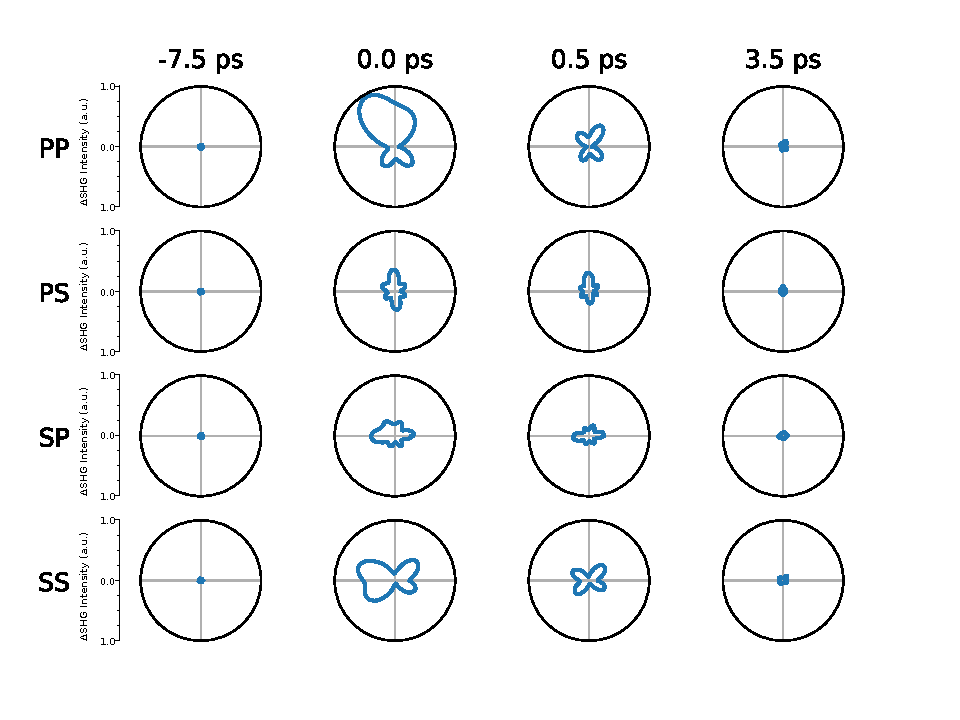
\includegraphics[width=\textwidth]{gfx/ch4/km-fig5.pdf}
\caption[Demonstration of the automatic polarization rotators]{
\label{km-fig:4}
\begin{enumerate*}[label=\caplabel, ref=\capref]
\item[] A polar plot of the change in SHG intensity (from the pre-pump state) as a function of time since zero-delay for the test sample GaAs.
This is a demonstration of using the automated polarization rotators to take \gls{trshg} data.
\qty{55} different pump-probe delays (only four time delays are plotted) were taken in this dataset, meaning that \qty{220} polarization rotations were performed using the automated polarizers.
\end{enumerate*}
}
\end{figure}

To test these automated polarization rotators, we performed time-resolved RA-SHG on the non-centrosymmetric semiconductor \ce{GaAs} \citep{ducuing_observation_1963, torchinsky_low_2014}. 
A pump line was added to the setup shown in \cref{km-fig:2} by mounting a \ang{45} mirror onto L3 so that the pump beam may be reflected directly onto the sample. 
The pump pulse is produced by an optical parametric amplifier (Spectra-Physics Topas) tuned to a wavelength of \qty{1.3}{$\mu$ m}.
The pump line includes a delay stage, which controls the relative time delay between the pump and the probe pulses, and a chopper wheel, which reduces the effective repetition rate of the pump pulses to \qty{2.5}{kHz}. 
With the pump repetition rate of \qty{2.5}{kHz} and the probe repetition rate of \qty{5}{kHz}, locking in at a frequency of \qty{2.5}{kHz} produces a signal proportional to the change in the \gls{shg} intensity relative to equilibrium.
For time-resolved measurements on \ce{GaAs}, shown in \cref{km-fig:4}, \qty{55} different pump-probe delays were taken, resulting in \qty{220} different automatic rotations of the polarizers.
The data in \cref{km-fig:4} shows the change in the \gls{shg} intensity relative to equilibrium as a function of the pump-probe delay, for each of the polarization channels. 
The use of the polarization rotators in this validation measurement demonstrates their functionality and broad utility for multi-axis \gls{rashg} measurements.

This system was also used to expedite data collection in recent studies of time-resolved, temperature-dependent \gls{rashg} \citep{camn2bi2}.
This particular type of \gls{rashg} measurement demonstrates the general advantages of automated polarization control in multi-axis \gls{rashg} measurements.
To see this, note that if the rotation of the polarizers is performed manually, the best data-taking strategy involves taking the time dependence of one polarization channel in full before moving to the next. 
However, in the presence of low-frequency noise (due to e.g. fluctuations in the laser intensity), this is problematic as the different polarization channels will not be taken under equivalent conditions. 
In the automated case, in contrast, all polarization channels can be taken at each time delay. 
This greatly decreases the experiment's susceptibility to low-frequency noise and expedites data taking by allowing for overnight and multi-day scans.

Automated polarization rotation thus vastly improves RA-SHG data collection, eliminating the need for manual polarization rotation, especially in cases of multiple experimental axes. 
The roughly \qty{1,000}{\$} total cost of both devices (not including polarizers) makes them relatively inexpensive, and the design is easily implementable in existing \gls{rashg} setups.
Multi-axis measurements are becoming increasingly important to resolve complicated phase diagrams and competing orders, and thus future measurements will increasingly rely on automated systems such as the one presented in this work.

\chapter{Second harmonic generation as a probe of broken mirror symmetry in \tastwo}\label{ch:tastwo}
\chaptermark{SHG as a probe of broken mirror symmetry in \tastwo}
\section{Preface}

This chapter is based on a manuscript that was published as a Rapid Communication in \textit{Physical Review B} in 2020, again modified to fit the format of this thesis.
It was coauthored by myself, Anshul Kogar, Linda Ye, Bilal G\''okce, Alfred Zong, Joseph G. Checkelsky, and Nuh Gedik.
Anshul Kogar and I initiated the project and took the \gls{rashg} data.
Linda Ye and Joseph G. Checkelsky grew the samples, Bilal G\''oke helped build the \gls{rashg} setup, and Alfred Zong took some \gls{ued} data.
I analyzed the data and wrote the paper.
Nuh Gedik supervised the project.

\section{Abstract}

The notion of spontaneous symmetry breaking has been used to describe phase transitions in a variety of physical systems.
In crystalline solids, the breaking of certain symmetries, such as mirror symmetry, is difficult to detect unambiguously.
Using \tastwo, we demonstrate here that rotational-anisotropy second harmonic generation (RA-SHG) is not only a sensitive technique for the detection of broken mirror symmetry, but also that it can differentiate between mirror symmetry-broken structures of opposite planar chirality.
We also show that our analysis is applicable to a wide class of different materials with mirror symmetry-breaking transitions.
Lastly, we find evidence for bulk mirror symmetry-breaking in the incommensurate charge density wave phase of \tastwo.
Our results pave the way for RA-SHG to probe candidate materials where broken mirror symmetry may play a pivotal role.

\section{Introduction}

In condensed matter systems, phases are often classified by the symmetries that they break.
Identifying these symmetries enables one to understand a system's order parameter, collective excitations, topological defects, and allowable topological indices \cite{sethna, thouless}.
Together, these attributes allow one to predict how a material will respond to external perturbations like electromagnetic fields, heat, and mechanical forces, which is a central goal of condensed matter physics.

Specifically, the presence or absence of mirror symmetry can lead to a variety of unusual phases and properties.
For example, the absence of mirror plane symmetry in noncentrosymmetric materials can give rise to gyrotropic order, which can lead to a nonzero out-of-plane circular photo-galvanic effect \cite{belinicher1980}.
Moreover, in certain topological crystalline insulators, such as SnTe, the presence of mirror symmetry can give rise to conducting surface states through the existence of a nonzero mirror Chern number.
This topological index guarantees an even number of Dirac cones on surfaces where mirror symmetry is retained \cite{teo2008, hsieh_topological_2012, fu_topological_2011}.

In other circumstances, like that in the pseudogap regime of cuprate superconductors, the existence of mirror symmetry is more controversial and has led some to seek an experimental method to serve as a binary indicator of broken mirror symmetry \cite{hlobil_elastoconductivity_2015}.
In principle, several tools can already do this, including resonant ultrasound spectroscopy \cite{leisure1997, migliori1993}, X-ray, neutron, and electron diffraction \cite{bacon1966, dorset2013}, and a recently-proposed method, shear conductivity \cite{hlobil_elastoconductivity_2015}.
Resonant ultrasound spectroscopy and the diffraction-based techniques are more sensitive to the ionic lattice, which makes the identification of subtle electronic symmetry-breaking challenging.
And while shear conductivity has the potential to be an extremely versatile tool for identifying broken point group symmetries, experimental pursuits are currently only preliminary \cite{hlobil_elastoconductivity_2015}.
In this study, we focus on a nonlinear optical technique, rotational-anisotropy second harmonic generation (RA-SHG), which we show is capable not only of identifying broken mirror symmetry \cite{heinz_study_1985} but also of resolving its sense (left- or right-handed).
Furthermore, RA-SHG is sensitive to the electronic subsystem and can be used for microscopy studies, making it an ideal experimental tool for probing phase transitions where domains may arise \cite{kumar_magnetic_2017, harter_parity-breaking_2017}.

In this direction, we choose a material, \tastwo, in which vertical mirror plane symmetry is manifestly broken across an incommensurate (IC) to nearly commensurate (NC) charge density wave (CDW) transition \cite{wilson_charge-density_1975, zong_ultrafast_2018}.
Using this material, we demonstrate in this Rapid Communication that RA-SHG is an effective probe of broken mirror symmetry.
We also show that the sense (i.e. left- or right-handed) associated with the mirror symmetry-broken structure is encoded in the angular dependence of the RA-SHG signal.
Thus, RA-SHG can be used to differentiate mirror-opposite domains. 
While the data presented in this work is specific to the case of \tastwo, we also show analytically that our technique is applicable to a wide class of transitions involving spontaneously broken mirror symmetry.

\tastwo is a layered material with a crystallographic structure identical to other octahedrally-coordinated transition metal dichalcogenides (Fig.~\ref{fig:fig0}(a)).
The space group of the high temperature, undistorted phase is $P\bar{3}m1$ (no.164, point group $D_{3d}$)~\cite{spijkerman_x-ray_1997}, and the point group of the surface normal to the (001) direction in this phase is $C_{3v}$~\cite{scruby_role_1975, fung_application_1980}.
Upon lowering temperature, \tastwo undergoes a series of CDW transitions.
At $T_{\mathrm{IC}}=\qty{550}{K}$, a triple-$q$ IC CDW forms which breaks translational symmetry but retains the surface point group symmetries of the undistorted phase~\cite{scruby_role_1975, fung_application_1980}.
The effects of the CDW on the bulk symmetries in this phase are not yet understood.
On further cooling, at $T_{\mathrm{IC-NC}}=\qty{353}{K}$ there is a weak first-order transition to an NC CDW phase where three vertical mirror plane symmetries are broken~\cite{spijkerman_x-ray_1997} and the surface point group becomes $C_3$.
The NC phase has been visualized with scanning tunneling microscopy and exhibits patches of commensurate ``Star of David" hexagrams that are separated by a network of discommensurations \cite{wu_hexagonal_1989}.
Because mirror symmetry is broken, there are two energetically equivalent CDW configurations ($\alpha$ and $\beta$) in the NC phase that have opposite planar chirality (Fig.~\ref{fig:fig0}(c)-(d)).
At even lower temperatures, $T_{\mathrm{NC-C}}=\qty{184}{K}$, \tastwo undergoes a symmetry-preserving first-order transition, where the discommensurations disappear and the CDW locks into a structure commensurate with the underlying lattice~\cite{ishiguro_high-resolution_1995}.

\begin{figure}
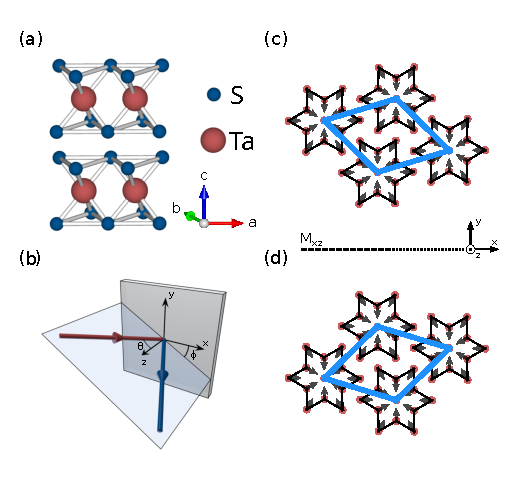
\includegraphics{fig0red1.pdf}%
\caption{\label{fig:fig0}
(a) Structure of \tastwo in the undistorted phase. 
Ta and S atoms are depicted in red and blue, respectively. 
(b) Schematic of the experimental geometry.
(c-d) Structure of the CDW in the NC phase.
Arrows denote the movement of the Ta atoms (red) below $T_\mathrm{IC-NC}=\qty{353}{K}$ from their undistorted positions.
The transition at $T_{\mathrm{IC-NC}}$ spontaneously breaks mirror symmetry, so that two different CDW configurations ($\alpha$ and $\beta$) can form which have opposite planar chirality.
The new unit cells of the two configurations are depicted in blue.
$M_{xz}$ denotes one vertical mirror plane which is broken beneath $T_\mathrm{IC-NC}$.
The others are related to $M_{xz}$ by $\pm \ang{120}$ rotation about the $z$ axis.}
\end{figure}

Recent interest in the NC phase of \tastwo has arisen due to the possibility of injecting mirror-opposite domains into the CDW structure \cite{zong_ultrafast_2018} which do not otherwise develop during the IC-NC transition.
Zong \textit{et al.} were able to induce these domains using a single ultrafast pulse of light, which was found to drive the material into a long-lived metastable state possessing domains of opposite planar chirality.
Partly motivated by the desire to image these domains, we seek here a simple experimental method that could identify domains with opposite planar chirality.

\section{Results and discussion}

\tastwo samples used in the experiment were grown using the chemical vapor transport technique, as described in Ref.~\cite{zong_ultrafast_2018}.
We verified that the NC phase of \tastwo was single-domain by performing electron diffraction on a sample from the same batch\cite{supplementary_materials}.
This is in agreement with previous works~\cite{zong_ultrafast_2018, wilson_charge-density_1975, bovet_pseudogapped_2004, shiba_phenomenological_1986}.

In RA-SHG~\cite{harter_high-speed_2015, lu_fast_2018, torchinsky_structural_2015, lu_fourier_2018}, a pulsed laser beam of frequency $\omega$ and amplitude $E(\omega)$ is focused onto a sample with nonzero angle of incidence $\theta$ (Fig.~\ref{fig:fig0}(b)).
The $2\omega$ component of the radiation emitted by the sample is subsequently measured in various combinations of incoming and outgoing polarizations (either parallel (P) or perpendicular (S) to the plane of incidence) and as a function of the angle $\phi$ between the plane of incidence and some crystallographic axis.
In noncentrosymmetric materials, the response is dominated by the bulk electric dipole moment $P_i(2\omega) = \chi_{ijk}E_j(\omega)E_k(\omega)$ \cite{boyd}, where $\chi_{ijk}$ is a material-specific susceptibility tensor which must be invariant under all symmetry operations present in the crystallographic point group.
In centrosymmetric crystals such as \tastwo, the bulk electric dipole response is forbidden~\cite{boyd, powell}.
In this case, the dominant response often comes from the surface of the sample, which necessarily breaks inversion symmetry~\cite{bloembergen_optical_1968}.
SHG from surfaces of materials is described by a different susceptibility tensor, $\chi_{ijk}^S$, which is constrained by the crystal symmetries of the surface.
In addition, there can be bulk contributions from higher-order processes which are allowed in the presence of inversion symmetry, such as the bulk quadrupole response $Q_{ij}(2\omega) = \chi^Q_{ijkl}E_k(\omega)E_l(\omega)$~\cite{kumar_magnetic_2017, shen}.
Our experimental implementation uses a fast-rotation setup similar to that described in Refs.~\onlinecite{harter_high-speed_2015} and \onlinecite{torchinsky_low_2014}.
Here, we use an \qty{800}{nm} (\qty{1.55}{eV}) laser beam incident at $\ang{10}$ with respect to the (001) sample normal.
Further experimental details can be found in the supplement\cite{supplementary_materials}.

To show that we are sensitive to the breaking of mirror symmetry across the IC to NC transition, we took RA-SHG data on \tastwo in both phases.
Figs.~\ref{fig:fig1}(a) and \ref{fig:fig1}(b) show the second harmonic response from the sample above and below $T_{\mathrm{IC-NC}} = \qty{353}{K}$ in two polarization channels, plotted as a function of $\phi$.
We are able to fit the rotational anisotropy in the IC phase using the surface point group $C_{3v}$ (Fig.~\ref{fig:fig1}(a)), which is in agreement with previous reports~\cite{scruby_role_1975, fung_application_1980}.
It should be noted that in order to fit the S$_\mathrm{in}$-S$_\mathrm{out}$ polarization channel appropriately, we find that it is necessary to add an additional bulk quadrupole contribution to the signal.
The consequences of this contribution will be discussed later, but at the moment they do not affect our conclusions.

\begin{figure}
\includegraphics{fig2.pdf}
\caption{\label{fig:fig2}Second harmonic intensity as a function of $\phi$ from mirror-opposite samples of \tastwo in the NC phase ($T=\qty{340}{K}$).
The labels $\alpha$ and $\beta$ refer to the two degenerate mirror-image configurations which are allowed in the NC phase.
The solid line in (a) is a fit to the data using the surface point group $C_3$.
The fit in (b) was generated by performing a mirror operation\cite{supplementary_materials} to the numerical susceptibility tensor obtained from (a).
Data is normalized to the maximum value in the P$_\mathrm{in}$-P$_\mathrm{out}$ polarization channel for each sample.}
\end{figure}

Upon cooling into the NC phase, mirror symmetry is spontaneously broken and the surface point group reduces to $C_3$~\cite{spijkerman_x-ray_1997}.
As a result, the RA-SHG exhibits a marked lowering of symmetry (Fig.~\ref{fig:fig1}(b)).
This lowering of symmetry can be understood by noting that the $\phi$ dependence of $I_\mathrm{PS}(2\omega)$ under $C_3$ is given by\cite{supplementary_materials}
\begin{equation}
\label{eq:intensityequation}
I_\mathrm{PS}(2\omega) = (A_0 + A_1\cos{(3\phi)} + A_2\sin{(3\phi)})^2,
\end{equation}
where $A_0$, $A_1$, and $A_2$ are functions of the susceptibility elements $\chi^S_{ijk}$.

Symmetry considerations\cite{supplementary_materials} show that $A_0$ and $A_1$ vanish identically in the presence of mirror symmetry. The absence of these terms lead to the six-fold symmetry in the P$_{\mathrm{in}}$-S$_{\mathrm{out}}$ channel and its alignment with the crystallographic axes as seen in Fig.~\ref{fig:fig1}(a).
However, these terms can adopt nonzero values when mirror symmetry is broken.
Below $T_{\mathrm{IC-NC}}$, the RA-SHG intensity therefore exhibits a three-fold rather than six-fold symmetric pattern, arising from a nonzero $A_0$. 
The effect of a nonzero $A_1$ is to rotate the RA-SHG intensity away from the high-symmetry axes, but we observe this coefficient to be zero within the resolution of our instrument.
A negligible rotation of the SHG pattern should be expected, as the atomic positions of the Ta atoms only contract towards a central Ta atom and do not rotate away from their high symmetry axes to break the mirror symmetry (see Fig.~\ref{fig:fig0}(c)-(d)).

The three-fold nature of the RA-SHG intensity can be quantified experimentally by performing a spectral (sine) decomposition of the intensity and extracting the third Fourier coefficient, $\mathscr{I}_{PS}^{(3)}$, of $I_\mathrm{PS}(2\omega)$\cite{supplementary_materials}.
Figure~\ref{fig:fig1}(c) shows that $\mathscr{I}_{PS}^{(3)}$ appears discontinuously below $T_{\mathrm{IC-NC}}$, consistent with the first-order nature of the phase transition.
Taken together, the above considerations confirm that $\mathscr{I}_{PS}^{(3)}$ is a binary indicator of broken mirror symmetry in \tastwo.

Having established that RA-SHG is sensitive to the breaking of vertical mirror plane symmetry in \tastwo, we now seek to demonstrate that it can differentiate between CDW configurations of opposite planar chirality in the NC phase.
To do so, we generate two samples with opposite planar chirality by cleaving a single sample of \tastwo.
We then perform RA-SHG on both sides of the same cleave.
Referring to Figs.~\ref{fig:fig0}(c) and~\ref{fig:fig0}(d), cleaving the sample is equivalent to performing a \ang{180} rotation about the $x$-axis, which in a single layer is equivalent to a mirror reflection about $M_{xz}$.

Figure~\ref{fig:fig2} shows the results of RA-SHG measurements in the P$_\mathrm{in}$-P$_\mathrm{out}$ and P$_\mathrm{in}$-S$_\mathrm{out}$ polarization channels as functions of $\phi$, where the two mirror images are labeled $\alpha$ and $\beta$.
As shown in the figure, whether the CDW configuration was $\alpha$ or $\beta$ is indicated in RA-SHG by the orientation (up or down) of the pattern in the P$_\mathrm{in}$-S$_\mathrm{out}$ channel, which is determined by the sign of $A_0$ in Eq.~\ref{eq:intensityequation}\cite{supplementary_materials}.
This feature constitutes an experimental observable capable of identifying the sense associated with broken mirror symmetry in \tastwo. 

To validate the analysis contained above, we first fit the data for the $\alpha$ structure using the surface point group $C_{3}$ to generate a tensor $\chi^\alpha_{ijk}$ with numerical coefficients.
The fit is shown in Fig.~\ref{fig:fig2}(a).
Then, we transform $\chi^\alpha_{ijk}$ by a mirror reflection about $M_{xz}$ to generate $\chi_{ijk}^\beta$\cite{supplementary_materials}; with this transformation, we find that the rotational anisotropy simulated using $\chi_{ijk}^\beta$ collapses onto the measured signal, as shown in Fig.~\ref{fig:fig2}(b).

While the data contained in this work is specific to \tastwo, the analysis is applicable to a variety of different phase transitions involving broken mirror symmetry.
By understanding which Fourier coefficients of the SHG intensity adopt nonzero values in the low-symmetry phase, one can show that almost every structural phase transition involving broken mirror symmetry implies a measurable change in the symmetry of the SHG pattern (i.e. beyond a simple change in overall intensity).
We have performed a symmetry analysis of all possible phase transitions involving spontaneously broken mirror symmetry and in each case identified the relevant experimental indicator(s).
The results of this analysis can be found in the supplement\cite{supplementary_materials}.

The final observation of this work concerns the contribution from the bulk of the sample to the measured RA-SHG signal.
As mentioned above, we find that in order to fit the data in the S$_\mathrm{in}$-S$_\mathrm{out}$ polarization channel correctly, we need to introduce an additional bulk quadrupole contribution to the SHG signal.
This contribution, which is described by the effective polarization $\nabla_j Q_{ij} = 2i\chi_{ijkl}^Qk_j E_k E_l$, is the next-lowest order contribution to SHG and is allowed in the presence of inversion symmetry~\cite{kumar_magnetic_2017, shen}.
Importantly, the quadrupole contribution is generated by the entire illumination volume and is therefore insensitive to the surface symmetry.
Quadrupole SHG can be identified by examining the $\theta$ dependence of the SHG intensity in the S$_\mathrm{in}$-S$_\mathrm{out}$ channel.
For purely electric dipole SHG, the symmetry in this channel does not depend on the incident angle.
The $\theta$ dependence depicted in Figs.~\ref{fig:fig3}(a) and~\ref{fig:fig3}(b) therefore establishes the presence of a quadrupole contribution in our signal.

According to diffraction measurements~\cite{fung_application_1980}, the correct surface and bulk point groups in the NC phase are $C_3$ and $S_6$, respectively.
Fig.~\ref{fig:fig3}(a) shows our results in this phase, which are consistent with this assignment.
To understand the three-fold symmetry in Fig.~\ref{fig:fig3}(a), we note that the $\phi$ dependence of $I_\mathrm{SS}(2\omega)$ in this symmetry assignment is given by\cite{supplementary_materials}
\begin{equation}
\label{eq:qintensityequation}
I_\mathrm{SS}(2\omega) = (B_0+B_1\cos{(3\phi)}+B_2\sin{(3\phi)})^2,
\end{equation}
where $B_1$ and $B_2$ are functions of the susceptibility elements $\chi^S_{ijk}$ and $\chi^Q_{ijkl}$, but $B_0$ depends on $\chi^Q_{ijkl}$ only (and is zero when the quadrupole contribution is ignored).
$B_0$ is then a probe of the bulk structure only and is not affected by the surface symmetry.
When mirror symmetry is broken, all three coefficients are allowed and the function is three-fold symmetric as in Fig.~\ref{fig:fig3}(a).

\begin{figure}
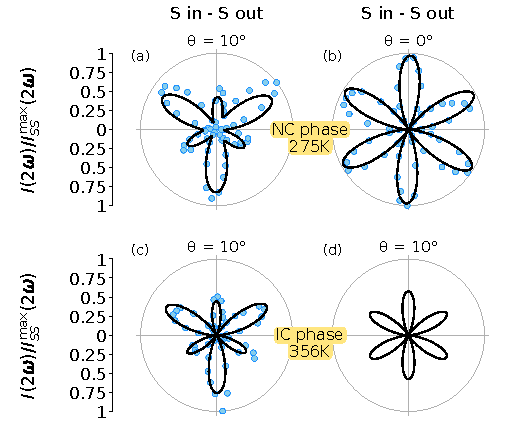
\includegraphics{fig3rev.pdf}
\caption{\label{fig:fig3} Second harmonic intensity as a function of $\phi$ in the S$_\mathrm{in}$-S$_\mathrm{out}$ polarization channel.
Temperatures, phases and incident angles ($\theta$) are indicated on the figure.
Also shown are fitting curves using the point group assignments
(a) $C_3$ surface and $S_6$ bulk,
(b) $C_3$ surface and $S_6$ bulk,
(c) $C_{3v}$ surface and $S_6$ bulk.
(d) Best fit to data in (c) using $C_{3v}$ surface and $D_{3d}$ bulk.
Data in all plots was normalized to one for clariy.
Other polarization channels are depicted in the supplement\cite{supplementary_materials}.
}
\end{figure}

However, symmetry considerations\cite{supplementary_materials} show that $B_0$ is zero in the presence of mirror symmetry.
If bulk mirror symmetry were fully restored in the IC phase, we would therefore expect the signal to be six-fold symmetric.
Fig.~\ref{fig:fig3}(c) shows that the RA-SHG instead remains three-fold symmetric in this phase, suggesting that the bulk breaks mirror symmetry.
On the other hand, the highest-symmetry surface point group consistent with Figs.~\ref{fig:fig1}(a) and \ref{fig:fig3}(c) is $C_{3v}$, which retains mirror symmetry.
With RA-SHG, it is not possible to deduce the full crystal structure, but we speculate that this discrepancy between surface and bulk symmetries might be attributable to the particular stacking arrangement associated with the CDW above $T_{\mathrm{IC-NC}}$\cite{supplementary_materials}.
This would explain why the surface component, which is measuring the local structure at the surface of the sample~\cite{bloembergen_optical_1968}, is consistent with the existence of mirror symmetry, whereas the bulk component, which measures the global structure of many layers, is not.

\section{Conclusion}

In summary, we have demonstrated here that RA-SHG can be used to identify broken mirror symmetry in crystalline materials.
In addition, we have found that RA-SHG can differentiate between structural configurations related by mirror reflection.
By considering the different symmetry constraints on the S$_\mathrm{in}$-S$_\mathrm{out}$ channel, we have also shown that RA-SHG is sensitive to broken mirror symmetry in the bulk of \tastwo, and have found evidence that the IC phase of this material breaks mirror symmetry in the bulk.
Importantly, our analysis is generalizable beyond the specific case of \tastwo, and therefore opens up the possiblity for RA-SHG to detect mirror symmetry-broken phases and their domain structures in other candidate materials.

\section{Acknowledgments}

We would like to thank Adrian Po and Liang Fu for helpful discussions regarding this work.
This work was supported by the Gordon and Betty Moore Foundation’s EPiQS Initiative Grant GBMF4540 to NG (data analysis and manuscript writing) and Grant GBMF3848 to JGC (instrumentation), Shell through the MIT Energy Initiative (experimental setup and material development) and through DARPA DSO under DRINQS program grant number D18AC00014 (sample growth and data taking).
L.Y. acknowledges support by the STC Center for Integrated Quantum Materials, NSF Grant No. DMR-1231319 and by the Tsinghua Education Foundation.
B.G. gratefully acknowledges the German Academic Exchange Service (DAAD) for supporting his research stay with a fellowship.

\section{Supplemental material}

\subsection{Probing broken mirror symmetry with RA-SHG}
\begin{figure*}
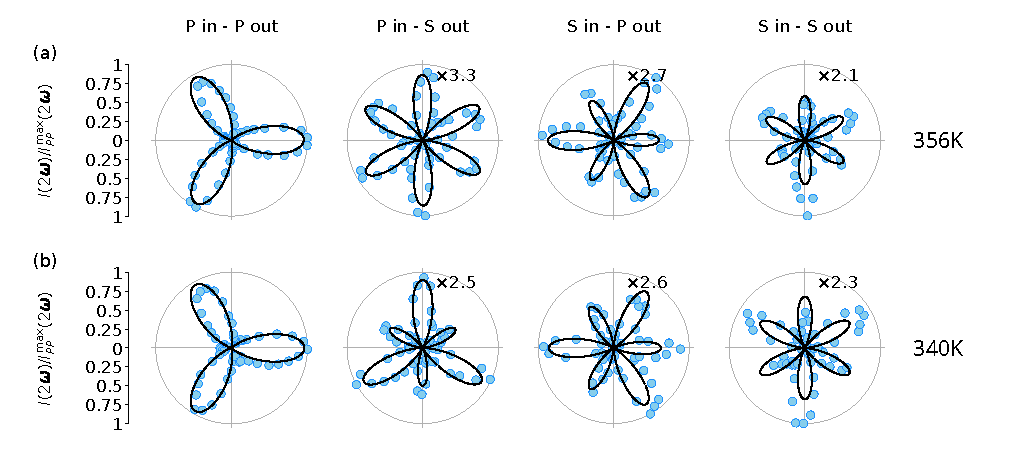
\includegraphics{figS1.pdf}
\caption{\label{fig:figS1}RA-SHG intensity as a function of $\phi$ above (a) and below (b) $T_{IC-NC}=353K$.
Solid lines are are best fits to the data using electric dipole SHG in the surface point groups $C_{3v}$ and $C_3$, respectively.
Data is normalized to the maximum value of the P$_\mathrm{in}$-P$_\mathrm{out}$ signal for each temperature.}
\end{figure*}
\subsubsection{Complete RA-SHG data\label{sec:complete_a}}
In the first section of the main text, we discuss how RA-SHG is sensitive to the breaking of mirror symmetry in \tastwo.
In Figs.~\ref{fig:fig1}(a) and \ref{fig:fig1}(b) of the main text, we display RA-SHG data in two polarization channels: P$_\mathrm{in}$-P$_\mathrm{out}$ and P$_\mathrm{in}$-S$_\mathrm{out}$.
For completeness, the other polarization channels are reproduced in Fig.~\ref{fig:figS1}.
Importantly, the fits in the figure only include a surface electric dipole contribution (see main text).
The inability to fit the S$_\mathrm{in}$-S$_\mathrm{out}$ polarization channel with a pure electric dipole contribution suggested to us that a second contribution was necessary in the form of a bulk electric quadrupole term.
This is discussed in the main text as well as in section \ref{sec:Squadrupole}.

\subsubsection{$\mathscr{I}_{PS}^{(3)}$ as an indicator of broken mirror symmetry\label{sec:Sbmsindicator}}

In the main text, we used the relation given by Eq.~\ref{eq:intensityequation} to show that the breaking of sixfold symmetry in the P$_\mathrm{in}$-S$_\mathrm{out}$ channel is consistent with the lowering of the surface point group from $C_{3v}$ to $C_3$ during the incommensurate (IC) to nearly commensurate (NC) phase transition.
In this section, we show how Eq.~\ref{eq:intensityequation} is derived.

Given any crystallographic point group, it is always possible to compute the form of the susceptibility tensor $\chi^S_{ijk}$.
In $C_3$, the susceptibility tensor is given by~\cite{boyd}
\begin{equation}
\label{eq:Sc3susceptibility}
\chi^S_{ijk} = \begin{pmatrix}
\phantom{-}a & -b & \phantom{-}c\\
-b & -a & -d\\
\phantom{-}c & -d & \phantom{-}0\\
\hline
-b & -a & \phantom{-}d\\
-a & \phantom{-}b & \phantom{-}c\\
\phantom{-}d & \phantom{-}c & \phantom{-}0\\
\hline
\phantom{-}e & \phantom{-}0 & \phantom{-}0\\
\phantom{-}0 & \phantom{-}e & \phantom{-}0\\
\phantom{-}0 & \phantom{-}0 & \phantom{-}f
\end{pmatrix}_{ijk}
\end{equation}
% \begin{equation}
% \label{eq:Sc3susceptibility}
% \chi^S_{ijk} = \begin{pmatrix}
% \chi_{xxx} & -\chi_{yyy} & \chi_{yyz}\\
% -\chi_{yyy} & -\chi_{xxx} & -\chi_{yxz}\\
% \chi_{yyz} & -\chi_{yxz} & 0\\
% \hline
% -\chi_{yyy} & -\chi_{xxx} & \chi_{yxz}\\
% -\chi_{xxx} & \chi_{yyy} & \chi_{yyz}\\
% \chi_{yxz} & \chi_{yyz} & 0\\
% \hline
% \chi_{zyy} & 0 & 0\\
% 0 & \chi_{zyy} & 0\\
% 0 & 0 & \chi_{zzz}
% \end{pmatrix}_{ijk}.
% \end{equation}
for some $a$, $b$, $c$, $d$, $e$, and $f$ which are dependent on the material.
Here, the threefold axis is taken to be along the $z$ direction.
In the point group $C_{3v}$, the susceptibility tensor is constrained by symmetry so as to take a form which is the same as equation \ref{eq:Sc3susceptibility}, but with $b = d = 0$, i.e.

\begin{equation}
\label{eq:Sc3vsusceptibility}
\chi^S_{ijk} = \begin{pmatrix}
\phantom{-}a & \phantom{-}0 & \phantom{-}c\\
\phantom{-}0 & -a & \phantom{-}0\\
\phantom{-}c & \phantom{-}0 & \phantom{-}0\\
\hline
\phantom{-}0 & -a & \phantom{-}0\\
-a & \phantom{-}0 & \phantom{-}c\\
\phantom{-}0 & \phantom{-}c & \phantom{-}0\\
\hline
\phantom{-}e & \phantom{-}0 & \phantom{-}0\\
\phantom{-}0 & \phantom{-}e & \phantom{-}0\\
\phantom{-}0 & \phantom{-}0 & \phantom{-}f
\end{pmatrix}_{ijk}.
\end{equation}
% \begin{equation}
% \label{eq:Sc3vsusceptibility}
% \chi^S_{ijk} = \begin{pmatrix}
% 0 & -\chi_{yyy} & \chi_{yyz}\\
% -\chi_{yyy} & 0 & 0\\
% \chi_{yyz} & 0 & 0\\
% \hline
% -\chi_{yyy} & 0 & 0\\
% 0 & \chi_{yyy} & \chi_{yyz}\\
% 0 & \chi_{yyz} & 0\\
% \hline
% \chi_{zyy} & 0 & 0\\
% 0 & \chi_{zyy} & 0\\
% 0 & 0 & \chi_{zzz}
% \end{pmatrix}_{ijk}.
% \end{equation}
Here, the mirror planes are taken to be the $xz$-plane and those related to it by rotation about the $z$-axis through $\pm \ang{120}$.

To compute the RA-SHG intensity in the P$_\mathrm{in}$-S$_\mathrm{out}$ channel, we consider a frame of reference in which the plane of incidence is held fixed and the sample is rotated about the optical axis.
This reference frame is equivalent to that of the experimental setup (where the sample is fixed and the plane of incidence rotates), but it is easier to visualize and formulate mathematically.
In this frame, the incoming $P$-polarized light at frequency $\omega$ is parallel to the vector $E_i(\omega) = (-\cos{\theta}, 0, \sin{\theta})^T_i$, and the outgoing $S$-polarized light which we wish to compute is parallel to the $y$-axis.
The RA-SHG intensity in this channel is therefore given by
\begin{equation}
\label{eq:Sipsequation}
I_{PS}^{2\omega}(\phi) \propto \left|P_y^{2\omega}(\phi)\right|^2 \propto \left|\bar{\chi}^S_{yjk}(-\phi)E_j(\omega)E_k(\omega)\right|^2,
\end{equation}
where $\bar{\chi}^S_{ijk}(\phi)$ is the susceptibility tensor corresponding to the sample when it has been rotated by an angle $\phi$.
The relative sign in the argument of $\bar{\chi}^S_{ijk}$ is due to the different reference frame used here compared to Fig.~\ref{fig:fig0}(b), where $\phi$ is defined.

With the rotation matrix
\begin{equation}
R(\phi)_{ij} = \begin{pmatrix}
\cos{\phi} & -\sin{\phi} & 0 \\
\sin{\phi} & \cos{\phi} & 0 \\
0 & 0 & 1
\end{pmatrix}_{ij},
\end{equation}
$\bar{\chi}^S_{ijk}(\phi)$ is given by
\begin{equation}
\label{eq:Srotatechi}
\bar{\chi}^S_{ijk}(\phi) = R(\phi)_{il}R(\phi)_{jm}R(\phi)_{kn}\chi^S_{lmn}.
\end{equation}
Substituting Eq.~\ref{eq:Srotatechi} into Eq.~\ref{eq:Sipsequation}, we then have
\begin{equation}
\label{eq:SintensityequationwithR}
I_{PS}^{2\omega}(\phi) \propto \left|R(-\phi)_{yl}R(-\phi)_{jm}R(-\phi)_{kn}\chi^S_{lmn}E_j(\omega)E_k(\omega)\right|^2.
\end{equation}

With Eq.~\ref{eq:Sc3susceptibility} as $\chi^S_{ijk}$, we arrive at Eq.~\ref{eq:intensityequation} in the main text,
\begin{equation}
\label{eq:Sipsequationfinal}
I_\mathrm{PS}(2\omega) \propto (A_0 + A_1\cos{(3\phi)} + A_2\sin{(3\phi)})^2,
\end{equation}
where
% \begin{equation}
% A_0 = -2\chi_{yxz}\sin(\theta)\cos(\theta),
% \end{equation}
% \begin{equation}
% A_1 = \chi_{xxx}\cos^{2}(\theta),
% \end{equation}
% and
% \begin{equation}
% A_2 = \chi_{yyy}\cos^{2}(\theta).
% \end{equation}
\begin{equation}
\label{eq:sA_0equation}
A_0 = 2d\sin(\theta)\cos(\theta),
\end{equation}
\begin{equation}
\label{eq:sA_1equation}
A_1 = -b\cos^{2}(\theta),
\end{equation}
and
\begin{equation}
\label{eq:sA_2equation}
A_2 = a\cos^{2}(\theta).
\end{equation}
Since $b = d = 0$ in $C_{3v}$, these equations show that $A_0$ and $A_1$ are zero in the presence of mirror symmetry, as cited in the main text.
Furthermore, in $C_{3v}$, Eq.~\ref{eq:Sipsequationfinal} reduces to
\begin{equation}
I_\mathrm{PS}(2\omega) \propto A_2^2\sin^{2}(3\phi),
\end{equation}
which posesses sixfold rotational symmetry.

In the main text, we also remark that the breaking of sixfold rotational symmetry across the IC to NC phase transition can be quantified experimentally by performing a spectral (sine) decomposition of the measured intensity ($I_\mathrm{PS}^{2\omega}(\phi)$) and extracting the third Fourier coefficient, which we called $\mathscr{I}_\mathrm{PS}^{(3)}$.
Here, we define $\mathscr{I}_\mathrm{PS}^{(3)}$ explicitly and show that it is present in \tastwo only when mirror symmetry is broken.

The spectral decomposition for any given polarization channel ($\Gamma_\mathrm{in}$-$\Gamma_\mathrm{out}$) is defined formally by writing
\begin{equation}
\label{eq:fourierdecomposition}
I_{\Gamma_\mathrm{in}\Gamma_\mathrm{out}}^{2\omega}(\phi) = \sum_{n=0}^{\infty} \mathscr{I}_{\Gamma_\mathrm{in}\Gamma_\mathrm{out}}^{(n)} \sin{\left[n\phi + \psi_{\Gamma_\mathrm{in}\Gamma_\mathrm{out}}^{(n)}\right]}.
\end{equation}
This equation defines $\mathscr{I}_{\Gamma_\mathrm{in}\Gamma_\mathrm{out}}^{(n)}$ and $\psi_{\Gamma_\mathrm{in}\Gamma_\mathrm{out}}^{(n)}$ as the amplitude and phase of the $n$-fold Fourier component of the corresponding SHG intensity. 

Using Eqs.~\ref{eq:Sc3susceptibility},~\ref{eq:SintensityequationwithR}, and~\ref{eq:fourierdecomposition}, we can then compute $\mathscr{I}^{(3)}_\mathrm{PS}$ and $\psi_{PS}^{(3)}$ in the low temperature phase as 
\begin{equation}
\label{eq:i3PS}
\mathscr{I}_{PS}^{(3)}(\chi^S_{ijk}) \propto 4\sqrt{C_1^2+C_2^2}
\end{equation}
and
\begin{equation}
\psi_{PS}^{(3)}(\chi^S_{ijk}) = \atantwo{\left(C_1,C_2\right)},
\end{equation}
where
\begin{equation}
C_1 = -b\cdot d\sin{\theta}\cos^3{\theta},
\end{equation}
\begin{equation}
C_2 = a\cdot d\sin{\theta}\cos^3{\theta},
\end{equation}
$\theta$ is the angle of incidence, and
\begin{equation}
\atantwo{(y, x)} \equiv \begin{cases}
\arctan{\left(\frac{y}{x}\right)} & x >  0 \\
\arctan{\left(\frac{y}{x}\right)}+\pi & y>0,x <  0\\ 
\arctan{\left(\frac{y}{x}\right)}-\pi & y<0,x <  0\\ 
+\frac{\pi}{2} & y>0, x=0\\
-\frac{\pi}{2} & y<0, x=0\\
\mathrm{undefined}& x = y = 0 \end{cases}.
\end{equation}
By comparing equations \ref{eq:Sc3susceptibility} and \ref{eq:Sc3vsusceptibility}, we find that
\begin{equation}
C_1 = C_2 = 0
\end{equation}
in the high temperature phase, so that $\mathscr{I}_{PS}^{(3)}(\chi^S_{ijk}) = 0$. 
% \begin{equation}
% \label{eq:i3PS}
% \mathscr{I}_{PS}^{(3)}(\chi^S_{ijk}) = 4\sqrt{C_1^2+C_2^2}
% \end{equation}
% and
% \begin{equation}
% \psi_{PS}^{(3)}(\chi^S_{ijk}) = \atantwo{\left(C_1,C_2\right)},
% \end{equation}
% where
% \begin{equation}
% C_1 = -\chi_{yyy}\cdot\chi_{yxz}\sin{\theta}\cos^3{\theta},
% \end{equation}
% \begin{equation}
% C_2 = \chi_{xxx}\cdot\chi_{yxz}\sin{\theta}\cos^3{\theta},
% \end{equation}
% $\theta$ is the angle of incidence, and
% \begin{equation}
% \atantwo{(y, x)} \equiv \begin{cases}
% \arctan{\left(\frac{y}{x}\right)} & x >  0 \\
% \arctan{\left(\frac{y}{x}\right)}+\pi & y>0,x <  0\\ 
% \arctan{\left(\frac{y}{x}\right)}-\pi & y<0,x <  0\\ 
% +\frac{\pi}{2} & y>0, x=0\\
% -\frac{\pi}{2} & y<0, x=0\\
% \mathrm{undefined}& x = y = 0 \end{cases}.
% \end{equation}
% By comparing equations \ref{eq:Sc3susceptibility} and \ref{eq:Sc3vsusceptibility}, we find that
% \begin{equation}
% C_1 = C_2 = 0
% \end{equation}
% in the high temperature phase, so that $\mathscr{I}_{PS}^{(3)}(\chi_{ijk}) = 0$. 

Note that Eq.~\ref{eq:i3PS} highlights an important aspect of our experiment, which is that $\mathscr{I}_{PS}^{(3)}$ requires a nonzero angle of incidence to be observed.
This can be understood by noting that $\mathscr{I}_{PS}^{(3)}$ is nonzero only when the tensor element $\chi^S_{yxz}$ is nonzero.
However, for such a term to be observable in the experiment, there needs to be an out-of-plane component to the incoming electric fields, which in turn requires a nonzero angle of incidence.
Moreover, in a system with three-fold symmetry like \tastwo, the aforementioned tensor element can only be nonzero in a system where mirror symmetry is absent.
To see that this is true, consider the term $P_y(2\omega)=\chi^S_{yxz}E_x(\omega)E_z(\omega)$.
Under an $x \rightarrow -x$ mirror operation, we require that $P_y \rightarrow P_y$, $E_x \rightarrow -E_x$, $E_z \rightarrow E_z$, and $\chi^S_{yxz} \rightarrow \widetilde{\chi}^S_{yxz}$.
However, if this operation is a symmetry of the crystal then we have $\widetilde{\chi}^S_{yxz} = \chi^S_{yxz}$, so that $P_y = -P_y$.
This implies that $\chi^S_{yxz} = 0$.
Therefore both a nonzero angle of incidence and broken mirror symmetry are required for a nonzero $\mathscr{I}_{PS}^{(3)}$ in the geometry of our experiment.

\subsection{Physical importance of the P$_\mathrm{in}$-S$_\mathrm{out}$ channel}

In this section we explain physically why the P$_\mathrm{in}$-S$_\mathrm{out}$ polarization channel is the most sensitive to mirror symmetry breaking in \tastwo.
Consider the experimental geometry depicted in Fig.~\ref{fig:mirror}(a).
A $P$-polarized electric field $\bm{E}_\mathrm{in}$ is incident on a sample with vertical mirror symmetry about the $xz$ plane (indicated by the sides A and B of the sample being the same color). The geometry is such that the plane of incidence makes an angle $\phi$ with the reflection plane.
Let $\bm{P}_\perp(\phi)$ be the $S$-polarized component of the polarization resulting from second harmonic generation by the interaction of the sample with $\bm{E}_\mathrm{in}$.

\begin{figure}
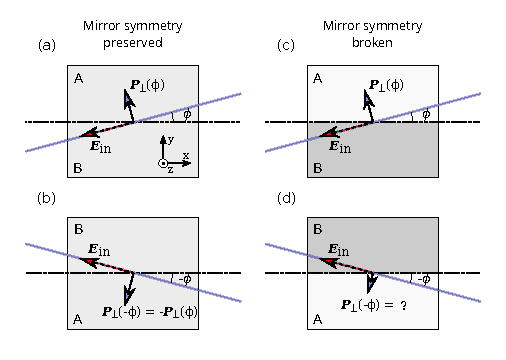
\includegraphics{mirror}
\caption{\label{fig:mirror}(a) Geometry referenced in showing that the P$_\mathrm{in}$-S$_\mathrm{out}$ geometry is sensitive to the breaking of vertical mirror symmetry. $\bm{E}_\mathrm{in}$ is the input electric field and $\bm{P}_\perp$ is the $S$-polarized component of the polarization. The arrow identifying the direction of $\bm{E}_\mathrm{in}$ is dashed to indicate that there is a component in the $z$-direction (out of the page). The solid blue and dotted black lines represent the plane of incidence and the mirror symmetry plane, respectively, which are in the $z$-direction and make an angle $\phi$ with each other. The two halves (A and B) of the sample are the same color to indicate that mirror symmetry is present in this sample. (b) Mirror image of (a), showing that $\bm{P}_\perp$ flips sign (when measured in the frame of the plane of incidence) under mirror reflection. (c) Same geometry as (a) with broken mirror symmetry, represented by the difference in color between sides A and B. (d) Mirror image of (c).}
\end{figure}

Now consider applying the mirror operation both to $\bm{E}_\mathrm{in}$ and to the sample (Fig.~\ref{fig:mirror}(b)).
Then the resulting $S$-polarized component of the polarization (in the frame of the plane of incidence) will be $-\bm{P}_\perp(\phi)$.
However, since the sides A and B in Fig.~\ref{fig:mirror}(b) are the same, by symmetry the problem is equivalent to Fig.~\ref{fig:mirror}(a) but with $\phi$ replaced by $-\phi$.
Thus $\bm{P}_\perp(-\phi) = -\bm{P}_\perp(\phi)$, implying that $\bm{P}_\perp(0) = \bm{P}_\perp(\pi) = 0$.
This along with threefold rotational symmetry is sufficient to prove that the RA-SHG pattern from IC-phase \tastwo in the P$_\mathrm{in}$-S$_\mathrm{out}$ polarization channel is purely sixfold-symmetric.
However, in the case where mirror symmetry is broken (Figs.~\ref{fig:mirror}(c-d)) the above argument no longer holds and the constraint $\bm{P}_\perp(-\phi) = -\bm{P}_\perp(\phi)$ is relaxed.
Therefore in \tastwo, $\mathscr{I}_\mathrm{PS}^{(3)}$ is allowed in the NC phase but not in the IC phase.

\renewcommand{\arraystretch}{1.5}
\begin{table*}[t]
\begin{tabular}{c|c|p{8cm}}
\hline
\hline
% \textbf{Initial group} & \textbf{Final group} & \textbf{Indicator(s)} \\
\textbf{Initial group} & \textbf{Final group} & \multicolumn{1}{>{\centering\arraybackslash}m{100mm}}{\textbf{Indicator(s)}}\\
\hline
$T_{d}$ & $T$ & None \\
$T_{d}$ & $D_{2d}$ & None \\
$T_{d}$ & $C_{3v}$ & None \\
$C_{6v}$ & $C_{3v}$ & $\mathscr{I}_{PP}^{(3)}$, $\mathscr{I}_{PP}^{(6)}$, $\mathscr{I}_{PS}^{(0)}$, $\mathscr{I}_{PS}^{(6)}$, $\mathscr{I}_{SP}^{(3)}$, $\mathscr{I}_{SP}^{(6)}$, $\mathscr{I}_{SS}^{(0)}$, $\mathscr{I}_{SS}^{(6)}$ \\
$C_{6v}$ & $C_{2v}$ & $\mathscr{I}_{PP}^{(2)}$, $\mathscr{I}_{PP}^{(4)}$, $\mathscr{I}_{PS}^{(0)}$, $\mathscr{I}_{PS}^{(4)}$, $\mathscr{I}_{SP}^{(2)}$, $\mathscr{I}_{SP}^{(4)}$ \\
$C_{6v}$ & $C_{6}$ & $\mathscr{I}_{PS}^{(0)}$ \\
$C_{4v}$ & $C_{2v}$ & $\mathscr{I}_{PP}^{(2)}$, $\mathscr{I}_{PP}^{(4)}$, $\mathscr{I}_{PS}^{(0)}$, $\mathscr{I}_{PS}^{(4)}$, $\mathscr{I}_{SP}^{(2)}$, $\mathscr{I}_{SP}^{(4)}$ \\
$C_{4v}$ & $C_{4}$ & $\mathscr{I}_{PS}^{(0)}$ \\
$D_{3h}$ & $C_{3h}$ & $\psi_{PP}^{(6)}$$^*$, $\psi_{PS}^{(6)}$$^*$, $\psi_{SP}^{(6)}$$^*$, $\psi_{SS}^{(6)}$$^*$ \\
$D_{3h}$ & $C_{2v}$ & None \\
$D_{3h}$ & $D_{3}$ & $\mathscr{I}_{PS}^{(3)}$ \\
$C_{3h}$ & $C_{3}$ & $\psi_{PP}^{(1)}$$^*$, $\psi_{PP}^{(2)}$$^*$, $\psi_{PP}^{(3)}$$^*$, $\psi_{PP}^{(4)}$$^*$, $\psi_{PP}^{(5)}$$^*$, $\psi_{PP}^{(6)}$$^*$, $\psi_{PS}^{(1)}$$^*$, $\psi_{PS}^{(2)}$$^*$, $\psi_{PS}^{(3)}$$^*$, $\psi_{PS}^{(4)}$$^*$, $\psi_{PS}^{(5)}$$^*$, $\psi_{PS}^{(6)}$$^*$, $\psi_{SP}^{(1)}$$^*$, $\psi_{SP}^{(2)}$$^*$, $\psi_{SP}^{(3)}$$^*$, $\psi_{SP}^{(4)}$$^*$, $\psi_{SP}^{(5)}$$^*$, $\psi_{SP}^{(6)}$$^*$, $\psi_{SS}^{(2)}$$^*$, $\psi_{SS}^{(4)}$$^*$, $\psi_{SS}^{(6)}$$^*$ \\
$C_{3v}$ & $C_{3}$ & $\psi_{PP}^{(3)}$, $\psi_{PP}^{(6)}$$^*$, $\mathscr{I}_{PS}^{(3)}$, $\psi_{PS}^{(6)}$$^*$, $\psi_{SP}^{(3)}$, $\psi_{SP}^{(6)}$$^*$, $\psi_{SS}^{(6)}$$^*$ \\
$C_{3v}$ & $C_{1h}$ & $\mathscr{I}_{PP}^{(1)}$, $\mathscr{I}_{PP}^{(2)}$, $\mathscr{I}_{PP}^{(4)}$, $\mathscr{I}_{PP}^{(5)}$, $\mathscr{I}_{PS}^{(1)}$, $\mathscr{I}_{PS}^{(2)}$, $\mathscr{I}_{PS}^{(3)}$, $\mathscr{I}_{PS}^{(4)}$, $\mathscr{I}_{PS}^{(5)}$, $\mathscr{I}_{SP}^{(1)}$, $\mathscr{I}_{SP}^{(2)}$, $\mathscr{I}_{SP}^{(4)}$, $\mathscr{I}_{SP}^{(5)}$, $\mathscr{I}_{SS}^{(2)}$, $\mathscr{I}_{SS}^{(4)}$ \\
$D_{2d}$ & $S_{4}$ & $\psi_{PP}^{(4)}$$^*$, $\psi_{PS}^{(4)}$$^*$, $\psi_{SP}^{(4)}$$^*$ \\
$D_{2d}$ & $D_{2}$ & $\mathscr{I}_{PS}^{(2)}$ \\
$C_{2v}$ & $C_{2}$ & $\psi_{PP}^{(2)}$$^*$, $\psi_{PP}^{(4)}$$^*$, $\mathscr{I}_{PS}^{(2)}$, $\psi_{PS}^{(4)}$$^*$, $\psi_{SP}^{(2)}$$^*$, $\psi_{SP}^{(4)}$$^*$ \\
$C_{2v}$ & $C_{1h}$ & $\mathscr{I}_{PP}^{(1)}$, $\mathscr{I}_{PP}^{(3)}$, $\mathscr{I}_{PP}^{(5)}$, $\mathscr{I}_{PP}^{(6)}$, $\mathscr{I}_{PS}^{(1)}$, $\mathscr{I}_{PS}^{(2)}$, $\mathscr{I}_{PS}^{(3)}$, $\mathscr{I}_{PS}^{(5)}$, $\mathscr{I}_{PS}^{(6)}$, $\mathscr{I}_{SP}^{(1)}$, $\mathscr{I}_{SP}^{(3)}$, $\mathscr{I}_{SP}^{(5)}$, $\mathscr{I}_{SP}^{(6)}$, $\mathscr{I}_{SS}^{(0)}$, $\mathscr{I}_{SS}^{(2)}$, $\mathscr{I}_{SS}^{(4)}$, $\mathscr{I}_{SS}^{(6)}$ \\
\hline\multicolumn{3}{l}{$^*$\footnotesize{ Measured from $\pi/2$}}\\
\end{tabular}
\caption{Indicators of broken mirror symmetry in mirror-symmetry-breaking transitions between noncentrosymmetric point groups. Values in the rightmost column (defined in Eq.~\ref{eq:fourierdecomposition}) are zero in the initial group and nonzero in the final group. In all cases, the analysis was done in a geometry such that the sample normal is parallel to the broken mirror plane (i.e. the mirror plane is vertical).}
\label{tab:indicators}
\end{table*}

In contrast to the $S$-polarized output ($\bm{P}_\perp(\phi)$), the $P$-polarized output ($\bm{P}_\parallel(\phi)$) does not change sign (as defined in the frame of the plane of incidence) under mirror reflection.
Therefore the constraint for $P$-polarized output is that $\bm{P}_\parallel(\phi) = \bm{P}_\parallel(-\phi)$.
Importantly, this constraint does not forbid fourier components like $\mathscr{I}_\mathrm{PP}^{(3)}$ and $\mathscr{I}_\mathrm{SP}^{(3)}$, even when mirror symmetry is present.

Finally, while the $S_\mathrm{in}$-$S_\mathrm{out}$ channel is subject to the constraint $\bm{P}_\perp(-\phi) = -\bm{P}_\perp(\phi)$, it can also be shown (see section~\ref{sec:sstwofold}) that in the electric dipole regime, $S_\mathrm{in}$-$S_\mathrm{out}$ is twofold-symmetric regardless of the crystallographic point group.
Therefore the $P_\mathrm{in}$-$S_\mathrm{out}$ polarization channel is especially sensitive to the breaking of vertical mirror plane symmetry in the geometry depicted in Fig.~\ref{fig:mirror}.

\subsection{Generalization to other mirror symmetry-breaking transitions}

While the argument above is effective in the case of a $C_{3v}$ to $C_3$ transition (as in \tastwo), the presence or absence of other symmetries in different point groups may call for symmetry arguments which differ from those above.
Therefore, to generalize this work we provide in Table~\ref{tab:indicators} a list of mirror-symmetry-breaking transitions between noncentrosymmetric point groups and identify corresponding terms (like $\mathscr{I}_\mathrm{PS}^{(3)}$ in \tastwo) which adopt nonzero values in the low-symmetry phase.
This table was generated using the same analysis as in section~\ref{sec:Sbmsindicator} for \tastwo. 
Note that while RA-SHG is only nonzero in noncentrosymmetric point groups, it can still be used in centrosymmetric materials because crystal surfaces necessarily break inversion symmetry.

In most of the transitions in Table~\ref{tab:indicators}, $\mathscr{I}_{PS}^{(n)}$ can be used as an indicator of broken mirror symmetry for some $n$.
However, for others the RA-SHG pattern rotates rather than (or in addition to) changing symmetry, which is indicated by a change in the phase $\psi^{(n)}_{\Gamma_\mathrm{in}\Gamma_\mathrm{out}}$ of certain Fourier components.
Additionally, it should be observed that for a minority of the transitions in Table~\ref{tab:indicators}, RA-SHG is not sensitive to the breaking of mirror symmetry (e.g. in the transition from $T_d$ to $T$, two point groups for which the susceptibility tensor is equivalent).

\subsection{Probing the sense of planar chirality with RA-SHG}
\subsubsection{Complete RA-SHG data\label{sec:complete_b}}
As in section \ref{sec:complete_a}, for completeness we reproduce in Fig.~\ref{fig:figS2} the RA-SHG data in the $\alpha$ and $\beta$ charge density wave (CDW) configurations, including the two polarization channels which were truncated from Fig.~\ref{fig:fig2} in the main text.
The poor fit in the S$_\mathrm{in}$-S$_\mathrm{out}$ polarization channel again indicated to us that there was an additional bulk quadrupole contribution to the signal.

\subsubsection{Electron diffraction confirming the sample is single domain}
To confirm that \tastwo is single-domain in the NC phase, we performed electron diffraction on a sample from the same batch as the one used for the RA-SHG measurements.
The absence of CDW sister peaks in Fig.~\ref{fig:diffraction} demonstrates that the sample is single-domain, in agreement with previous reports~\cite{zong_ultrafast_2018, wilson_charge-density_1975, bovet_pseudogapped_2004, shiba_phenomenological_1986}.
The thickness of the sample measured by electron diffraction was $\sim\qty{80}{nm}$, which is approximately equal to the penetration depth of \tastwo at $\qty{800}{nm}$~\cite{mann_probing_2016}.
We note that recent studies have demonstrated that it is possible to inject mirror domains into an otherwise uniform sample of \tastwo using intense pulses of light~\cite{zong_ultrafast_2018}.
To control for this effect, we used an incident fluence of \qty{1.4}{mJ/cm^2} which is well below the threshold fluence \qty{5}{mJ/cm^2} reported in Ref.~\onlinecite{zong_ultrafast_2018}.

\begin{figure*}
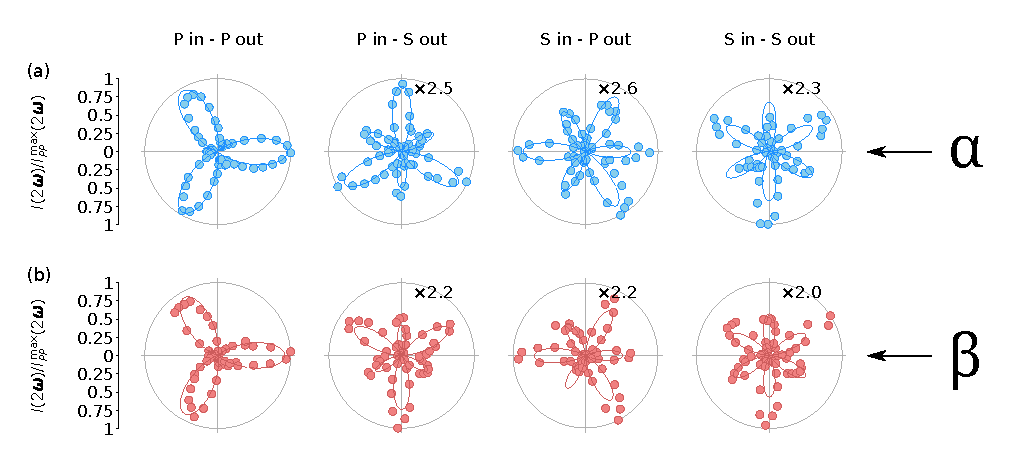
\includegraphics{figS2.pdf}
\caption{\label{fig:figS2}Second harmonic intensity as a function of $\phi$ from two samples of \tastwo in the NC phase ($T=340K$).
The labels $\alpha$ and $\beta$ refer to the two degenerate mirror-image configurations which can exist in the NC phase.
The solid line in (a) is a fit to the data using the surface point group $C_3$.
The fit in (b) was generated by performing a mirror operation (see section \ref{sec:mirrorflip}) to the numerical susceptibility tensor obtained from (a).
Data is normalized to the maximum value in the P$_\mathrm{in}$-P$_\mathrm{out}$ polarization channel for each sample.}
\end{figure*}


\subsubsection{Fitting RA-SHG data in the $\alpha$ and $\beta$ configurations}
\label{sec:mirrorflip}
To fit the data in Fig.~\ref{fig:fig2} of the main text, we performed the following procedure.
First, we used the six independent elements in the $C_{3}$ susceptibility tensor given by equation \ref{eq:Sc3susceptibility} as fitting parameters to fit the data on the $\alpha$ sample (Fig.~\ref{fig:figS2}(a)) to 
\begin{equation}
|P_i(\phi)|^2 \propto |R(-\phi)_{il}R(-\phi)_{jm}R(-\phi)_{kn}\chi_{lmn}^SE_j(\omega)E_k(\omega)|^2.
\end{equation}
The fit was constrained in such a way as to forbid large changes in the susceptibility elements that exist in both phases (i.e. $a$, $c$, $e$, and $f$).
This gave us a set of six numbers $\{\chi_{ijk}^\alpha\}$, from which we can form the tensor $\chi_{ijk}^\alpha$.
The cleaving operation can be represented by the operator $\mathcal{C} = A\Gamma(\gamma)R_x$, where $R_x$ is the operator which rotates the sample \ang{180} about the $x$-axis,
\begin{equation}
\label{eq:chiralityswitcher}
R_x = \begin{pmatrix}
1 & 0 & 0 \\
0 & -1 & 0 \\
0 & 0 & -1 \\
\end{pmatrix},
\end{equation}
$\Gamma(\gamma)$ is the operator which rotates the sample about the $z$-axis by an arbitrary angle $\gamma$,
\begin{equation}
\Gamma(\gamma) = \begin{pmatrix}
\cos{\gamma} & -\sin{\gamma} & 0 \\
\sin{\gamma} & \cos{\gamma} & 0 \\
0 & 0 & 1
\end{pmatrix},
\end{equation}
and $A$ is a positive overall constant which represents minor, day-to-day fluctuations in experimental conditions.
If we were able to cleave the sample exactly along the high-symmetry axis, then $\gamma$ would be \ang{0} and $\Gamma(\gamma)$ would be identity.
Also note that the fact that the determinant of $\mathcal{C}$ in the $(x, y)$ subspace is $-1$ is equivalent to the statement that $\mathcal{C}$ switches the planar chirality of the sample.

To simulate the effect of cleaving the sample, we therefore applied $\mathcal{C}$ to $\chi_{ijk}^\alpha$ to form $\chi_{ijk}^\beta(\{\chi_{ijk}^\alpha\}, \gamma, A)$.
Formally, this amounts to computing
\begin{equation}
\label{eq:SapplyingC}
\chi_{ijk}^\beta(\{\chi_{ijk}^\alpha\}, \gamma, A) = \mathcal{C}_{il}(\gamma, A)\mathcal{C}_{jm}(\gamma, A)\mathcal{C}_{kn}(\gamma, A)\chi_{lmn}^\alpha.
\end{equation}

Now, $\chi_{ijk}^\beta(\{\chi_{ijk}^\alpha\}, \gamma, A)$ is a function of only two free parameters ($\gamma$ and $A$).
We find that with the proper choice of $\gamma$ and $A$, the signal computed with $\chi_{ijk}^\beta$ collapses onto the data in Fig.~\ref{fig:figS2}(b).

By applying $R_x$ to the tensor given in Eq.~\ref{eq:Sc3susceptibility}, one can see that the effect of cleaving the sample is to flip the sign of $b$ and $d$.
By examing Eqs.~\ref{eq:Sipsequationfinal}-\ref{eq:sA_2equation}, and noting that $A_1\approx 0$ within the resolution of our instrument, we see that this reproduces the change of the orientation of the RA-SHG pattern in the P$_\mathrm{in}$-S$_\mathrm{out}$ channel depicted in Fig.~\ref{fig:fig2} of the main text.

\subsection{Bulk broken mirror symmetry in \tastwo} \label{sec:Squadrupole}

\subsubsection{Complete RA-SHG data at $T=295K$}

As in section~\ref{sec:complete_b}, for completeness we reproduce in Fig.~\ref{fig:295K} the RA-SHG data at $T=295K$ (NC phase) which is used in Fig.~\ref{fig:fig3} to argue that there is a nonzero bulk electric quadrupole component to the measured signal.
Furthermore, we reproduce in Fig.~\ref{fig:356K} the RA-SHG data at $T=356K$ (IC phase) to show that we can fit all four polarization combinations using the surface point group $C_{3v}$ as well as a bulk point group $S_6$, which is the highest-symmetry subgroup of the undistorted point group which breaks mirror symmetry (see below).
The S$_\mathrm{in}$-S$_\mathrm{out}$ channel of Fig.~\ref{fig:356K} is shown in Fig.~\ref{fig:fig3} of the main text.

\subsubsection{Symmetry analysis of RA-SHG data} \label{sec:sstwofold}

In the last section of the main text, we used the relation given by Eq.~\ref{eq:qintensityequation} to argue that the breaking of sixfold symmetry in the S$_\mathrm{in}$-S$_\mathrm{out}$ polarization channel indicates that bulk mirror symmetry is broken in the IC phase of \tastwo.
Here we derive Eq.~\ref{eq:qintensityequation} as we did Eq.~\ref{eq:intensityequation} in section~\ref{sec:Sbmsindicator}.

As mentioned in the main text, the effective polarization for bulk electric quadrupole SHG is given by~\cite{kumar_magnetic_2017, shen}
\begin{equation}
\nabla_j Q_{ij} = 2i\chi_{ijkl}^Qk_j E_k E_l,
\end{equation}
so that the total intensity in the S$_\mathrm{in}$-S$_\mathrm{out}$ channel (including surface electric dipole) is given by
\begin{equation}
\label{eq:SQintensity}
I_{SS}^{2\omega}(\phi) \propto \left|\left(\bar{\chi}^S_{yjk}(-\phi)+2i \bar{\chi}_{ypjk}^Q(-\phi)k_p\right)E_j(\omega)E_k(\omega)\right|^2,
\end{equation}
where
\begin{equation}
\bar{\chi}^S_{ijk}(\phi) = R(\phi)_{il}R(\phi)_{jm}R(\phi)_{kn}\chi^S_{lmn},
\end{equation}
\begin{equation}
\bar{\chi}^Q_{ipjk}(\phi) = R(\phi)_{il}R(\phi)_{pq}R(\phi)_{jm}R(\phi)_{kn}\chi_{lqmn}^Q,
\end{equation}
and $E_i(\omega) = (0, 1, 0)^T_i$.

In the NC phase of \tastwo, the appropriate assignment for the surface and bulk point groups is given by diffraction measurements~\cite{spijkerman_x-ray_1997} to be $C_3$ and $S_6$, respectively.
Therefore for $\chi^S_{ijk}$ we use the tensor defined by Eq.~\ref{eq:Sc3susceptibility}, and for $\chi^Q_{ijkl}$ we use the tensor given in Ref.~\onlinecite{boyd} for the point group $S_6$ (which for the sake of brevity we do not reproduce here).
With these tensors, we then have
\begin{equation}
\label{eq:Sequationwithbs}
I_\mathrm{SS}(2\omega) \propto (B_0+B_1\cos{(3\phi)}+B_2\sin{(3\phi)})^2,
\end{equation}
with
\begin{equation}
B_0 = \chi^Q_{xyxx}\sin{\theta},
\end{equation}
\begin{equation}
B_1 = \chi^S_{yyy} -\chi^Q_{xzxy}\cos{\theta},
\end{equation}
and
\begin{equation}
B_2 = -\chi^S_{xxx}+\chi^Q_{xzyy}\cos{\theta}.
\end{equation}

Importantly, if bulk mirror symmetry were restored in the IC phase we would have $\chi^Q_{xyxx} = \chi^Q_{xzxy} = 0$, and therefore $B_0=0$. 
This can be checked by inspecting the quadrupole susceptibility tensor for the undistorted bulk point group $D_{3d}$ (which preserves vertical mirror symmetry) defined in Ref.~\onlinecite{boyd}.
\begin{figure}
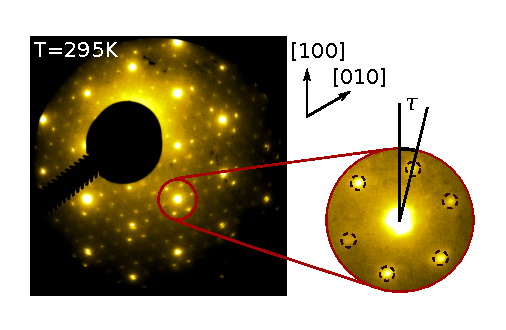
\includegraphics{diffraction.pdf}
\caption{\label{fig:diffraction}Electron diffraction data from a sample of \tastwo in the NC phase of the same batch as the one used in RA-SHG measurements.
Surrounding each Bragg reflection can be seen six CDW peaks, which are rotated about $\tau=\ang{13}$ from the high-symmetry axes.
The sign of the rotation angle $\tau$ indicates whether the CDW configuration is $\alpha$ or $\beta$.
The lack of additional CDW peaks $\ang{-13}$ from the high-symmetry axes indicates that the sample is single-domain.
}
\end{figure}

\begin{figure*}
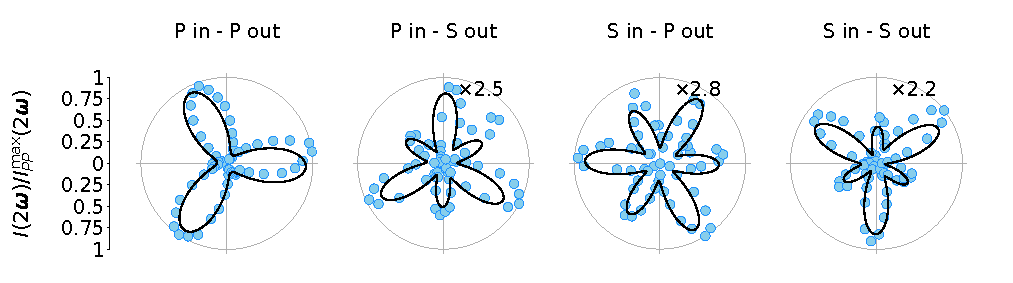
\includegraphics{figS3.pdf}
\caption{\label{fig:295K}RA-SHG intensity as a function of $\phi$ at $T=295K$.
Solid lines are best fits to the data using a surface electric dipole term in the point group $C_3$, as well as a bulk electric quadrupole term in the point group $S_6$.
Data is normalized to the maximum value of the P$_\mathrm{in}$-P$_\mathrm{out}$ signal.}
\end{figure*}

\begin{figure*}
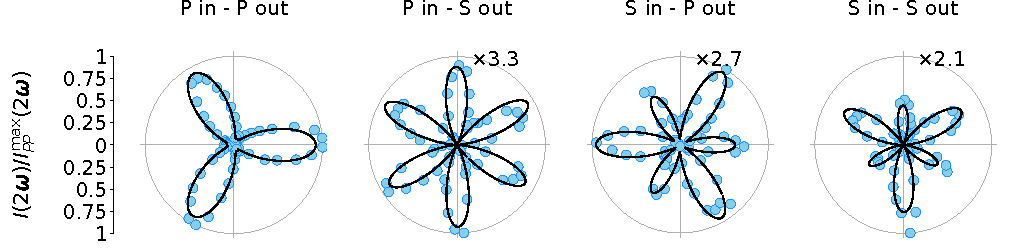
\includegraphics{figS4.pdf}
\caption{\label{fig:356K}RA-SHG intensity as a function of $\phi$ at $T=356K$.
Solid lines are best fits to the data using a surface electric dipole term in the point group $C_{3v}$, as well as a bulk electric quadrupole term in the point group $S_6$.
Data is normalized to the maximum value of the P$_\mathrm{in}$-P$_\mathrm{out}$ signal.}
\end{figure*}
Since $B_0=0$ if the pattern possesses sixfold rotational symmetry (as can be seen by taking $\phi\to\phi+\ang{60}$), we have that the breaking of sixfold rotational symmetry in the RA-SHG pattern (Fig.~\ref{fig:fig3}(c) of the main text) implies $B\neq 0$.
This implies that $\chi^Q_{xyxx} \neq 0$, and therefore mirror symmetry is broken in the bulk.

There are two additional important remarks which can be made about Eq.~\ref{eq:Sequationwithbs}.
For one, it should be noted that the $\theta$ dependence observed in Figs.~\ref{fig:fig3}(a) and~\ref{fig:fig3}(b) is consistent with Eq.~\ref{eq:Sequationwithbs}, since $B_0=0$ for $\theta=0$.
Additionally, we see that in the absence of the quadrupole component (i.e. for purely electric dipole SHG), $B_0 = 0$ and the pattern should have sixfold rotational symmetry.
Since the data in Figs.~\ref{fig:fig3}(a) and~\ref{fig:fig3}(c) clearly break this symmetry, this supports our claim that their is an extra contribution to the RA-SHG beyond the surface electric dipole contribution.

A more intuitive way to understand why the threefold spectral component in Figs.~\ref{fig:fig3}(a) and~\ref{fig:fig3}(c) is not allowed by pure electric dipole SHG is to note that, for purely electric dipole SHG, the rotational anisotropy always has at least twofold symmetry in the S$_\mathrm{in}$-S$_\mathrm{out}$ channel.
To see that this is true, consider the effect of taking $\phi\rightarrow\phi+\pi$ in an $S$-polarized input geometry.
In the frame where the sample is stationary, this simply changes the sign of the input field. 
Since the polarization is proportional to the square of the input field ($P_i(2\omega) = \chi_{ijk}E_j E_k$), then it will be symmetric under $\phi\rightarrow\phi+\pi$, as will be its projection out of the plane of incidence (note, however, that because the component of $\bm{P}(2\omega)$ parallel to the direction of propogation is not visible in the experiment, the same cannot be said for the $P$-polarized output).
Therefore, if the measured RA-SHG in the S$_\mathrm{in}$-S$_\mathrm{out}$ channel lacks twofold symmetry, then there is a contribution to the rotational anisotropy which exists beyond the electric dipole.

For the sake of completeness, we also note here two alternative explanations for the breaking of sixfold rotational symmetry depicted in Fig.~\ref{fig:fig3}(c) which do not appeal to an additional quadrupole contribution.
Firstly, it is possible that the surface of the sample was rough or nonuniform in such a way as to modulate the observed SHG intensity as a function of $\phi$.
In principle, this could result in a nonzero $B_0$.
To account for this artifact, we measured SHG on \tastwo in multiple locations and on multiple different samples, and found that the results in this work were consistent across all measurements.
Furthermore, with SHG measurements there is always the possibility of an additional contribution arising from the presence of adsorbates on the sample surface\cite{berkovic_interference_1988}.
While such a contribution may be present in our experiment, we note that this too is an unlikely explanation for the nonzero $B_0$ because of the wavevector dependence of Figs.~\ref{fig:fig3}(a) and (b).
This is because the dominant contribution from adsorbates is generally of the electric dipole type and therefore should not depend on $\bm{k}$ in S$_\mathrm{in}$-S$_\mathrm{out}$.

\subsection{Methods}

RA-SHG data was taken with the \qty{800}{\nm} pulsed output of a regeneratively amplified Ti:Sapphire laser operating at 5kHz.
The beam was scattered by a transmissive phase grating into multiple diffraction orders, and the +1-order component was steered through a polarizer and focused onto the sample with a fluence of \qty{1.4}{mJ/cm^2} and a spot diameter of $\sim$150$\mu$m at a \ang{10} angle with respect to the $(001)$ sample normal.
This experimental geometry is similar to that described in Refs.~\onlinecite{harter_high-speed_2015} and \onlinecite{torchinsky_low_2014}.
The reflected light at \qty{400}{\nm} was directed through an analyzer and into a photomultiplier tube, where the intensity was measured with a lock-in amplifier synchronized to the 5kHz pulsed output of the laser with a \qty{1}{\ms} time constant.
We rotated the phase grating at $\sim$5Hz and recorded the signal as a function of time with an oscilloscope triggered on an optical rotary encoder marking \ang{360} rotations.
Each polarization combination required averaging 5000 rotations.
Using the aforementioned encoder, we expressed the corresponding time trace in terms of the azimuthal angle $\phi$ (Fig.~\ref{fig:fig0}(b)) to obtain the full rotational anisotropy.

The thickness of the samples used in the RA-SHG experiments was $\sim\qty{50}{\mu m}$.

\chapter{Light-induced reorientation transition in the antiferromagnetic semiconductor \ce{CaMn2Bi2}}\label{ch:cmb}
\section{Preface}

This chapter is based on a manuscript intended for standalone publication and modified to fit the format of this thesis.
It was coauthored by myself and Baiqing Lv (as co-first authors), along with Karna Morey, Zongqi Shen, Changmin Lee, Elizabeth Donoway, Alex Liebman-Pel\'{a}ez, Anshul Kogar, Takashi Kurumaji, Martin Rodriguez-Vega, Rodrigo Humberto Aguilera del Toro, Mikel Arruabarrena, Batyr Ilyas, Tianchuang Luo, Peter M\"{u}ller, Aritz Leonardo, Andres Ayuela, Gregory A. Fiete, Joseph G. Checkelsky, Joseph Orenstein, and Nuh Gedik.
A detailed description of each author's contributions may be found in \cref{cmb-sec:authorcontributions}.

\section{Abstract}

Due to the lack of a net magnetic moment, antiferromagnets possess a unique robustness to external magnetic fields and are thus predicted to play an important role in future magnetic technologies.
However, this robustness also makes them quite difficult to control, and the development of novel methods to manipulate these systems with external stimuli is a fundamental goal of antiferromagnetic spintronics.
In this work, we report evidence for a metastable reorientation of the order parameter in an antiferromagnetic semiconductor triggered by an ultrafast quench of the equilibrium order via photoexcitation above the band gap.
The metastable state forms less than \qty{10}{ps} after the excitation pulse, and persists for longer than \qty{150}{ps} before decaying to the ground state via thermal fluctuations.
Importantly, this transition cannot be induced thermodynamically, and requires the system to be driven out of equilibrium.
Broadly speaking, this phenomenology is ultimately the result of large magnetoelastic coupling in combination with a relatively low symmetry of the magnetic ground state.
Since neither of these properties are particularly uncommon in magnetic materials, the observations presented here imply a generic path toward novel device technology enabled by ultrafast dynamics in antiferromagnets.

\section{Introduction}

When the Hamiltonian of a system contains multiple interaction strengths of comparable magnitude, the corresponding free energy is often host to a diverse collection of metastable states just barely separated in energy from the true ground state.
This phenomenology results in an extreme sensitivity to external stimuli\citep{zhang_dynamics_2014,basov_electrodynamics_2011,dagotto_complexity_2005}, which can be exploited in an ultrafast way using light to drive transitions between these states\citep{basov_towards_2017,kogar_light-induced_2020,mitrano_possible_2016,fausti_light-induced_2011}.

One important application is in magnetic devices, where the electron spins form an ordered state in equilibrium and may thus be used to store information.
\Glspl{afm} have received special attention in this regard, as they possess zero net magnetic moment and are thus robust to stray magnetic fields from adjacent magnetic devices\citep{jungwirth_antiferromagnetic_2016}.
The dominance of exchange rather than anisotropy energies in the dynamics of spins which are antiferromagnetically ordered also leads to order-of-magnitude faster switching timescales compared to their ferromagnetic counterparts\citep{nemec_antiferromagnetic_2018}.

Importantly, the ground state of an \gls{afm} is typically not unique, with the number of degenerate states (corresponding generically to various rotations of the \gls{afm} \gls{op}) being determined by the number of symmetries which are broken at the magnetic ordering temperature.
In the context described above, this degeneracy invites the possibility of an ultrafast antiferromagnetic device which uses light to switch between these different states.
Moreover, if the symmetry of the magnetic phase is sufficiently low (relative to the parent phase), the number of such states can be quite high, and a multi-step magnetic memory might be constructed which operates via ultrafast reorientation transitions of the \gls{afm} \gls{op} between states that are not anti-parallel.

Broadly speaking, one can distinguish two different approaches for achieving such transitions in real materials.
In the first case, one imagines manipulating the \gls{afm} orientation ``coherently'' by, for example, resonantly driving an infrared-active phonon mode to large amplitude, although this usually requires large electric fields (as the relevant light-matter interactions are usually highly nonlinear\citep{afanasiev_ultrafast_2021}) which are difficult to obtain in the frequency range associated with phonons in crystals.
An alternative mechanism---which has been shown to occur abundantly in \gls{sc}\citep{fausti_light-induced_2011} and \gls{cdw}\citep{kogar_light-induced_2020} systems---is to \textit{quench} the equilibrium order by exciting carriers above the band gap, and then exploit the subsequent relaxation dynamics which may, in the right system, show a preference for one state over the other\citep{sun_transient_2020}.
In contrast to the case of resonant phonon driving, this mechanism involves primarily electronic excitations and therefore requires relatively little energy if the photon frequency is above the band gap.
However, despite successful demonstrations of this approach in nonmagnetic systems\citep{fausti_light-induced_2011,kogar_light-induced_2020}, evidence for this mechanism occurring in \glspl{afm} does not currently exist, and whether the phenomenology described here actually occurs in real magnetic materials remains a fundamental open question.

In this work, we report a light-induced phase transition between nearly degenerate \gls{afm} states in the antiferromagnetic semiconductor \cmb \citep{gibson_magnetic_2015} triggered by an ultrafast quench of the equilibrium \gls{op} with a femtosecond light pulse.
Using \gls{trshg}, a pump-probe technique with the unique ability to track both the magnitude and direction of the \gls{afm} order parameter as a function of time, we find that above-gap optical excitation indeed causes the system to switch to a new, metastable orientation of the \gls{afm} \gls{op}.
The transition is fast (occurring less than \qty{10}{ps} after photoexcitation), requires low pump fluence (\threshold vs. \previousthreshold\citep{afanasiev_ultrafast_2021}), and cannot be induced thermodynamically.
These findings suggest a new way to manipulate \glspl{afm}, and open the door to novel opto-spintronic device architectures exploiting nonequilibrium phase transitions between different nearly degenerate states. 

\section{Results}

\subsection{Equilibrium}

\begin{figure}
\centering{
\phantomsubfloat{\label{cmb-fig0:a}}
\phantomsubfloat{\label{cmb-fig0:b}}
\phantomsubfloat{\label{cmb-fig0:c}}
\phantomsubfloat{\label{cmb-fig0:d}}
}
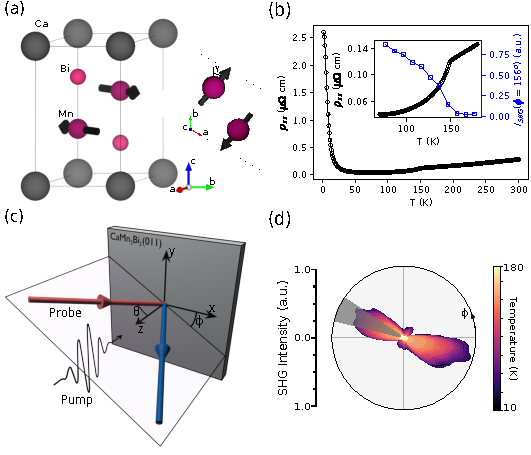
\includegraphics[width=\textwidth]{./gfx/ch6/fig0.pdf}
\captionsetup{singlelinecheck=off}
\caption[Crystal structure of \cmb and temperature dependence of \glsfmtshort{shg}]{
\label{cmb-fig0}
\begin{enumerate*}[label=\caplabel, ref=\capref]
\item Magnetic unit cell of \cmb.
The angle $\gamma$ is such that the \ce{Mn} spin does not lie precisely along any particular crystallographic axis.
\item Resistivity as a function of temperature for a representative sample.
Inset shows an enlarged view of the resistivity near $T_c$ plotted against the SHG intensity integrated across the region indicated in \ref{cmb-fig0:d}.
\item Schematic of the \gls{rashg} setup.
\item Temperature dependence of the \gls{rashg} intensity in the \PP polarization channel from the $(011)$ surface of \cmb.
Other polarization channels are shown in the \supcref{\fulltempdep}.
The shaded area indicates the region integrated to produce the inset of \ref{cmb-fig0:b}.
\end{enumerate*}
}
\end{figure}

Crystallographically, \cmb consists of a puckered-honeycomb tiling of \ce{Mn} atoms with a high-temperature crystallographic point group of \htpg (see \cref{cmb-fig0:a}).
The electronic gap is on the order of \qty{4}{meV} (see \cref{cmb-fig0:b}) and is thought to be due to a delicate combination of correlations and hybridization between relatively localized \ce{Mn} $3d$ states and dispersive \ce{Bi} $6p$ / \ce{Mn} $4s$ hybrid bands\citep{gibson_magnetic_2015, piva_putative_2019, lane_competition_2019}.
N\'{e}el-type antiferromagnetic \gls{lro} with spins lying in the $ab$-plane develops in this material at $T_c=\apx\qty{150}{K}$, accompanied by a kink in the electrical resistivity (\cref{cmb-fig0:b}) and the appearance of a new peak in the powder neutron diffraction\citep{gibson_magnetic_2015}.
Importantly, the powder neutron refinement indicates that the ordered moments are slightly misaligned with the $a$- and $b$-axes of the high-symmetry phase (see \cref{cmb-fig0:a}), so that the low-temperature magnetic point group is $\bar{1}'$; i.e., the only symmetries that are preserved in the low temperature phase are the identity operator and the product of inversion and time-reversal\citep{gibson_magnetic_2015}.
The remarkably low symmetry of this magnetic ground state is likely due to highly frustrated magnetic interactions, as suggested by to the proximity of isostructural \ce{CaMn2Sb2} to a mean-field magnetic tricritical point\citep{mazin_camn2sb2_2013,mcnally_camn2sb2_2015}.
In contrast, the lattice is thought to remain fully symmetric at all temperatures, so that the symmetry-breaking at $T_c$ is solely due to the \gls{afm} order (this is verified with single-crystal \gls{xrd}, see \supcref{cmb-xrd}).

As spin-orbit coupling is expected to be strong in this material, the breaking of inversion symmetry by the magnetic order should result in a strong \gls{shg} signal below $T_c$, despite the fact that the lattice remains centrosymmetric\citep{pan_optical_1989,seyler_spin-orbit-enhanced_2020}.
We probe this \gls{shg} signal using a \gls{rashg} apparatus (\cref{cmb-fig0:c}) which measures the reflected second harmonic intensity as the plane of incidence is rotated about the sample normal\citep{fichera_second_2020, harter_high-speed_2015, torchinsky_low_2014}.
\Cref{cmb-fig0:b,cmb-fig0:d} depict the \gls{shg} signal from the $(011)$ surface of \cmb as a function of temperature across $T_c$, demonstrating that \gls{rashg} is indeed sensitive to the magnetic order in this material.

\begin{figure}
\centering{
\phantomsubfloat{\label{cmb-fig1:a}}
\phantomsubfloat{\label{cmb-fig1:b}}
\phantomsubfloat{\label{cmb-fig1:c}}
\phantomsubfloat{\label{cmb-fig1:d}}
\phantomsubfloat{\label{cmb-fig1:e}}
\phantomsubfloat{\label{cmb-fig1:f}}
\phantomsubfloat{\label{cmb-fig1:g}}
}
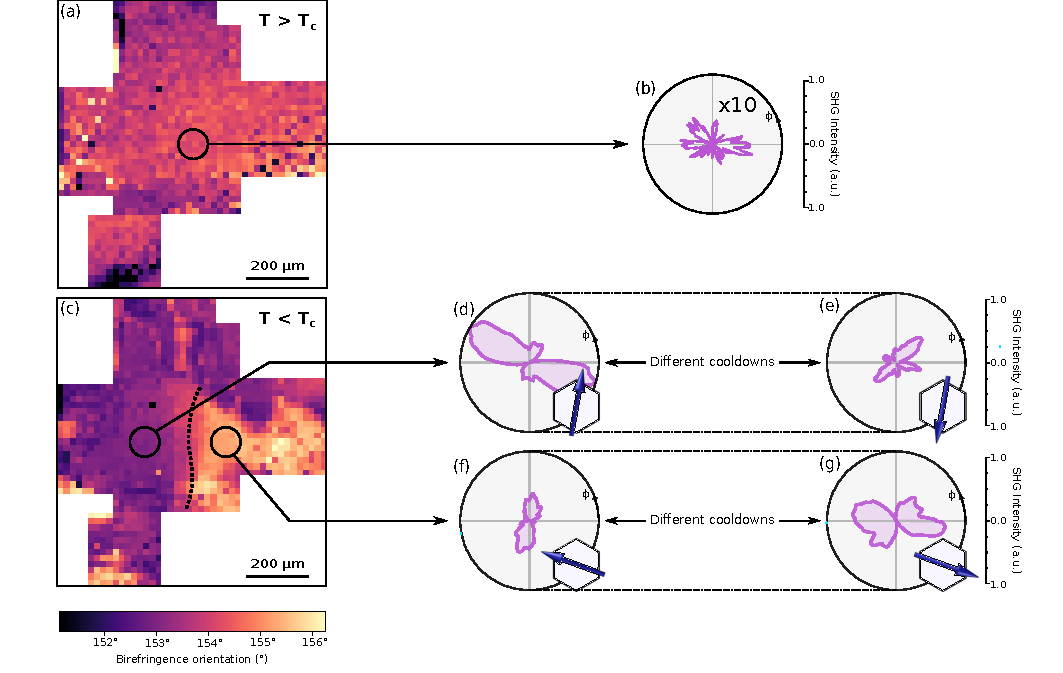
\includegraphics[width=\textwidth]{./gfx/ch6/fig1.pdf}
\captionsetup{singlelinecheck=off}
\caption[Equilibrium domain distribution in \cmb]{
\label{cmb-fig1}
\begin{enumerate*}[label=\caplabel, ref=\capref]
\item Birefringence orientation map for $T=\qty{200}{K}>T_c$.
\item \gls{rashg} intensity in the \PP polarization channel for the region indicated in \ref{cmb-fig1:a} at \qty{157}{K}.
Other polarization channels are shown in the \supcref{cmb-fullequilibrium}.
\item Birefringence orientation map for $T=\qty{152.5}{K}<T_c$.
\item {} \item \gls{rashg} intensity at \qty{8}{K} in the \PP polarization channel for consecutive cooldowns for the region indicated in \ref{cmb-fig1:c}.
The system randomly chooses the \gls{rashg} pattern in \ref{cmb-fig1:d} or \ref{cmb-fig1:e} on each cooldown.
\insets
Other polarization channels are shown in the \supcref{cmb-fullequilibrium}.
\item {} \item \gls{rashg} intensity at \qty{8}{K} in the \PP polarization channel for consecutive cooldowns for the region indicated in \ref{cmb-fig1:c}.
The system randomly chooses the \gls{rashg} pattern in \ref{cmb-fig1:f} or \ref{cmb-fig1:g} on each cooldown.
\insets
Other polarization channels are shown in the \supcref{cmb-fullequilibrium}.
The schematic representations beneath the \gls{rashg} plots are for illustration purposes only and the depicted angles are not quantitatively verified.
\end{enumerate*}
}
\end{figure}

Frequently, \gls{afm} materials may host intricate domain configurations, the details of which greatly impact the relevant magnetic functionalities\citep{reimers_defect-driven_2022, weber_magnetostrictive_2003}.
Because the low-temperature magnetic point group of \cmb breaks multiple symmetries of the high-temperature point group, we indeed expect that the low-temperature magnetic ground state should involve some number of energetically degenerate domains.
In \Cref{cmb-fig1}, we characterize these domains using a combination of \gls{rashg} and a spatially-resolved optical polarimetry technique known as \gls{ptmb}, which is a sensitive technique for measuring small changes in the anisotropic index of refraction (and consequently, the direction of the \gls{afm} \gls{op})\citep{little_three-state_2020, lee_observation_2022}.

\cref{cmb-fig1:a} shows the \gls{ptmb} signal from the $(011)$ surface of \cmb above $T_c$.
No contrast is found within a $\apx\qty{500}{\mu m} \times \qty{500}{\mu m}$ area on the sample, suggesting that the thermally modulated index of refraction is spatially uniform at high temperature.
As the temperature is lowered below $T_c$ (\cref{cmb-fig1:c}), a pronounced contrast appears in the \gls{ptmb} map which indicates the presence of two separate \gls{afm} domains with different \gls{op} directions.

While \gls{ptmb} is nominally sensitive to the direction of the \gls{afm} \gls{op}, it cannot differentiate between \ang{180} domains as it couples only to the linear index of refraction of the material.
Therefore, it is not clear from \gls{ptmb} alone whether the domains in \cref{cmb-fig1:c} are truly homogeneous or may contain a mixture of \ang{180} domains.
In contrast, nonlinear spectroscopies like \gls{shg} can differentiate \ang{180} \gls{afm} domains due to an interference between the \gls{shg} sources (e.g. electric dipole, magnetic dipole, and electric quadrupole) which transform differently under time-reversal symmetry\citep{fiebig_second-harmonic_2005, fiebig_second_1994, fiebig_second_2001, fiebig_domain_1995}.
This effect can be especially pronounced in the presence of magnetostriction\citep{fiebig_second_2001}.
We thus proceed to investigate the presence of \ang{180} domains in this material using \gls{rashg}.

\crefrange{cmb-fig1:d}{cmb-fig1:g} depict the \gls{rashg} results at \qty{8}{K} in the two regions identified in \cref{cmb-fig1:c}.
The same crystal piece was used for both measurements.
As with \gls{ptmb}, we do find that the \gls{shg} domains are large and apparently homogenous (on a scale of hundreds of \si{$\mu$ m}).
Surprisingly, however, in different cooldowns we observe that the \gls{rashg} pattern in the leftmost region of \cref{cmb-fig1:c} randomly takes the form of either \cref{cmb-fig1:d} or \cref{cmb-fig1:e}, and in the rightmost region, it takes the form of either \cref{cmb-fig1:f} or \cref{cmb-fig1:g}.
In contrast, the \gls{ptmb} does not change upon thermal cycling.
Anticipating again that \gls{rashg} should be sensitive to the phase of the \gls{afm} \gls{op} as well as its direction, we interpret \cref{cmb-fig1} as follows: \cref{cmb-fig1:d} and \cref{cmb-fig1:e} correspond to opposite \ang{180} \gls{afm} domains, as do \cref{cmb-fig1:f} and \cref{cmb-fig1:g}; in addition, there is a relative angle between \crefrange{cmb-fig1:d}{cmb-fig1:e} and \crefrange{cmb-fig1:f}{cmb-fig1:g}, as indicated by the \gls{ptmb}.
This interpretation is depicted schematically in the insets to \crefrange{cmb-fig1:d}{cmb-fig1:g}, where the \gls{afm} \gls{op} (defined as the difference in the magnetic moment on the two \ce{Mn} sublattices, see \cref{cmb-fig0:a}) is represented by a blue arrow.
Importantly, within a single location, the two opposite orientations are accessible via thermal cycling; hence they are energetically degenerate.
We have verified that the identification described here is consistent with the \gls{shg} susceptibility tensors\citep{boyd} extracted by fitting the data in \cref{cmb-fig1} (see \supcref{cmb-sec:fitting}).
In addition, the data presented in \cref{cmb-fig1} is not consistent with an alternative interpretation involving the interference of two independent order parameters (see \supcref{cmb-sec:alternativeinterpretation}).

\subsection{Nonequilibrium}
\begin{figure}
\centering{
\phantomsubfloat{\label{cmb-fig2:a}}
\phantomsubfloat{\label{cmb-fig2:b}}
\phantomsubfloat{\label{cmb-fig2:c}}
\phantomsubfloat{\label{cmb-fig2:d}}
}
\includegraphics[width=\textwidth]{./gfx/ch6/fig2.pdf}
\captionsetup{singlelinecheck=off}
\caption[\Glsfmtshort{trshg} of \cmb]{
\label{cmb-fig2}
\begin{enumerate*}[label=\caplabel, ref=\capref]
\item[] \gls{rashg} intensity at \qty{8}{K} in the \PP polarization channel as a function of time for the \gls{afm} \gls{op} identified in \item \cref{cmb-fig1:d}, \item \cref{cmb-fig1:e}, \item \cref{cmb-fig1:f}, and \item \cref{cmb-fig1:g}.
The pump fluence is set to $\apx \qty{600}{\mu J \cdot cm^{-2}}$.
\insets
Other polarization channels are shown in the \supcref{cmb-fullnonequilibrium}.
The schematic representations beneath the \gls{rashg} plots are for illustration purposes only and the depicted angles are not quantitatively verified.
\end{enumerate*}
}
\end{figure}

Having demonstrated that \cmb hosts an elaborate free energy surface with multiple degenerate or nearly degenerate ground states, we now turn to the question of whether light can be used to manipulate or possibly switch between these states. 
To answer this question, we pump each of the \gls{op} directions identified in \cref{cmb-fig1} at \qty{8}{K} with a $\apx \qty{100}{fs}$ normally incident near-infrared light pulse ($\hbar \omega \approx \qty{1}{eV}$) and probe the \gls{afm} \gls{op} with \gls{rashg} using a subsequent probe pulse.
By varying the delay $\Delta t$ between the two pulses, we create a series of snapshots of the \gls{afm} \gls{op} at different times following excitation.
The results are shown in \cref{cmb-fig2}, where the four rows correspond to the four \gls{op} directions identified in \cref{cmb-fig1}, and the horizontal axis is the time delay between the pump and probe pulses.
The first two rows (\crefrange{cmb-fig2:a}{cmb-fig2:b}) correspond to the leftmost domain in \cref{cmb-fig1:c}, for which it is found that, after pumping, the strength of the \gls{rashg} signal is quickly extinguished.
After a delay of around $\apx \num{8}-\qty{10}{ps}$, the \gls{afm} order recovers so that the shape of the \gls{rashg} pattern is similar to before zero delay up to small changes in the relative peak heights.
The \gls{op} magnitude and direction inferred by this data is depicted schematically in the insets to \crefrange{cmb-fig2:a}{cmb-fig2:b}.

The striking observation is in the latter two rows (\crefrange{cmb-fig2:c}{cmb-fig2:d}), which depict the time-resolved \gls{rashg} results in the rightmost domain of \cref{cmb-fig1:c}.
In this domain, the \gls{rashg} signal again quickly decreases, and the shape does not initially change.
However, roughly $\apx \num{6}-\qty{8}{ps}$ after excitation, the \gls{rashg} pattern abruptly changes shape, so that the pattern after $\apx \qty{10}{ps}$ is equivalent to \cref{cmb-fig2:a}.
Together with the findings of \cref{cmb-fig1}, these results suggest that the final state in \crefrange{cmb-fig2:c}{cmb-fig2:d} is one in which the \gls{afm} \gls{op} direction has indeed been reoriented relative to equilibrium.
Remarkably, one must use light to reach this metastable state as it is not present in thermal equilibrium at this spot.

We performed the above measurements out to $\Delta t \gtrsim \qty{150}{ps}$ (see \supcref{cmb-CtoBlong}) and found that the reoriented state persists at least this long before relaxing back to equilibrium in time for the next pair of pulses to arrive (roughly \qty{200}{$\mu$ s} later).
As the pump fluence is decreased (see \supcref{cmb-fluencedep}), the effect of the excitation is diminished until, at low fluences ($\apx \qty{100}{\mu J \cdot cm^{-2}}$), the final state is equivalent to the initial state, and only small changes to the \gls{shg} (associated with dynamics that do not launch the system into the metastable state) are visible near zero delay.
Interestingly, which of the two opposite directions (\cref{cmb-fig1:d} or \cref{cmb-fig1:e}) the magnetic order favors after excitation is consistent from pulse to pulse, but not from one sample to another (see \supcref{cmb-CtoBshort,cmb-CtoBlong}), suggesting that, below the magnetic ordering temperature, interactions between neighboring domains break the degeneracy between these states.
Finally, we note that no aspect of these observations changes with the polarization of the pump pulse (see \supcref{cmb-polarization}).

\section{Discussion}

Taken together, these considerations indeed point to a \textit{bona fide} ultrafast phase transition in \cmb induced by a femtosecond light pulse.
We now seek to understand, at least qualitatively, the microscopic nature of this transition.
Before discussing the time-resolved data of \cref{cmb-fig2}, we must first understand the equilibrium phenomenology implied by \cref{cmb-fig1}.
Group theory (see \supcref{cmb-sec:nonequilibriumtheory}) suggests that there should be twelve energetically degenerate \gls{op} directions, independent of location on the sample.
However, only two directions are observed per measurement location in our experiment.
This observation is explained by recognizing that local strain fields in the material are expected to pole the \gls{lro} (see \supcref{cmb-sec:equilibriumtheory}), so that certain \gls{op} directions are energetically favored relative to others at a given spot\citep{higo_perpendicular_2022,ni_imaging_2021}.
Since these strain fields may vary from one location to another (the details of which depend subtly on the local growth conditions), different locations on the sample would then show different sets of \gls{rashg} patterns, in agreement with the findings of \cref{cmb-fig1}.
This picture also explains the observation that opposite \gls{afm} configurations are energetically degenerate, as strain itself is inherently symmetric under \ang{180} rotations.

\begin{figure}
\centering{
\phantomsubfloat{\label{cmb-fig3:a}}
\phantomsubfloat{\label{cmb-fig3:b}}
\phantomsubfloat{\label{cmb-fig3:c}}
\phantomsubfloat{\label{cmb-fig3:d}}
\phantomsubfloat{\label{cmb-fig3:e}}
}
\includegraphics[width=\textwidth]{./gfx/ch6/fig3.pdf}
\captionsetup{singlelinecheck=off}
\caption[Illustration of our theoretical understanding of \cmb]{
\label{cmb-fig3}
\begin{enumerate*}[label=\caplabel, ref=\capref]
\item[] Illustration of the dynamics following laser excitation as described in the text.
Ultrafast melting of the \gls{afm} order (\ref{cmb-fig3:a}-\ref{cmb-fig3:b}) is followed by the rapid growth of fluctuations (\ref{cmb-fig3:c}-\ref{cmb-fig3:d}), with the final state (\ref{cmb-fig3:e}) determined by the relative growth rate of different orders.
The fluctuation growth step (\ref{cmb-fig3:c}-\ref{cmb-fig3:d}) may occur with or without a background of coherent oscillations (see \supcref{cmb-sec:fluctuations,cmb-sec:nonequilibriumtheory}).
\end{enumerate*}
}
\end{figure}

Turning now to the nonequilibrium phenomenology (\cref{cmb-fig2,cmb-fig3}), we begin by noting that the sudden suppression of the \gls{shg} intensity at early times indicates that the primary effect of the pump pulse is simply to quench the \gls{afm} \gls{op} (\cref{cmb-fig3:a,cmb-fig3:b}).
According to recent theoretical work \citep{sun_transient_2020, dolgirev_self-similar_2020}, the dynamics following such a quench are governed not by the global minimum of the free energy, but rather by the exponential amplification of spatial \gls{op} fluctuations (\cref{cmb-fig3:c,cmb-fig3:d}), which may occur differently for different orders (\supcref{cmb-sec:fluctuations}).
The final state of the transition (\cref{cmb-fig3:e}) is then determined by which state supports the fastest-growing fluctuations.
In the context of light-induced \gls{sc}\citep{fausti_light-induced_2011,cremin_photoenhanced_2019}, for example, the dominant order in equilibrium is a \gls{cdw}, whose fluctuations naturally involve motion of the massive nuclei and are thus much slower than fluctuations of the \gls{sc} \gls{op}\citep{smallwood_tracking_2012,sun_transient_2020}.
Note that, in the general case, the final state is determined not just by the relaxation rates, but also by their start times; that is, if one order is \textit{quenched} faster than another, fluctuations of that order are afforded a longer period to grow and may thus dominate at long times.

In our system, the relatively slow ($\apx \num{8}-\qty{10}{ps}$, see \cref{cmb-fig2}) recovery timescale indicates that the dynamics of the \gls{afm} \gls{op}, like the \gls{cdw} order of \citet{fausti_light-induced_2011}, also likely involve motion of the atomic nuclei (i.e. magnetoelastic coupling).
However, in contrast to the \gls{cdw}-\gls{sc} competition referred to above, the dominant and subdominant orders in our system correspond not to completely different orders, but rather to different orientations of the same order.
One would thus naively expect the corresponding fluctuations to exhibit more or less the same dynamics.
However, as described above, this naive symmetry of the material is in fact broken at all temperatures by the internal strain; thus, it is appropriate to think of the two non-parallel \gls{afm} orientations as truly distinct orders.
Importantly, it is noted in \citet{sun_transient_2020} that small variations in the density of different fluctuations are exponentially amplified as the system relaxes, so that only a modest difference in the relevant dynamics is sufficient to favor the metastable state as the system recovers.
Such asymmetric amplification of non-parallel \gls{afm} orientations thus likely forms the basis for the reorientation transition in \cmb.

Evidence supporting this picture may be found by examining the time dependence of the \gls{shg} signal at short times (\supcref{cmb-quenchtimes}), before the \gls{op} switches to the metastable state.
In particular, on examining the initial decay rates it can be seen that the \gls{shg} signal corresponding to \cref{cmb-fig2:a} reaches \qty{30}{\percent} of its original value just \qty{0.5}{ps} after zero delay; the equivalent drop in \gls{shg} intensity for \cref{cmb-fig2:c} takes $> \qty{0.5}{ps}$ longer.
That is, the quench dynamics associated with the metastable state are roughly twice as fast as those associated with the equilibrium state.
As a result, long-wavelength fluctuations of the subdominant, metastable order experience a longer period of exponential amplification compared to the equilibrium order, which may explain the dominance of the metastable state at long times.
The metastability of the final state is provided by the fact that the long-term relaxation dynamics are presumably dependent on the thermal nucleation and subsequent motion of \gls{afm} domain walls, which can be quite slow\citep{parkin_memory_2015,kim_real-space_2022}.
Finally, we remark that while the quench dynamics described here can explain all features of our data, they also likely occur alongside a background of coherent excitations (e.g. coherent phonons, which are observable in time-resolved reflectivity, see \supcref{cmb-pp}) which can couple to the order parameter via the lattice strain (see \supcref{cmb-sec:nonequilibriumtheory}).
While no evidence of these excitations is apparent in our \gls{shg} data, further studies will be needed to determine the extent to which they might still be important.

\section{Conclusion}

To summarize, we have presented evidence of a magnetic reorientation transition in the antiferromagnetic semiconductor \cmb induced by above-gap optical excitation.
Looking forward, we note two ingredients that seem to be most important for the transition demonstrated in this work: low symmetry, so that there are multiple energetic minima in the magnetic phase, and, presumably, some degree of magnetoelastic coupling, so that the different minima are not precisely degenerate in thermal equilibrium.
Neither of these properties are unique to \cmb, and analogous materials may exist with similar light-induced phenomenology. 
The apparently pronounced coupling between light and magnetic order in this material also invites the fascinating possibility that the magnetic order could be manipulated via additional tuning parameters like strain or current.
This is a key prediction of so-called \pt-symmetric systems, in which inversion and time-reversal symmetries are independently broken but the product of the two is preserved\citep{watanabe_group-theoretical_2018, watanabe_nonlinear_2020, watanabe_symmetry_2018}.
Further investigation of these and related compounds could have far-reaching impacts for future opto-spintronic technology.

\section{Methods}

\subsection{Material growth}

Single crystals of \cmb were grown by a \ce{Bi} flux method following \citet{gibson_magnetic_2015}.
The starting materials were \ce{Ca} ingot, \ce{Mn} powder, and \ce{Bi} powder.
They were loaded into an alumina crucible in the molar ratio of $\ce{Ca}:\ce{Mn}:\ce{Bi} = 1:2:10$, which was sealed in an evacuated quartz tube.
The ampoule was heated to $1000^\circ$\si{C} and kept at this temperature for $11$ hours before being slowly cooled to $400^\circ$\si{C} in $10$ days.
The excess flux was removed by a centrifuge at this temperature.
The single phase nature of the crystals was checked by powder \gls{xrd} and the orientation was checked by a single-crystal x-ray diffractometer.

\subsection{\Glsfmtshort{trshg} measurements}

The \gls{trshg} measurements were performed using a fast-rotating optical grating method which has been described previously\citep{fichera_second_2020, harter_high-speed_2015, torchinsky_low_2014}.
Ultrashort ($\apx \qty{100}{fs}$) probe pulses were sourced from a regeneratively amplified \ce{Ti}:Sapphire laser operating at a repetition rate of \qty{5}{kHz}.
A portion of the \ce{Ti}:Sapphire output was directed to an optical parametric amplifier, producing $\apx \qty{1}{eV}$ pump pulses which were delayed relative to the probe pulses with an optical delay line.
The incident probe fluence was $\apx \qty{250}{\mu J \cdot cm^{-2}}$, with the probe spot diameter being $\apx \qty{100}{\mu m}$ at the sample surface, and the pump pulses (with varying fluence) were focused to a spot roughly $\apx \qty{400}{\mu m}$ in diameter.
The pump was normally incident to the sample surface, but the probe was incident with an angle of $\apx \ang{10}$.
The reflected \gls{shg} signal was collected with a photomultiplier tube, filtered with a lock-in amplifier operating at the repetition rate of the regenerative amplifier, and correlated with the rotation angle of the grating with an optical rotary encoder and homebuilt oscilloscope.
To eliminate potential artifacts due to low-frequency fluctuations in the laser intensity, multiple random sweeps of the delay stage were averaged together for each dataset, and the polarizers were controlled automatically at each delay using custom polarization rotators described in \citet{morey_automated_2024}.

\subsection{\Glsfmtshort{ptmb} measurements}

The polarization-dependent optical birefringence (linear dichroism) measurements were conducted using the experimental setup detailed in \citet{little_three-state_2020}.
A \qty{633}{nm} probe laser beam was focused onto a \qty{5}{$\mu$ m} spot at surface of the sample, while a \qty{780}{nm} pump/heating beam was similarly focused onto the same location.
To improve the signal-to-noise ratio and eliminate polarization artifacts originating from the experimental setup, the sample temperature was modulated at \qty{2}{kHz} by passing the pump beam through an optical chopper.
The linear dichroism signal was subsequently measured using a standard balanced photodetection scheme and a lock-in amplifier.
Position-dependent measurements of optical birefringence were obtained by scanning the sample position with a piezoelectric scanner.
The dependence of the polarization rotation on the probe polarization angle was fit to a sinusoidal function at each spot, and the phase shift parameter extracted from each fit was plotted in \cref{cmb-fig1:a,cmb-fig1:c}.
Note that the birefringence signal involves contributions from both the lattice and the magnetism, so that the angle extracted from this fit should not be identified with the angle of the \gls{afm} \gls{op}.

\subsection{\Glsfmtshort{xrd} measurements}

\Gls{xrd} data (\supcref{cmb-xrd}) were collected at \qty{100}{K} and \qty{180}{K} on a Bruker-AXS X8 Kappa Duo diffractometer with I\textmu S micro-sources, coupled to a Photon 3 CPAD detector using \ce{Mo} K\textalpha~radiation ($\lambda = \qty{0.71073}{\angstrom}$), performing $\phi$-and $\omega$-scans. 
Reconstructed precession images of the $(0kl)$, $(h0l)$ and $(hk0)$ planes were calculated directly from the diffraction images using algorithms included in the APEX3\citep{apex} software.  

\subsection{Data availability}

Data supporting the figures within this paper and other findings of this study are available from the corresponding author upon request.

\section{Acknowledgments}

The authors thank Clifford Allington, Martin Eckstein, Shiang Fang, Feng Hao, David Hsieh, Honglie Ning, Jia Xu, and Guangua Zhang for several helpful discussions.
The authors also acknowledge the MIT SuperCloud and Lincoln Laboratory Supercomputing Center for providing HPC resources that have contributed to the research results reported within this paper.
B.F., B.L., K.M., Z.S., B.I., T.L., and N.G. acknowledge support from the US Department of Energy, BES DMSE (data taking and analysis), and Gordon and Betty Moore Foundation’s EPiQS Initiative grant GBMF9459 (instrumentation).
C.L., E.D., A.L.-P., and J.O. acknowledge support from the Quantum Materials program under the Director, Office of Science, Office of Basic Energy Sciences, Materials Sciences and Engineering Division, of the US Department of Energy, Contract No. DE-AC02-05CH11231.
G.A.F. gratefully acknowledges support from the NSF through the Center for Dynamics and Control of Materials: an NSF MRSEC under DMR-1720595, NSF DMR2114825, and the Alexander von Humboldt Foundation.
R.H.A.d.T., M.A.,A.L., and A.A. acknowledge support from the Spanish Ministry of Science and Innovation through grants PID2019-105488GB-I00, TED2021-132074B-C32 and PID2022-PID2022-139230NB-I00, the European Commission from the MIRACLE (ID 964450), and the Basque Government through Project No. IT-1569-22.

\section{Author contributions}\label{cmb-sec:authorcontributions}
B.F. and B.L. led the project, under the supervision of N.G.
B.F., B.L., K.M., and A.K. designed the \gls{shg} experiments.
B.F., B.L., K.M., Z.S., and A.K. performed the \gls{shg} measurements.
B.F., B.L., K.M., and Z.S. analyzed the \gls{shg} data.
B.F., B.L., and A.K. conceived of the project.
C.L, E.D., A.L.-P., and J.O. performed and analyzed the \gls{ptmb} measurements.
T.K. and J.C. grew the samples and performed the resistivity measurements.
B.I. and T.L. performed the time-resolved reflectivity measurements.
P.M. performed and analyzed the \gls{xrd} measurements.
M.R.V., G.A.F., R.H.A.d.T., M.A., A.L., and A.A. developed the theoretical models and performed the calculations.
B.F. wrote the paper and supplemental material, except for the supplemental theoretical discussion, which was written by M.R.V. with input from R.H.A.d.T.
All authors assisted in revising the manuscript.

\section{Supplementary Material}

\subsection{Supporting theoretical discussion}

\subsubsection{Equilibrium strain-spin coupling}\label{cmb-sec:equilibriumtheory}

To study the coupling between intrinsic strain and magnetic order in \cmb, theoretical calculations were performed using the \gls{paw} implemented in the \gls{vasp}\citep{kresse_efficient_1996, kresse_from_1999}.
For the exchange and correlation potential, we use the Perdew-Burke-Ernzerhof form of the \gls{gga}, which is further corrected with the Couloumb U parameter following the \gls{gga}+U formulation of Dudarev\citep{dudarev_electron-energy-loss_1998}.
We perform a test calculation of the \gls{pdos} using the HSE06 hybrid functional.
Comparing this with the \gls{gga} and \gls{gga}+U calculations, we determine that for an improved system description, it is necessary to include the terms $U(\ce{Mn})=\qty{4}{eV}$ and $U(\ce{Bi})=\qty{3}{eV}$.
All calculations were performed with a well-converged plane-wave cutoff energy of \qty{700}{eV}, a gamma-centered $15\times15\times8$ Monkhorst-Pack $k$-point mesh, and a Fermi smearing of \qty{20}{meV}.
Atomic coordinates were relaxed until forces in all directions were smaller than \qty{0.5}{meV/\angstrom}.
An energy convergence criterion of \qty{1e-7}{eV} is used.
The atomic valence configuration for Ca, Mn and Bi are 3$s^2$3$p^6$4$s^2$4$p^{0.01}$, 4$s^2$3$d^5$ and 6$s^2$6$p^3$, respectively.
The ground state in the trigonal unit cell shows \gls{afm} order between the Mn atoms with an energy difference of about \qty{200}{meV}.

\begin{figure}
\centering
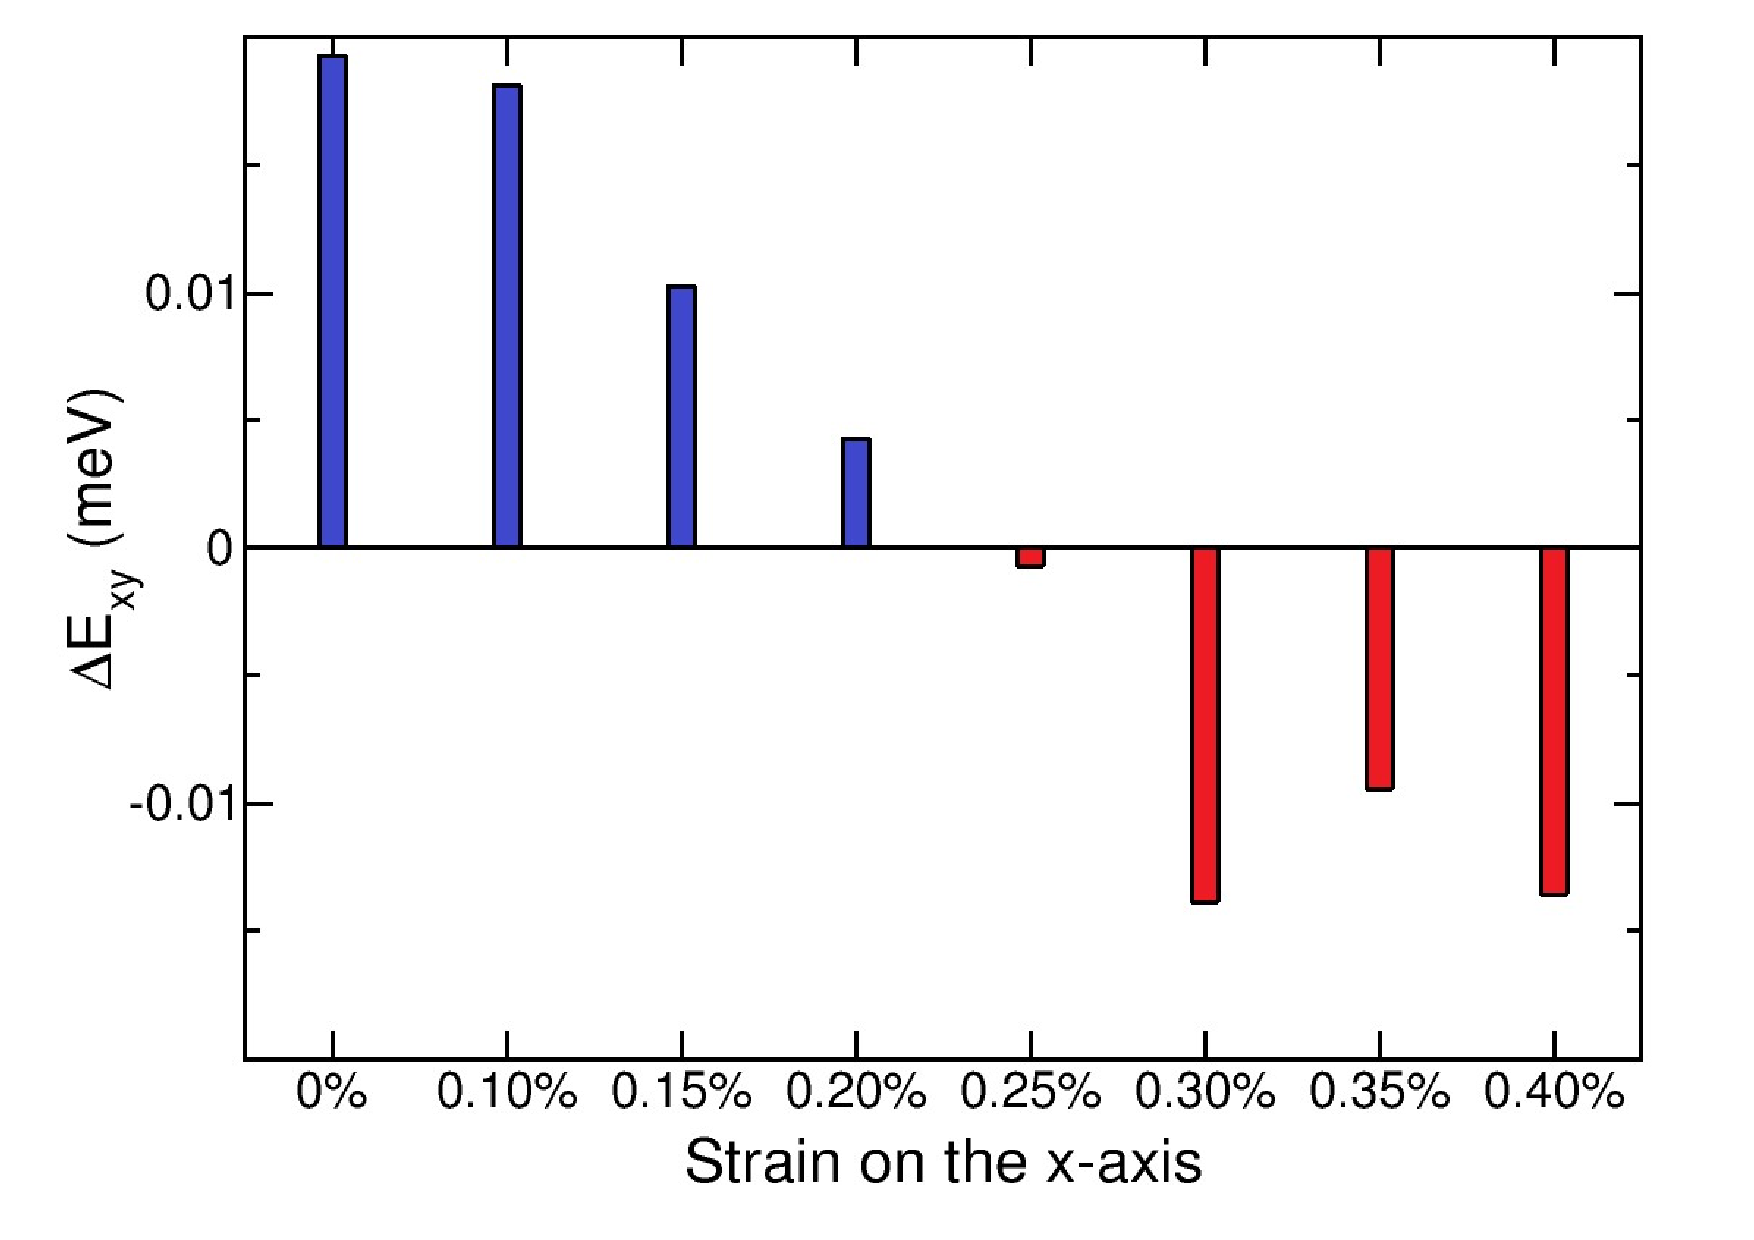
\includegraphics[width=\textwidth]{./gfx/ch6/equilibriumtheory.pdf}
\caption[Energy difference between $x$ and $y$-directions with respect to the easy axis]{
\label{cmb-fig:equilibriumtheory}
Energy difference between $x$ and $y$-directions with respect to the easy axis.
Blue bars indicate the $x$-direction for the \gls{afm} \gls{op} is preferred, and red bars indicate the $y$-direction for the \gls{afm} \gls{op} is preferred.
Note that for strains in experiments, the difference value goes to zero, indicating a change in the in-plane magnetic moment direction.
}
\end{figure}

By including the spin-orbit coupling, we performed additional tests to converge the \gls{mae} with respect to the Brillouin zone sampling.
The spin-orbit coupling energetically favors certain spin orientations in the crystal.
We have determined that the  easy axis is the $x$-axis.
The energy needed to align the spin out-of-plane is \qty{2.4}{meV}, a value that is about a hundred times larger than the \gls{mae} difference with the $y$-axis, which is on the order of \qty{0.02}{meV}.
The \gls{mae} difference with respect  to the $z$-axis remains constant regardless of strain.
The \gls{mae} difference between the $x$ and $y$ directions decreases by applying strain along the $x$-axis, as shown in \cref{cmb-fig:equilibriumtheory}.
With a strain of around $0.25 \%$, the easy spin orientation of the crystal changes to lie along the $y$-axis.

\subsubsection{Laser-induced dynamics of competing magnetic domains: ``incoherent'' scenario}\label{cmb-sec:fluctuations}

In this section, we explore the possibility of interpreting the results of the main text based on the recent quench dynamics theory introduced by Sun and Millis \citep{sun_transient_2020}, and Dolgirev et al. \citep{dolgirev_self-similar_2020}.  

We consider the four observed domains A, B, C, and D as competing AFM orders favored in equilibrium by the local sample anisotropy, regardless of its microscopic origin.
Normally, in the absence of anisotropies, the magnetism in \cmb would be described by model-G \citep{hohenberg1977}.
However, the presence of anisotropies, indicated by the existence of only four domains out of the expected twelve configurations due to symmetry, suggests that total magnetization is not conserved.
Thus, the relaxational behavior of type A studied in detail in \citep{sun_transient_2020,dolgirev_self-similar_2020}, is applicable.
The corresponding relaxational time-dependent-Ginzburg-Landau model is given by $\frac{1}{\gamma_i} \partial_t \psi_i(\mathbf{r}, t)=-\frac{\delta F(t)}{\delta \psi_i(\mathbf{r}, t)}+\eta_i(\mathbf{r}, t),$ where $\psi_i$ corresponds to the staggered magnetization in domain $i=A,B,C,$ and $D.$ $\gamma_i$ and $\eta_i$ are the $i-$th domain relaxation rate and Gaussian white noise source.
The free-energy functional follows the form of Equation (2) in \citep{sun_transient_2020}, with interactions among the domains, $F = \int d^D\mathbf{r} \left(\sum_i f_i+f_c \right)$, $f_i=-\alpha_i \psi_i^2+\left(\xi_{i 0} \nabla \psi_i\right)^2+\psi_i^4$, and $f_c =   \psi^2_C (c_{AC}\psi^2_A+c_{CB}\psi^2_B) + \psi^2_D (c_{AD}\psi^2_A+c_{BD}\psi^2_B)$.
$\xi_{i 0}$ is the bare coherence lengths, and $\alpha_i = \alpha_i(t)$ is a time-dependent dimensionless coefficient influenced by the laser pump excitation's temperature profile.

During the laser pump excitation, characterized by a high temperature and $\alpha_i(t)<0$, and until $\alpha_i(t)=0$, the mean-field order parameters have small values, and the dynamics are governed by order-parameter fluctuations.
Subsequently, the fluctuations grow exponentially, leading to a metastable state determined by the fastest-relaxing domain.
In our experiment, domain A always goes to A, domain B always goes to B, while domain C and D can go to either A or B.
Assuming that the coefficients $\alpha_i$ in equilibrium are equal across the four domains, this observation aligns with the theory prediction if $\gamma_{A/B} > \gamma_{C/D}$ and $\gamma_A \approx \gamma_B$.

\subsubsection{Laser-induced dynamics of competing magnetic domains: ``coherent'' scenario}\label{cmb-sec:nonequilibriumtheory}

\textit{Group theory aspects of the magnetic order}

\cmb belongs to the trigonal symmorphic space group $P\bar 3m1$ (No. $164$) \citep{gibson_magnetic_2015}.
The Wyckoff positions of the atoms are Bi 2d, Mn 2d, and Ca 1a.
The Ca atoms form a triangular lattice on the top and bottom of the Bi and Mn atoms, while Mn and Bi form  buckled hexagonal lattices.
At the $\Gamma$ point, the point group is $\bar{3}m$, which possess twelve symmetry operations: 
%
\begin{itemize}
\item[] $\{ 1 | 0 \}$: $(x,y,z) \rightarrow$ $(x,y,z)$
\item[]  $\{ 3^+_{001} | 0 \}$: $(x,y,z) \rightarrow$ $(-y,x-y,z)$
\item[]  $\{  3^-_{001} | 0 \}$: $(x,y,z) \rightarrow$ $(-x+y,-x,z)$
\item[]  $\{ 2_{110} | 0 \}$: $(x,y,z) \rightarrow$ $(y,x,-z)$
\item[]  $\{ 2_{100} | 0 \}$: $(x,y,z) \rightarrow$ $(x-y,-y,-z)$
\item[]  $\{ 2_{010} | 0 \}$: $(x,y,z) \rightarrow$ $(-x,-x+y,-z)$
\end{itemize}
%
plus their composition with inversion symmetry $\{  -1| 0 \} : (x,y,z) \rightarrow$ $(-x,-y,-z)$.
With this lattice information above the magnetic transition temperature, we proceed with a group theory analysis of the possible magnetic orders with the aid of \small{ISOTROPY} \citep{ISOTROPY}.
In \cmb, the magnetic transition is not accompanied by a lattice deformation, such that the magnetic unit cell coincides with the chemical unit cell.
Therefore, the magnetic order is associated with $\Gamma$ point irreducible representations.
The magnetic subgroups resulting from the onset of all possible $\Gamma$ point irreducible representations are shown in \cref{cmb-tab:irreps_mag}.
The $A_{2g}$ and $A_{1u}$ irreducible representations (irreps) correspond to out-of-plane ferromagnetic and antiferromagnetic order, respectively.
The two-dimensional irreps $E_{g}$ and $E_{u}$ induce in-plane magnetic and \gls{afm} order, respectively.
A general direction of the \gls{op} is associated with the magnetic subgroup $P\bar 1'$, which corresponds to the experimental magnetic space group~\citep{gibson_magnetic_2015}.
Notice that special directions of the \gls{op} lead to magnetic structures with higher symmetry and corresponding magnetic space groups $C2/m'$ or $C2'/m$.

Finally, noting that each of the twelve symmetry operations listed above leads to a different \gls{afm} \gls{op} direction (as the real \gls{op} does not lie along any of the special directions), the free energy surface in equilibrium should have exactly twelve minima in the absence of strain, as referenced in the text.

\begin{table}[h]
\begin{tabular}{|l|l|l|l}
\hline
IR                            & Subgroup & Direction  \\ \hline
$\Gamma_1^+$   ($A_{1g}$)   &  $(164.85) P\bar3m1  $       & P1 (a)    \\ \hline
$\Gamma_2^+$   ($A_{2g}$)   &  $ (164.89) P\bar3m'1 $       & P1 (a)   \\ \hline
\multirow{3}{*}{$\Gamma_3^+$ ($E_{g}$)}  &  $ (12.58) C2/m $    & P1 (a,-1.732a) \\ \cline{2-3} 
                              &   $(12.62) C2'/m'$       &   P2 (a,0.577a)        \\ \cline{2-3} 
                              &   $ (2.4) P\bar1$       &     C1  (a,b)     \\ \hline
$\Gamma_1^-$   ($A_{1u}$)   &  $ (164.88) P\bar3'm'1  $       & P1 (a)   \\ \hline
$\Gamma_2^-$   ($A_{2u}$)   &  $(164.87) P\bar3'm1$       & P1 (a)  \\ \hline 
\multirow{3}{*}{$\Gamma_3^-$ ($E_{u}$)}  &  $(12.60) C2'/m $ & P1 (a,-1.732a)   \\ \cline{2-3}    
                              &   $(12.61) C2/m'$       &   P2  (a,0.577a)     \\ \cline{2-3} 
                              &   $ (2.6) P\bar1'$       &     C1  (a,b)     \\ \hline                         
\end{tabular}
\caption[Subgroups obtained by the onset of magnetic order of a given irreducible representation]{
Subgroups obtained by the onset of magnetic order of a given irreducible representation.
The columns indicate the irreducible representations, the magnetic group, and the \gls{op} direction in the representation space.}
\label{cmb-tab:irreps_mag}
\end{table}

\textit{Free energy model}

Now we construct a free energy model considering magnetic order, strain, and phonon modes.
As discussed in the previous section, the in-plane \gls{afm} groundstate corresponds to the magnetic irrep $\Gamma_3^-$, with general in-plane \gls{op} directions $L_1$,  $L_2$.
The parent cell supports  strain mode distortions with irrep $\Gamma_1^+$ and $\Gamma_3^+$.
We consider a two component $\Gamma_3^+$ mode with components $\epsilon_{xx} = - \epsilon_{yy}$ ($\epsilon_1$) and $\epsilon_{xy}$ ($\epsilon_2$).
Finally, the phonon mode ($Q$) is assumed to be totally symmetric.
The free energy, to fourth order, then takes the form $\mathcal F =\mathcal F_M + \mathcal F_S + \mathcal F_C + \mathcal F_{P}$, with
\begin{align}
    \mathcal F_M  & = (T/T_c - 1) L_1^2 + (T/T_c - 1) L_2^2 + (L_1^2 + L_2^2)^2,\\
    \mathcal F_S  & = \frac{1}{2}(e_1^2 + e_2^2)  + e_1^3 -  e_1 e_2^2 + (e_1^2 + e_2^2)^2,\\
    \mathcal F_P  & = \frac{\omega^2}{2}Q^2 +  Q^3 + Q^4 ,\\
    \mathcal F_C  & = \nonumber (L_1^2-L_2^2) e_1 - L_1 L_2 e_2 + (L_1^2+L_2^2)(e^2_1 + e^2_2) \\ \nonumber &+ L_1 L_2 e_1 e_2 + (L_1^2+L_2^2)(Q+Q^2)+(e^2_1 + e^2_2)(Q+Q^2) \nonumber \\ &+(L_1^2 - L_2^2)e_1 Q -L_1 L_2 e_2 Q+e_1^3Q-e_1 e_2^2 Q.
\end{align}
%
Each of the terms in the model $\mathcal F$ is preceded by a constant whose sign and absolute value cannot be determined within group theory and are sample-dependent.
The magnetic term, $\mathcal F_M$, could include anisotropic terms (due to spin-orbit coupling or single-ion anisotropies, for example), which we omit as the simplest model presented can describe the phenomenology in the experiment. 

We assume that the laser excites the totally-symmetric phonon coherently via a displacive excitation mechanics~\citep{zeiger_theory_1992}.
The laser-phonon coupling term is given by $\mathcal F_l = E_0 \eta(t) Q,$ where $\eta(t) = \kappa \int_0^{\infty} g(t-\tau) e^{-\beta \tau} d \tau,$ and $g(t)$ is the laser pulse shape, and $\beta$ is a parameter associated with rate of electronic relaxation to the groundstate.
The differential equations governing the system can be obtained by taking the variation of the $\mathcal F +\mathcal F_l$ potential with respect to the \gls{afm} \glspl{op}, strain, and phonon.
For the results in the main text, we include phenomenological damping.
The equations of motion are $-\delta (\mathcal F +\mathcal F_l)/\delta \chi_i =  \partial^2_t \chi_i(t)+\gamma_i \partial_t\chi_i(t)$, where  $\chi = \{Q, L_1, L_2\}$ and $\gamma_i$ is the damping coefficient.

\textit{Phonon coupling effect.}

\begin{figure}
\phantomsubfloat{\label{cmb-fig:nonequilibriumtheory1a}}
\phantomsubfloat{\label{cmb-fig:nonequilibriumtheory1b}}
\centering
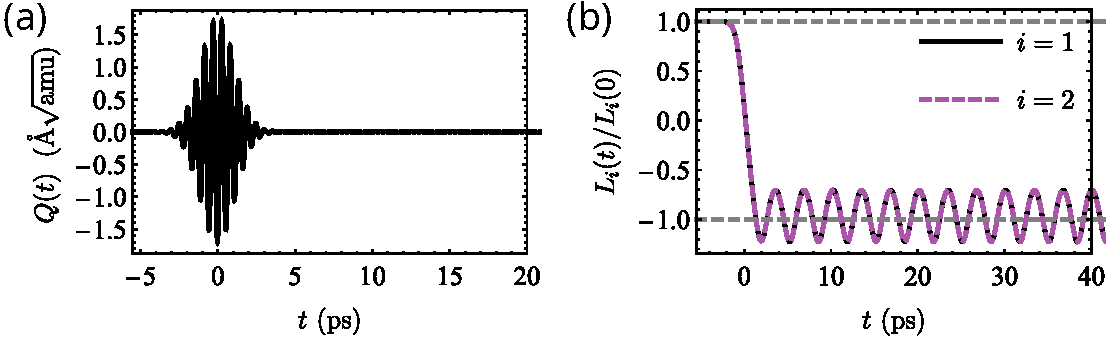
\includegraphics[width=\textwidth]{./gfx/ch6/nonequilibriumtheory1.pdf}
\captionsetup{singlelinecheck=off}
\caption[Phonon mode and \glsfmtshort{afm} \glsfmtlong{op} following photo-excitation with coupling $(L_1^2 + L_2^2)(Q+Q^2)$]{
\label{cmb-fig:nonequilibriumtheory1}
\begin{enumerate*}[label=\caplabel, ref=\capref]
\item Phonon mode and \item \gls{afm} \gls{op} following photo-excitation with coupling $(L_1^2 + L_2^2)(Q+Q^2)$.
\end{enumerate*}
}
\end{figure}

First, we assume that there is no strain in the sample.
The only term linking the \gls{afm} \gls{op} to the time-dependent phonon is $(L_1^2 + L_2^2)(Q+Q^2)$.
We find that this term can lead to flips of $L_1$ and $L_2$ by 180 degrees for long-enough laser pulses. \Cref{cmb-fig:nonequilibriumtheory1a} shows the phonon dynamics following photo-excitation with a $1$eV pulse and duration $\tau =\qty{1.1}{ps}$.
The phonon frequency was assumed to be $\omega/(2\pi) = \qty{3}{THz}$, and the initial temperature is $T=0$.     

\textit{Strain}

\begin{figure}
\centering{
\phantomsubfloat{\label{cmb-fig:nonequilibriumtheory2a}}
\phantomsubfloat{\label{cmb-fig:nonequilibriumtheory2b}}
}
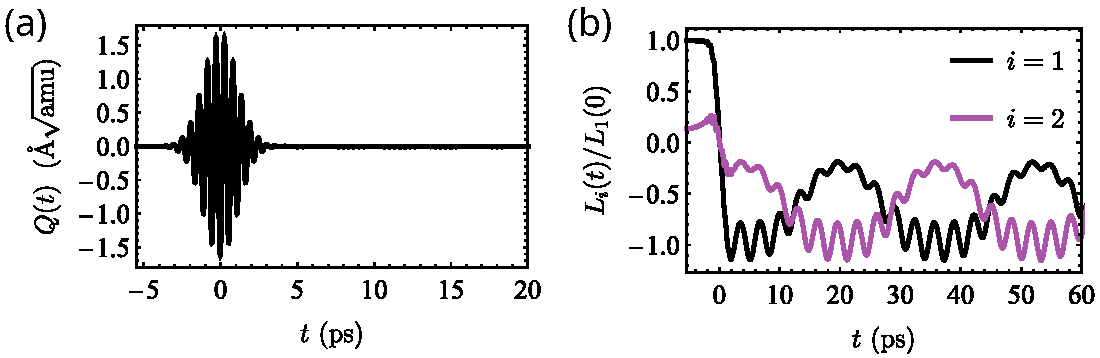
\includegraphics[width=\textwidth]{./gfx/ch6/nonequilibriumtheory2.pdf}
\captionsetup{singlelinecheck=off}
\caption[Phonon mode and \glsfmtshort{afm} \glsfmtlong{op} following photo-excitation with coupling $L_1 L_2 e_2 Q$]{
\label{cmb-fig:nonequilibriumtheory2}
\begin{enumerate*}[label=\caplabel, ref=\capref]
\item Phonon mode and \item \gls{afm} \gls{op} following photo-excitation with coupling $L_1 L_2 e_2 Q$.
\end{enumerate*}
}
\end{figure}

The presence of strain mediates coupling terms between the phonon and the \gls{afm} \gls{op} that can lead to orientations absent in equilibrium.
In particular, the coupling term $L_1 L_2 e_2 Q$ induces a solution where the components $L_1, L_2$ oscillate around a position distinct to the initial configuration and to 180-degree flips.
We consider a pulse with duration $\tau = \qty{1.2}{ps}$, phonon frequency $\omega/(2\pi) = \qty{3}{THz}$, $T=0$, and strains $\epsilon_1 = 0.01$, $\epsilon_1 = 0.05$.
The long-time average of $L_2(t)$ acquires values comparable with $L_1(t)$, as seen in \cref{cmb-fig:nonequilibriumtheory2b}. 

\subsection{Nonviability of secondary order parameter in describing the \gls{rashg} data}\label{cmb-sec:alternativeinterpretation}

Using a combination of \gls{ptmb} and \gls{rashg}, we argue in the main text that, in equilibrium, the magnetism in \cmb that we observe is described by a spatial distribution of four domains $A$, $B$, $C$, and $D$, for which the order parameters satisfy the relations $l_A = -l_B$, $l_C = -l_D$, and $l_C = R(l_A)$, where $R$ is an element of the high-temperature point group \htpg.
In this scenario, the contrast in SHG between e.g. $l_A$ and $l_B$ comes from the fact that there can be two contributions to the \gls{rashg} signal which interfere with each other and transform differently as $l_A \rightarrow l_B$.
That is, we can write
\begin{equation}\label{cmb-eq:eq1}
I_\mathrm{SHG} \propto |e^\mathrm{out}_i \chi_{ijk} e^\mathrm{in}_j e^\mathrm{in}_k|^2,
\end{equation}
where
\begin{equation}\label{cmb-eq:eq2}
\begin{aligned}
\chi_{ijk} &\equiv &&\chione_{ijk} + \chitwo_{ijk}, \\
\end{aligned}
\end{equation}
\begin{equation}
\label{cmb-eq:trrelations}
\begin{aligned}
T (\chione_{ijk}) &= &-&\chione_{ijk}, \\
T (\chitwo_{ijk}) &= &&\chitwo_{ijk},
\end{aligned}
\end{equation}
$T$ is the time-reversal operator which takes $l_A \rightarrow -l_A = l_B$, and $e^\mathrm{in}$ and $e^\mathrm{out}$ are unit vectors in the direction of the polarization of the incoming and outgoing electric fields, respectively.

An important question thus arises: what is the origin of the two sources $\chione$ and $\chitwo$?
The simplest explanation is that both contributions are due to the \gls{afm} \gls{op}; the relations in \cref{cmb-eq:trrelations} are then permitted below $T_c$, where time-reversal symmetry is broken and so $\chi_{ijk}$ can, in general, have parts which transform as both even and odd under time-reversal.
However, an alternative interpretation is that there are in fact two \glspl{op} $l$ and $g$, with $g$ being e.g. some structural \gls{op}, so that, e.g.
\begin{equation}
\label{cmb-eq:proptolg}
\begin{aligned}
\chi^C &\propto l + g, \text{and} \\
\chi^D &\propto l + Rg,
\end{aligned}
\end{equation}
for some $R \in \htpgmathmode$.

In this interpretation, alternative descriptions of the time-resolved results, involving e.g. a melting of $g$ while the $l$ stays fixed, may explain \cref{cmb-fig2}, but not imply a reorientation of $l$ as we claim in the main text.
However, we argue that such an interpretation is not a viable description of our results, both in and out of equilibrium.
% The reasoning can be seen by considering the effect of \cref{cmb-eq:proptolg} on the \gls{rashg} patterns corresponding to domains $C$ and $D$ (see \cref{cmb-fig1} in the main text).
This can be understood by considering the fact that the \gls{rashg} pattern in \cref{cmb-fig1:f} has nodes at $\phi=0$ and $\phi=\pi$ for all temperatures below $T_c$ (see \cref{cmb-ctempdep}).
In the case $Rg = -g$, this suggests that, if there are indeed two independent order parameters contributing to the \gls{rashg} pattern, their amplitudes must exactly cancel for all $T < T_c$.
This is unlikely as the two independent order parameters should in general depend differently on temperature.
Moreover, the case $Rg \neq -g$ is difficult to reconcile in light of the result that the \gls{ptmb} signal is invariant under thermal cycling.
In nonequilibrium, any scenario involving the melting of one \gls{op} while the other stays fixed must also be reconciled with the observation that the nodes in \cref{cmb-fig2:c} in the initial state (before $t=0$) become peaks in the final state.

Furthermore, the above interpretation must also explain how the final state of the transition seems to differ from sample to sample (as explained in the main text; see \cref{cmb-CtoBshort,cmb-CtoBlong}), as well as how the \gls{rashg} is poled in equilibrium to only two of many different degenerate states.
Both of these facts fall out naturally from the assignment presented in the main text.

Together with the lack of a change in the \gls{xrd} across $T_c$ (see \cref{cmb-xrd}), the above considerations suggest that the scenario presented in the main text, which neatly describes the data both in and out of equilibrium, is the most likely.
Future studies will be required to completely truly rule out all alternative scenarios.

\subsection{Fits to susceptibility tensors}\label{cmb-sec:fitting}

In the text, it was remarked that the \gls{op} assignment depicted in \crefrange{cmb-fig1}{cmb-fig2} was consistent with the \gls{shg} susceptibility tensors extracted by fitting the \gls{rashg} patterns.
In this section, we state how this fitting was performed.

Before that discussion, however, we must mention one important point about the predictive power of these fits.
Since the low-temperature point group of \cmb is $\bar{1}'$, the relevant susceptibility tensors are entirely unconstrained and the cost function to be minimized may involve upward of 36 free parameters.
Thus, in principle, many combinations of parameters may fit the data appropriately, thereby limiting the extent to which the \gls{shg} fits can be used to draw conclusions about the underlying state.
One must look to other arguments, e.g. involving \gls{ptmb}, to draw useful conclusions about the data, as was done in the text.
However, once a conclusion has been made, it can at least be checked that a set of fitting parameters \textit{does} exist that is consistent with the conclusion and with the data.
This is the goal of this section.

The \gls{op} assignment discussed in the text involves two parts.
In the first part, the equilibrium SHG in the four domains of \cref{cmb-fig1} is assigned to four different \gls{op} directions, in which the \gls{shg} on consecutive cooldowns on a single spot is due to \ang{180} \gls{afm} configurations, and adjacent spots have a relative angle between them.
As argued in the text, since the \ang{180} domains have different \gls{rashg} patterns, there are most likely two contributions to the \gls{shg} adding coherently to give an interference term, as observed in other magnetic systems\citep{fiebig_second_1994, fiebig_second_2001, fiebig_second-harmonic_2005}.
Designating the four configurations as $A$, $B$, $C$, and $D$ (for \cref{cmb-fig1:d}, \cref{cmb-fig1:e}, \cref{cmb-fig1:f}, and \cref{cmb-fig1:g}, respectively), we thus have
\begin{equation}
\begin{aligned}
\label{cmb-eq:equilibrium}
\chi^{A}_{ijk} &= &&&&\chione_{ijk}+\chitwo_{ijk}\\
\chi^{B}_{ijk} &= &&&-&\chione_{ijk}+\chitwo_{ijk}\\
\chi^{C}_{ijk} &= &&R(&&\chione_{ijk}+\chitwo_{ijk})\\
\chi^{D}_{ijk} &= &&R(&-&\chione_{ijk}+\chitwo_{ijk}),
\end{aligned}
\end{equation}
where $\chione$ is the susceptibility tensor related to the magnetic order\citep{fiebig_second-harmonic_2005}, $\chitwo$ is the susceptibility tensor corresponding to the secondary component discussed above, and $R(\cdot)$ refers to an operation by some element $R$ of the high-temperature point group ($\bar{3}m$), i.e.
\[
R(\chi_{ijk}) \equiv R_{il}R_{jm}R_{kn}\chi_{lmn}.
\]

In the time-resolved case, \ref{cmb-eq:equilibrium} should hold before zero delay, and a similar set of equations should hold after zero delay in the final state:

\begin{equation}
\begin{aligned}
\label{cmb-eq:nonequilibrium}
\chi^{A'}_{ijk} &= &&\alpha\chione_{ijk}+\chitwo_{ijk}\\
\chi^{B'}_{ijk} &= &-&\alpha\chione_{ijk}+\chitwo_{ijk}\\
\chi^{C'}_{ijk} &= &&\alpha\chione_{ijk}+\chitwo_{ijk}\\
\chi^{D'}_{ijk} &= &&\alpha\chione_{ijk}+\chitwo_{ijk}.
\end{aligned}
\end{equation}
Here, $\alpha$ is an overall factor to account for the fact that the magnitude of the \gls{op} may change due to heating following the transition.
We also allow a relative scale (close to unity) between $A$ / $B$ / $A'$ / $B'$ and $C$ / $D$ / $C'$ / $D'$ to account for the fact that these are taken on different spots on the sample.

\begin{landscape}
\begin{figure}
\centering
\includegraphics[width=\textwidth]{./gfx/ch6/fitting.pdf}
\caption[Fits to the \gls{rashg} pattern in the four domains of \cref{cmb-fig1} \qty{2.0}{ps} before ($A$, $B$, $C$, $D$) and $\apx \qty{40}{ps}$ after ($A'$, $B'$, $C'$, $D'$) zero delay]{
\label{cmb-fitting}
Fits to the \gls{rashg} pattern in the four domains of \cref{cmb-fig1} \qty{2.0}{ps} before ($A$, $B$, $C$, $D$) and $\apx \qty{40}{ps}$ after ($A'$, $B'$, $C'$, $D'$) zero delay.
Data is represented by black circles; solid lines are fits to \cref{cmb-eq:eq1,cmb-eq:eq2} with $\chitwo$ denoted in the legend.
}
\end{figure}
\end{landscape}

For $\chione_{ijk}$, we use the totally asymmetric complex electric dipole \gls{shg} tensor in the point group $\bar{1}'$, which has $36$ independent elements.
In the language of \citet{birss}, this would be referred to as a $c$-type tensor and should have purely imaginary components; however, in the presence of dispersion or dissipation, complex components are also allowed.
For $\chitwo_{ijk}$, many options are possible, including an $i$-type electric dipole component, electric quadrupole component, or magnetic dipole component, each of which may couple with the \gls{afm} \gls{op}.
With each of these options for $\chione$ and $\chitwo$, we fit the \gls{rashg} data at $\Delta t=\qty{-2}{ps}$ and at long times ($\Delta t\approx \qty{40}{ps}$).
It is found that all possibilities for $\chitwo$ produce an appropriate fit to the data (see \cref{cmb-fitting}).

\subsection{Error bar estimation for \cref{cmb-fluencedep}}

\begin{figure}
\centering
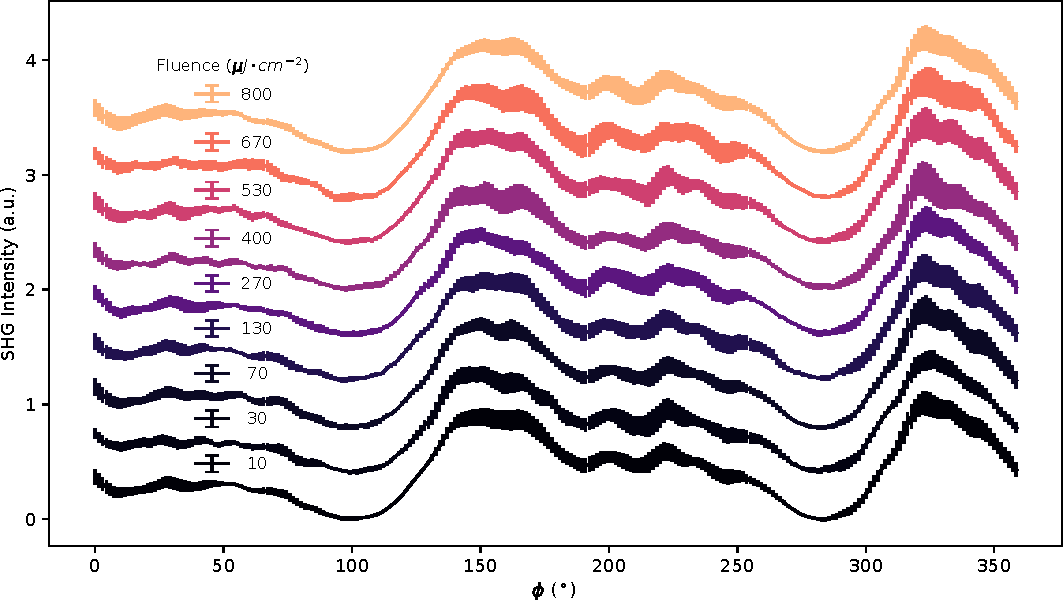
\includegraphics[width=\textwidth]{./gfx/ch6/errorbars.pdf}
\caption{\label{cmb-errorbars}\gls{rashg} results of \cref{cmb-fluencedep} depicted with estimated errorbars (see text).}
\end{figure}

The errorbars in \cref{cmb-errorbars} are ultimately due to uncertainty in the value of the \gls{shg} intensity at each angle $\phi$.
When these angles are integrated over, the associated uncertainties in the \gls{shg} intensity are summed in quadrature.
To extract the uncertainties in the \gls{shg} intensity as a function of angle is a somewhat difficult process, as these uncertainties are largely systematic rather than statistical.
Indeed, the \gls{rashg} pattern should in general be a smooth function of $\phi$; however, it is seen (e.g. \cref{cmb-fig2:d}) that the \gls{rashg} patterns are not necessarily smooth.
We therefore estimate the size of the errorbars using more heuristic methods, which, while imprecise, should at least give a rough approximation to the true uncertainty.

These heuristic errorbars in the \gls{shg} intensity are found by estimating the size of the variations in the \gls{rashg} pattern compared to a smoothed approximation (approximated with an $N=6$ FFT filter).
The errorbars computed this way are shown in \cref{cmb-errorbars}.

\begin{figure}
\centering
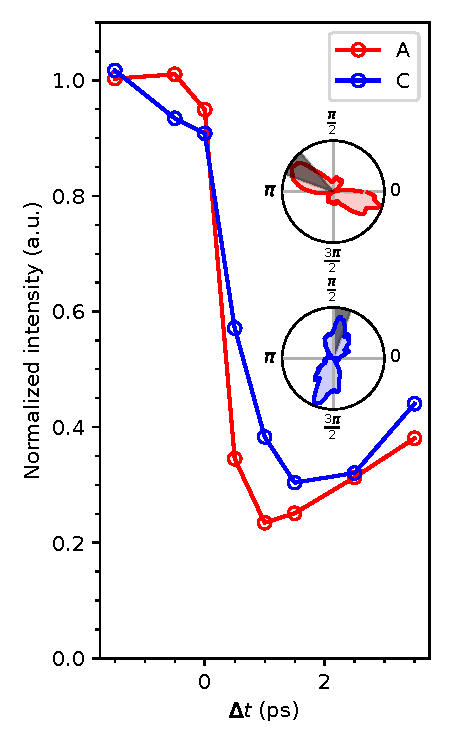
\includegraphics{./gfx/ch6/quenchtimes.pdf}
\captionsetup{singlelinecheck=off}
\caption[Comparison of quench times in different domains]{
\label{cmb-quenchtimes}
Integrated \gls{shg} intensity as a function of time corresponding to \cref{cmb-fig3:a} (A, red) and \cref{cmb-fig3:c} (C, blue).
Insets show the equilibrium \gls{shg} patterns in the \PP polarization combination for the two domains, with the integration region indicated in gray.
The $y$-axis normalization for either domain is defined such that the average signal before zero delay equal to $1.0$.
}
\end{figure}

\begin{figure}
\centering{
\phantomsubfloat{\label{cmb-fluencedep:a}}
\phantomsubfloat{\label{cmb-fluencedep:b}}
}
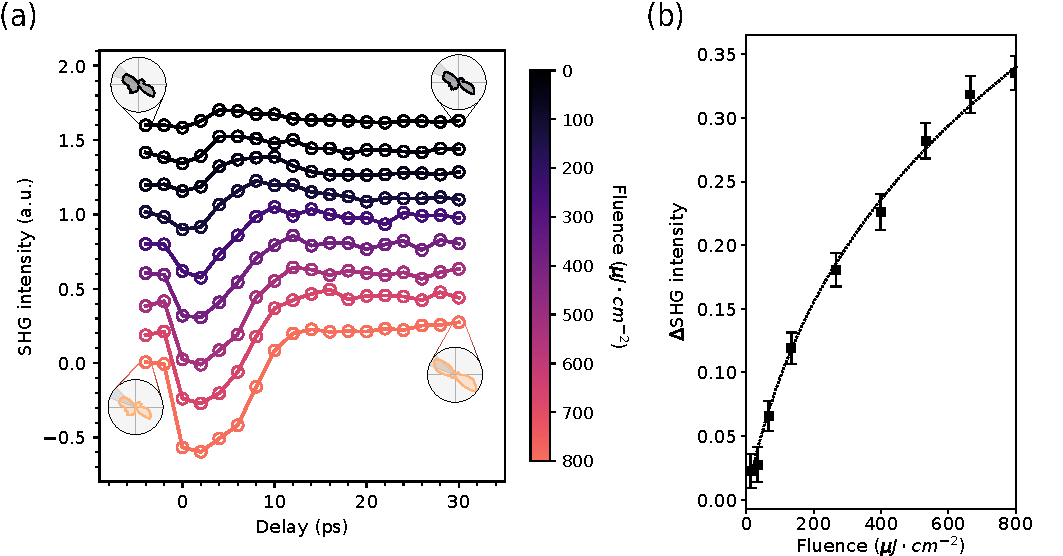
\includegraphics[width=\textwidth]{./gfx/ch6/fluencedep.pdf}
\captionsetup{singlelinecheck=off}
\caption[Fluence dependence if \cmb]{
\label{cmb-fluencedep}
\begin{enumerate*}[label=\caplabel, ref=\capref]
\item Integrated SHG intensity for a representative \gls{afm} domain as a function of delay and pump fluence.
Insets show the initial (left) and final (right) states at high (bottom) and low (top) pump fluences, as well as the integration region (indicated by the shaded area).
\item Difference between the intensity of the integration region specified in \ref{cmb-fluencedep:a} at long times (averaged from $\Delta t=40$ to $\Delta t=\qty{50}{ps}$) and the intensity before zero delay (averaged from $\Delta t=\num{-4}$ to $\Delta t=\qty{-2}{ps}$).
Dashed line is a guide to the eye.
\end{enumerate*}
}
\end{figure}

\begin{figure}
\centering
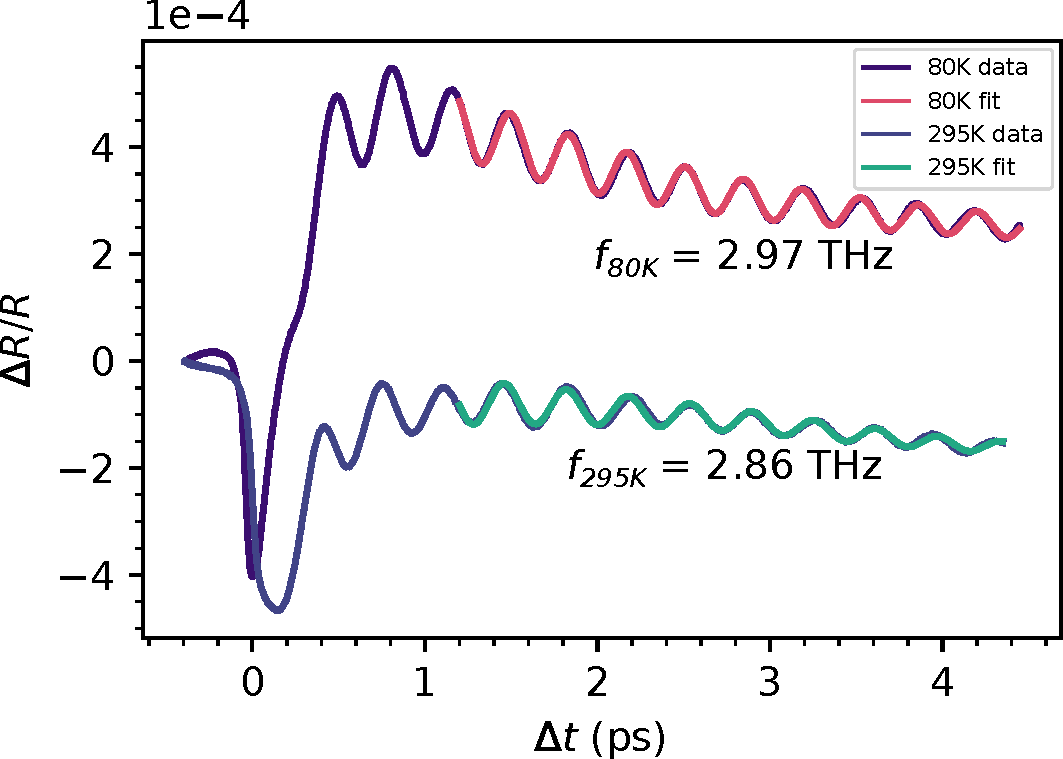
\includegraphics[width=\textwidth]{./gfx/ch6/pp.pdf}
\captionsetup{singlelinecheck=off}
\caption[Pump-probe spectroscopy of \cmb]{
\label{cmb-pp}
Time-resolved reflectivity obtained from \cmb at \qty{80}{K} and \qty{295}{K}.
The pump and probe wavelengths were both \qty{800}{nm}, the pulse width was \qty{28}{fs}, and the pump and probe fluences were \num{10} and \qty{1}{$\mu$ J \cdot cm^{-2}}, respectively.
The data is windowed after the initial transients and then fit to a damped harmonic oscillator plus a polynomial background.
}
\end{figure}

\begin{figure}
\centering
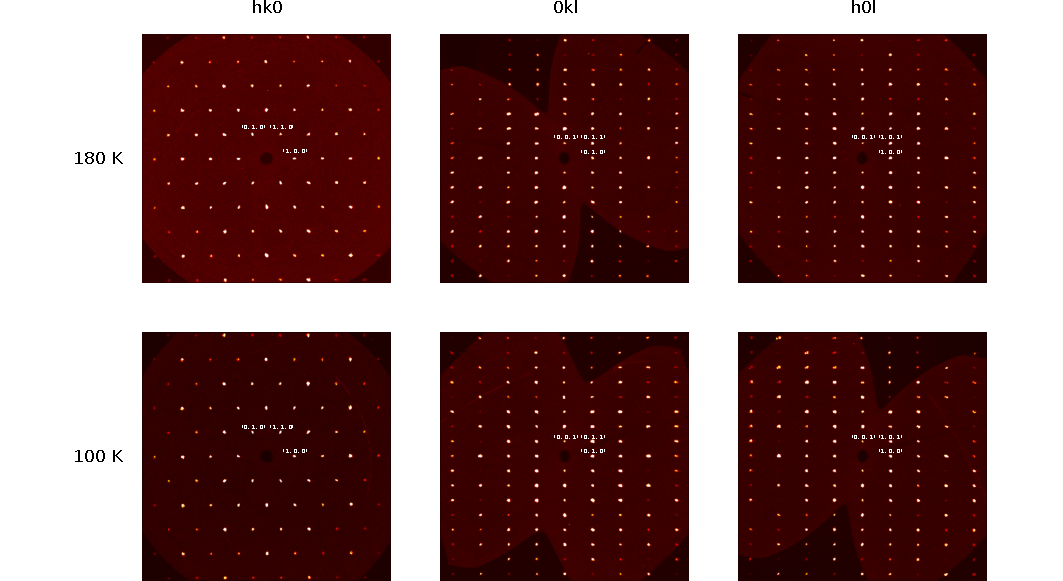
\includegraphics[width=\textwidth]{./gfx/ch6/xrd.pdf}
\captionsetup{singlelinecheck=off}
\caption[\Glsfmtlong{xrd} of \cmb]{
\label{cmb-xrd}
Single-crystal \gls{xrd} precession images obtained from \cmb.
The high temperature refinement is in agreement with previous reports\citep{gibson_magnetic_2015}.
No change in the crystal structure is observed across $T_c=\qty{150}{K}$.
}
\end{figure}

\begin{figure}
\centering
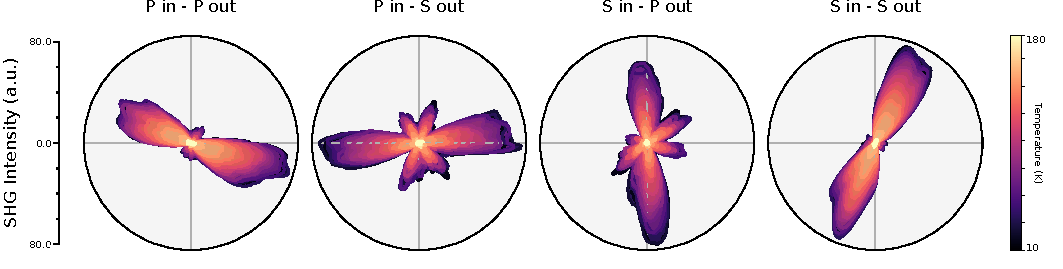
\includegraphics[width=\textwidth]{./gfx/ch6/full_fig0.pdf}
\caption{\label{cmb-fulltempdep}\gls{rashg} results of \cref{cmb-fig0} depicted in all four polarization channels (\PP, \PS, \SP, and \SS)}
\end{figure}

\begin{figure}
\centering{
\phantomsubfloat{\label{cmb-fullequilibrium:a}}
\phantomsubfloat{\label{cmb-fullequilibrium:b}}
\phantomsubfloat{\label{cmb-fullequilibrium:c}}
\phantomsubfloat{\label{cmb-fullequilibrium:d}}
\phantomsubfloat{\label{cmb-fullequilibrium:e}}
}
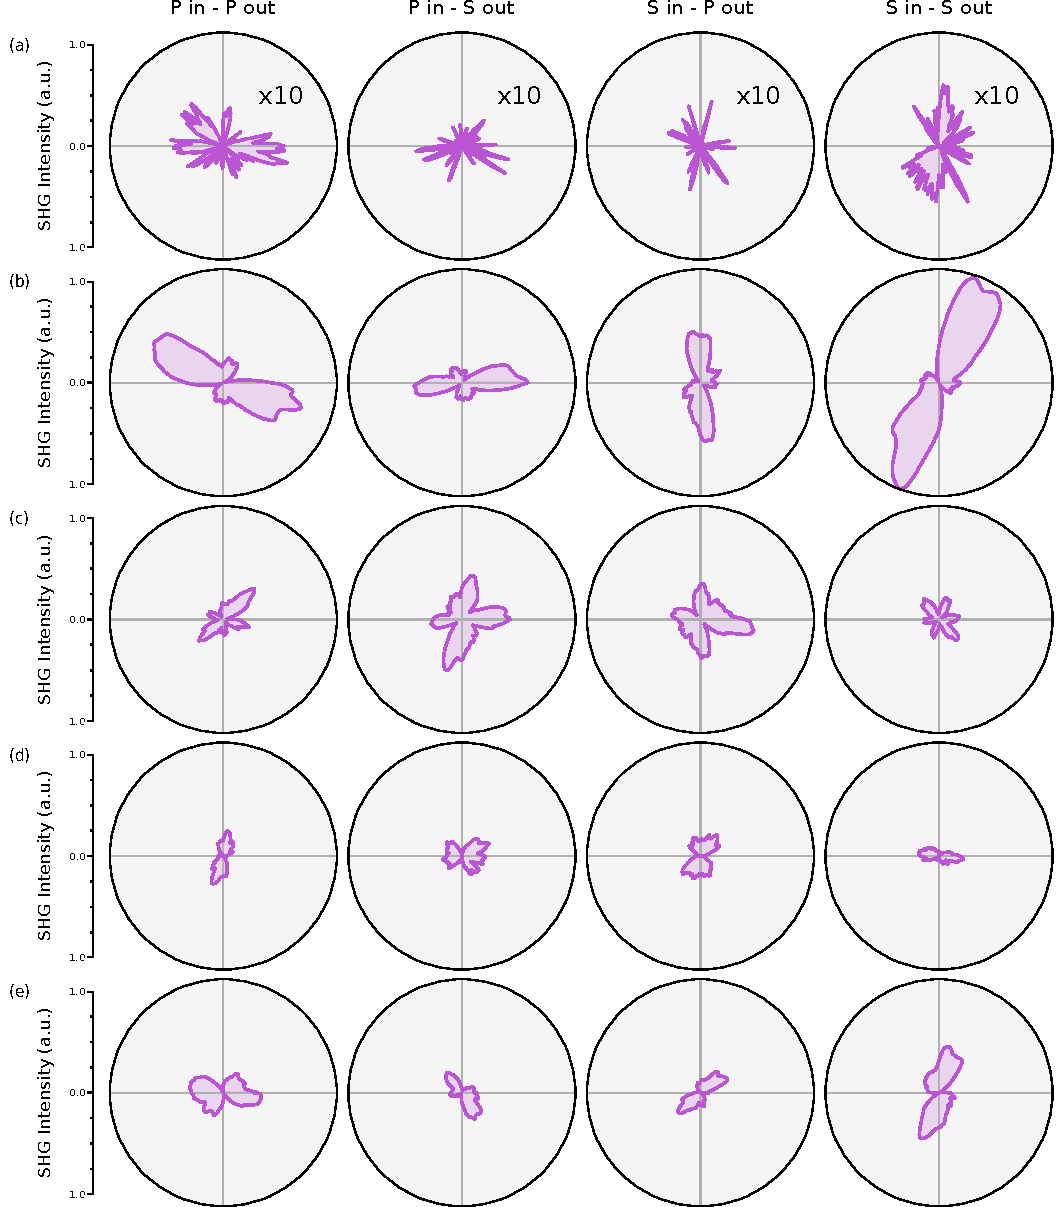
\includegraphics[width=\textwidth]{./gfx/ch6/full_fig1.pdf}
\captionsetup{singlelinecheck=off}
\caption[Full equilibrium \glsfmtshort{rashg} results in \cmb]{
\label{cmb-fullequilibrium}
\begin{enumerate*}[label=\caplabel, ref=\capref]
\item {} \item {} \item {} \item {} \item \gls{rashg} results of \cref{cmb-fig1:b,cmb-fig1:d,cmb-fig1:e,cmb-fig1:f,cmb-fig1:g} depicted in all four polarization channels (\PP, \PS, \SP, and \SS).
\end{enumerate*}
}
\end{figure}

\begin{landscape}
\begin{figure}
\centering
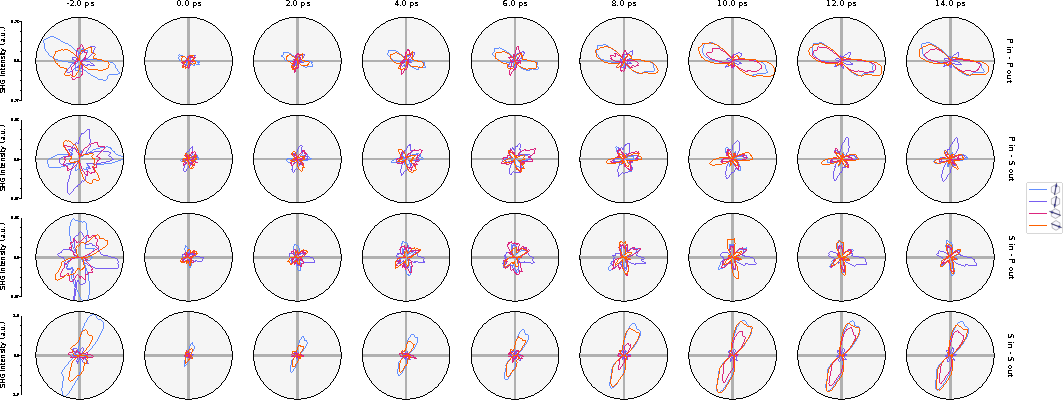
\includegraphics[width=\textwidth]{./gfx/ch6/full_fig2.pdf}
\caption[Full nonequilibrium \glsfmtshort{trshg} results in \cmb]{\label{cmb-fullnonequilibrium}\gls{rashg} results of \cref{cmb-fig2} depicted in all four polarization channels (\PP, \PS, \SP, and \SS).
The pump fluence is set to $\apx \qty{600}{\mu J \cdot cm^{-2}}$.}
\end{figure}
\end{landscape}

\begin{landscape}
\begin{figure}
\centering
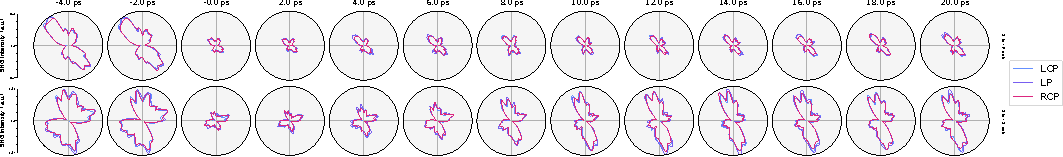
\includegraphics[width=\textwidth]{./gfx/ch6/polarization.pdf}
\caption[Polarization dependence of \glsfmtshort{trshg} results]{\label{cmb-polarization}\gls{rashg} results in a representative domain as a function of time for different pump polarization states (left circularly- (LCP), right circularly- (RCP), and linearly-polarized).
The pump fluence is set to $\apx \qty{600}{\mu J \cdot cm^{-2}}$.
}
\end{figure}
\end{landscape}

\begin{landscape}
\begin{figure}
\centering
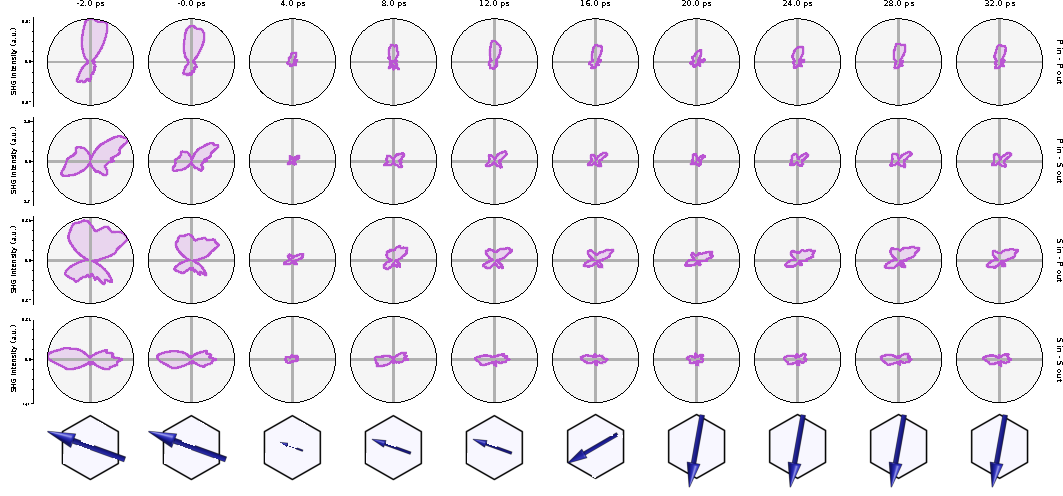
\includegraphics[width=\textwidth]{./gfx/ch6/C2B_short.pdf}
\caption[Transition of \cmb to the state opposite of that presented in the main text]{\label{cmb-CtoBshort}\gls{rashg} snapshots showing a transition to the state opposite to \crefrange{cmb-fig2:c}{cmb-fig2:d}.
The pump fluence is set to $\apx \qty{600}{\mu J \cdot cm^{-2}}$.
\lastrow
The schematic representations beneath the \gls{rashg} plots are for illustration purposes only and the depicted angles are not quantitatively verified.
}
\end{figure}
\end{landscape}

\begin{landscape}
\begin{figure}
\centering
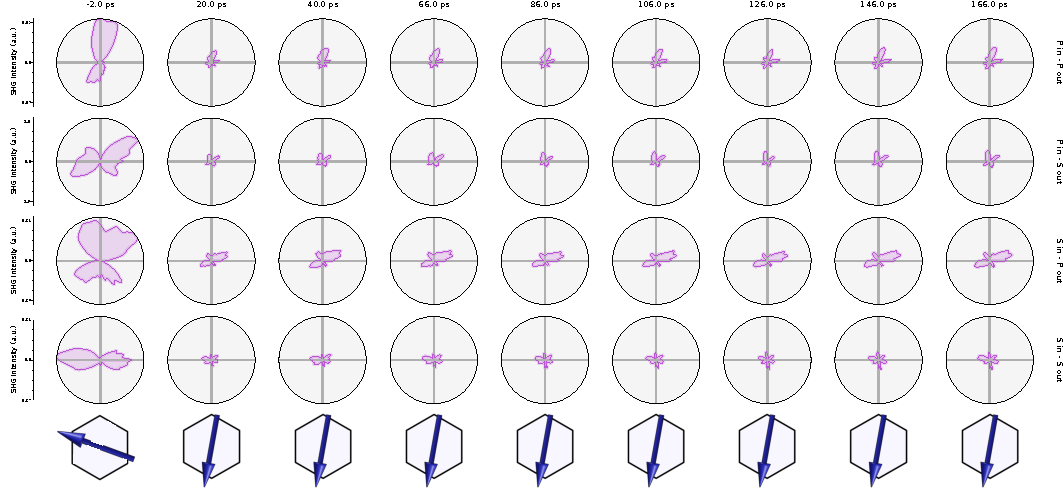
\includegraphics[width=\textwidth]{./gfx/ch6/C2B_long.pdf}
\caption[Transiton of \cmb to state opposite of that presented in the main text, at long times]{\label{cmb-CtoBlong}\gls{rashg} results in the same domain as \cref{cmb-CtoBshort} plotted out to longer times.
The pump fluence is set to $\apx \qty{600}{\mu J \cdot cm^{-2}}$.
\lastrow
The schematic representations beneath the \gls{rashg} plots are for illustration purposes only and the depicted angles are not quantitatively verified.
}
\end{figure}
\end{landscape}

\begin{figure}
\centering
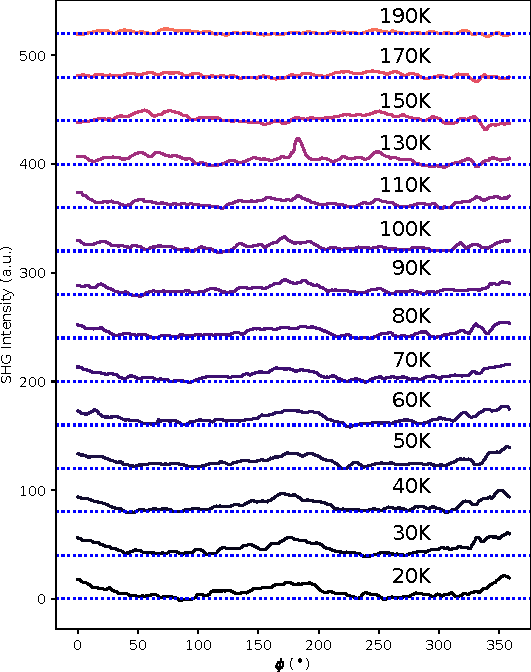
\includegraphics[width=\textwidth]{./gfx/ch6/ctempdep.pdf}
\caption[\Glsfmtshort{shg} intensity in the same domain as \cref{cmb-fig1:f} as a function of temperature]{\label{cmb-ctempdep}
\Glsfmtshort{shg} intensity in the same domain as \cref{cmb-fig1:f} as a function of temperature.
}
\end{figure}

\chapter{Amplitude-mode electromagnon in the spin-spiral multiferroic \ce{CuBr2}}\label{ch:cubr2}
\chaptermark{Amplitude-mode electromagnon in \ce{CuBr2}}
\section{Preface}

This chapter is based on a manuscript intended for standalone publication and modified to fit the format of this thesis.
It was coauthored by myself and Baiqing Lv (as co-first authors), along with Karna Morey, Zongqi Shen, Changmin Lee, Elizabeth Donoway, Alex Liebman-Pel\'{a}ez, Anshul Kogar, Takashi Kurumaji, Martin Rodriguez-Vega, Rodrigo Humberto Aguilera del Toro, Mikel Arruabarrena, Batyr Ilyas, Tianchuang Luo, Peter M\"{u}ller, Aritz Leonardo, Andres Ayuela, Gregory A. Fiete, Joseph G. Checkelsky, Joseph Orenstein, and Nuh Gedik.
It was coauthored by myself, Ajesh Kumar, and Baiqing Lv (as co-first authors), as well as Zongqi Shen, Karna Morey, Qian Song, Riccardo Comin, Todadri Senthil, and Nuh Gedik.
Myself, Baiqing Lv, Zonqi Shen, and Karna Morey took the \gls{trshg} measurements, under the supervision of Nuh Gedik.
Myself and Ajesh Kumar did the theory and analyzed the data, under the supervision of Nuh Gedik and Todadri Senthil.
Qian Song grew the samples, under the supervision of Riccardo Comin.
Myself and Ajesh Kumar wrote the paper, and Nuh Gedik supervised the project.

\section{Abstract}
Below a spontaneous symmetry breaking phase transition, the relevant collective excitations may be described as fluctuations in the amplitude and phase of the order parameter, referred to as \higgs and Goldstone modes, respectively.
In solids, these modes may take on a different character than the equivalent excitations in particle physics due to the diverse vacuum states accessible in condensed matter.
However, the \higgs mode in particular is quite difficult to observe experimentally as it decays quickly into the lower-energy Goldstone bosons and thus has a negligible lifetime in most systems.
In this work, we report evidence for a novel \higgs mode in the multiferroic material \ce{CuBr2}, which shows up as a coherent oscillation in the \glsfmtlong{trshg} signal upon excitation with a femtosecond light pulse.
Since the spiral spin order in \ce{CuBr2} induces a nonzero electric dipole moment in equilibrium, the \higgs mode---which is due to fluctuations in the amplitude of the on-site spin expectation value---is an electromagnon, and thus acquires an inversion quantum number of \num{-1}. 
This is in stark contrast to the \higgs boson of particle physics, which has even parity.
Moreover, the excitation described here represents an entirely new type of electromagnon, distinct from the traditional electromagnon in \glsfmtlong{lswt} which is due to the Goldstone mode.
We argue that the \higgs mode in \ce{CuBr2} acquires a nontrivial lifetime due to the combination of two features: (i) the quasi-\oned nature of the material, and (ii) proximity at zero temperature to a quantum critical point separating the multiferroic ground state from a topological Haldane dimer phase.

\section{Introduction}
When the ground state of a given theory fails to respect one of its symmetries, that symmetry is said to have been be broken spontaneously\citep{durr_zur_1959,nambu_axial_1960}.
The low-energy excitations of this ground state may then be described as excitations of the order parameter either within the subspace of degenerate ground states, or perpendicular to it; these excitations are referred to as Goldstone and \higgs modes, respectively\citep{pekker_amplitudehiggs_2015} (see \cref{cubr2-fig:fig1a}).
This paradigm describes many fundamental phenomena in both particle physics and condensed matter, and the study of these modes has thus emerged as an essential pursuit in both contexts.

\begin{figure}
\centering
\phantomsubfloat{\label{cubr2-fig:fig1a}}
\phantomsubfloat{\label{cubr2-fig:fig1b}}
\phantomsubfloat{\label{cubr2-fig:fig1c}}
\phantomsubfloat{\label{cubr2-fig:fig1d}}
\makebox[\linewidth]{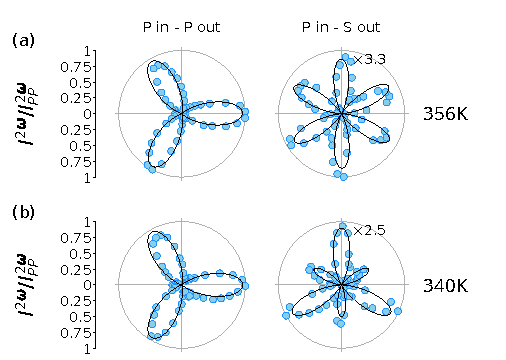
\includegraphics[width=183mm]{./gfx/pdf/fig1.pdf}}
\captionsetup{singlelinecheck=off}
\caption[]{
\label{cubr2-fig:fig1}
\begin{enumerate*}[label=\caplabel, ref=\capref]
\item Mexican hat potential with \higgs and Goldstone modes indicated.
\item $q=0$ electromagnons in the quasi-\oned spin-spiral in the spin (left) and charge (right) sectors.
The \higgs and Goldstone modes are shown in blue and red, respectively.
A second Goldstone mode, corresponding to uniform rotations of the spins about the $z$ axis (which does not affect the polarization $\vec{P}$), is not shown.
\item Magnetic ground state of \ce{CuBr2}.
The macroscopic polarization due to the spin order is depicted with a blue arrow.
The axis labelled $x$ is parallel to the nominal $b$ axis of the crystal structure.
\item Schematic of the \glsfmtshort{trshg} experimental geometry.
\end{enumerate*}
}
\end{figure}

A rich interplay exists between these two fields due to the fact that in particle physics we are limited to a single theory (the standard model), but in condensed matter, the theory is determined by the particular system of interest and may differ dramatically from one material to another.
Thus, various exotic species of \higgs modes may be studied simply by exploring different material systems with spontaneous symmetry breaking.
An important example is in multiferroics, where it has been predicted\citep{matsumoto_electromagnon_2014,matsumoto_electromagnon_2015} that the \higgs mode of the magnetic order (corresponding to modulations in the amplitude of the on-site spin excitation value, see \cref{cubr2-fig:fig1b}) should couple to the macroscopic polarization as an electromagnon, and thus acquire a negative parity eigenvalue.
This is not the case for the Higgs boson of the standard model, which is of even parity\citep{atlas_collaboration_determination_2015}.
In addition to its connection to particle physics, the excitation described here is is also fundamentally different from the traditional electromagnon in multiferroics (which is due to the (pseudo-)Goldstone mode\citep{katsura_dynamical_2007}), and is thus of great interest for magnetoelectric device applications.
Unfortunately, like in particle physics, the \higgs mode in condensed matter is difficult to observe since it may quickly decay into Goldstone bosons upon excitation\cite{jain_higgs_2017}, and the existence of this mode in real multiferroic systems has thus remained an important open question.

In this work, we report evidence for this mode in \ce{CuBr2} (a quasi-\oned, spin-spiral multiferroic, see \cref{cubr2-fig:fig1c}), observed by launching a coherent oscillation of this mode with a near-infrared light pulse and measuring the induced modulations in the electric polarization using a delayed \gls{shg} probe pulse (\cref{cubr2-fig:fig1d}).
We find, as expected, that the mode modulates the macroscopic polarization only along the static ordering direction, and that the frequency of the mode decreases on approaching the critical temperature of the multiferroic order.
These results provide conclusive evidence for the existence of this electromagnon in \ce{CuBr2}, solving a decade-old puzzle and paving the way for future study of the \higgs mode in novel condensed-matter contexts.

\section{Results}
\subsection{Equilibrium}
The low-energy spin Hamiltonian of \ce{CuBr2} is well approximated by the so-called frustrated \oned XXZ spin chain, where localized spin-$1/2$ electrons interact ferromagnetically ($J_1 < 0$) with nearest neighbors but antiferromagnetically ($J_2 > 0$) with next-nearest neighbors (see \cref{cubr2-fig:fig1c}).
When these interaction strengths are of comparable magnitude, the ground state is an incommensurate magnetic spiral, where the ordering wavevector is directed along the chain direction and has the appropriate magnitude so as to balance the two competing interaction terms.
According to theory developed by Katsura, Nagaosa, and Balatsky\cite{katsura_spin_2005}, when spin-orbit coupling is strong this ground state induces an electric polarization at each site $n$ given by
\begin{equation}\label{cubr2-eq:scrosss}
\vec{P}^n \propto \hat{x}\times(\vec{S}^{n} \times \vec{S}^{n+1}),
\end{equation}
where we have set the chain direction to lie along $\hat{x}$.
If the spins lie in the $xy$ plane, then \cref{cubr2-eq:scrosss} induces a macroscopic electric polarization which is equal for each bond and directed purely along the $\hat{y}$ direction (\cref{cubr2-fig:fig1c}).

According to powder neutron diffraction, this spiral magnetic phase is realized in \ce{CuBr2} below $T_c=\qty{75}{K}$ \cite{zhao_cubr2_2012,wang_nmr_2018,zhao_pressure_2019,
zhang_giant_2020}, with the propogation vector (in reciprocal lattice units) given by $\vec{k} = (0, k_y, 0.5)$, with $k_y\sim 0.235$\cite{zhao_cubr2_2012,lee_investigation_2012}.
A pyroelectric current turns on at this temperature as well, indicating a macroscopic electric polarization density $|\vec{P}_0|$ of about \qty{8}{\mu C / m^2} at \qty{10}{K}\cite{zhao_cubr2_2012}.

\begin{figure}
\centering
\phantomsubfloat{\label{cubr2-fig:fig2a}}
\phantomsubfloat{\label{cubr2-fig:fig2b}}
\includegraphics[width=89mm]{./gfx/pdf/fig2.pdf}
\captionsetup{singlelinecheck=off}
\caption[]{
\label{cubr2-fig:fig2}
\begin{enumerate*}[label=\caplabel, ref=\capref]
\item \Gls{shg} intensity as a function of temperature in the \PS polarization channel.
\item Integrated \gls{shg} intensity in the region near $\pi/2$ of \ref{fig:fig2a} marked by the tick marks.
\end{enumerate*}
}
\end{figure}

In a generalized Ginzburg-Landau theory, the \gls{shg} susceptibility tensor $\chi_{ijk}$ is linearly proportional to this polarization:
\begin{equation}\label{cubr2-eq:glshg}
\chi_{ijk}(T<T_c) = \chi_{ijkl}(T>T_c)P_{0l} = \chi_{ijky}(T>T_c)P_0,
\end{equation}
where $\chi_{ijkl}$ is some unknown tensor with the symmetry of the high temperature phase\cite{sa_generalized_2000}, and we have used that $\vec{P}_0 || \hat{y}$.
\cref{cubr2-fig:fig2} shows the temperature dependence of the \gls{shg} intensity in \ce{CuBr2}, indicating a pronounced, order parameter-like enhancement of the \gls{shg} intensity at $T_c$ due to \cref{cubr2-eq:glshg}.
Note that other contributions to the \gls{shg} intensity due to e.g. magnetic dipole, surface electric dipole, and electric quadrupole terms are allowed above and below $T_c$ and thus cannot explain the intensity increase below $T_c$.
In addition, the $c$-type electric dipole term purely due to the magnetic order\cite{birss} is also not allowed by the magnetic point group of the incommensurate spin spiral (see \supcref{sup:magshg}).

\subsection{Nonequilibrium}
\begin{figure}
\centering
\phantomsubfloat{\label{cubr2-fig:fig3a}}
\phantomsubfloat{\label{cubr2-fig:fig3b}}
\phantomsubfloat{\label{cubr2-fig:fig3c}}
\phantomsubfloat{\label{cubr2-fig:fig3d}}
\makebox[\linewidth]{\includegraphics[width=183mm]{./gfx/pdf/fig3.pdf}}
\captionsetup{singlelinecheck=off}
\caption[]{
\label{cubr2-fig:fig3}
\begin{enumerate*}[label=\caplabel, ref=\capref]
\item[] Pump-induced change in the \gls{shg} intensity at \qty{15}{K} in the four polarization channels \item \PP \item \PS \item \SP, and \item \SS.
Insets depict the static \gls{shg} intensity in each polarization channel.
The time-domain signals are computed by performing an azimuthal integration at each delay of the full \gls{shg} pattern over the angles specified by the additional tick marks in each inset.
\end{enumerate*}
}
\end{figure}

Having thus demonstrated that the \gls{shg} intensity is a direct probe of the electric polarization in \ce{CuBr2}, we proceed to investigate the low-energy collective excitations in this phase.
To do so, we excite the sample with a \qty{150}{fs} near-infrared pump pulse, and then probe the \gls{shg} intensity with a second pulse delayed in time by an amount $\Delta t$.
We carry out this procedure in each of four independent polarization channels (\PP, \PS, \SP, and \SS, see \cref{cubr2-sec:methods}), where each channel probes a different linear combination of the tensor elements $\chi_{ijk}$.
The results are shown in \cref{cubr2-fig:fig3}.
Two oscillations, with different dependencies on the \gls{shg} polarization channel, may be observed: one high-frequency mode ($\nu \sim \qty{0.23}{THz}$, $\hbar \omega \sim \qty{1.0}{meV}$), which is only observed in the crossed polarization channels \PS and \SP, and one low-frequency mode ($\nu \sim \qty{0.05}{THz}$, $\hbar \omega \sim \qty{0.20}{meV}$), which occurs in all polarization channels equally.
Both of these are too low to be observed with typical \si{THz} or neutron spectroscopies, yet they are readily apparent in the \gls{trshg} data due to the pump-probe nature of the experiment.

To show that these two modes are directly related to the multiferroic transition at $T_c$, we measure the pump-induced change in the \gls{shg} intensity as a function of $\Delta t$ for a series of temperatures approaching $T_c$ \cref{cubr2-fig:fig4}.
By fitting the respective time-domain traces to damped harmonic oscillators (see \supcref{sup:timedomain}), we can extract the natural frequency of each collective mode as a function of temperature (\cref{cubr2-fig:fig4}).
Both modes exhibit a pronounced softening on approaching $T_c$, confirming their direct involvement in the multiferroic transition.
We also note that both modes disappear above $T_c$, which is sensible given that the macroscopic polarization $\vec{P}_{0}$ also disappears above this temperature.

\begin{figure}
\centering
\phantomsubfloat{\label{cubr2-fig:fig4a}}
\phantomsubfloat{\label{cubr2-fig:fig4b}}
\makebox[\linewidth]{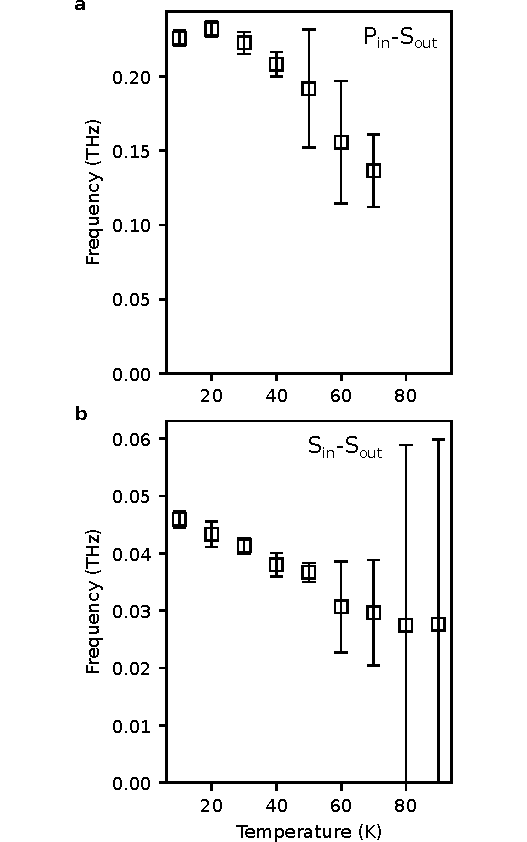
\includegraphics[width=89mm]{./gfx/pdf/fig4.pdf}}
\captionsetup{singlelinecheck=off}
\caption[]{
\label{cubr2-fig:fig4}
\begin{enumerate*}[label=\caplabel, ref=\capref]
\item[] Temperature dependece of the frequencies extracted from the \item \PS and \item \SS time-domain signals (\supcref{sup:timedomain}) in a damped harmonic oscillator model.
Error bars denote \qty{95}{\percent} confidence intervals estimated within a parametric bootstrap (see \supcref{sup:errorbars}).
\end{enumerate*}
}
\end{figure}

To clarify the microscopic origin of these polarization oscillations, we begin by performing \gls{dft}+U and finite-displacement lattice dynamics calculations\cite{} (see \supcref{sup:phonons}) to compare their energies with those of the zone-center phonon modes.
The lowest zone-center optical phonon in this calculation appears at \qty{7.4}{meV}, in excellent agreement with Raman spectroscopy\cite{wang_observation_2017}, and the calculated acoustic phonon branches (which agree with \gls{ins}\cite{wang_observation_2017}) disperse too rapidly to form a zone-folded acoustic phonon mode at the $\Gamma$ point with an energy low enough to match the frequencies observed in the \gls{trshg} experiment.
Thus, the modes observed in \cref{cubr2-fig:fig3,fig:fig4} are not phonons.
The only remaining possibility is that these modes are magnons of the incommensurate spin spiral, which imprint themselves on the polarization via \cref{cubr2-eq:scrosss}; i.e., they are electromagnons.

In \gls{lswt}, there is only one spin boson which couples to the polarization in the spiral magnetic phase of \ce{CuBr2} (see \supcref{sup:pimpliess}); it is the so-called pseudo-goldstone mode of the magnetic order\cite{katsura_dynamical_2007}, which corresponds to a rotation of the spin plane about the chain direction (\cref{cubr2-fig:fig1b}).
This mode has zero energy if the system is isotropic about the chain axis, but in the presence of an anisotropy term it acquires a finite energy.
In \ce{CuBr2}, this energy is expected to lie around \qty{1.25}{meV} (see \supcref{sup:anisotropyenergy}), which is close to the value observed for our high-frequency oscillation (\qty{1.0}{meV}).
Additionally, since this mode involves a rotation of the spin plane about the chain direction, the effect of this mode (from \cref{cubr2-eq:scrosss}) on the polarization is to tilt the vector $\vec{P}_0$ into the $\hat{z}$ direction (\cref{cubr2-fig:fig1b}).
Since the equilibrium polarization lies along $\hat{y}$, \cref{cubr2-eq:glshg} implies that a canting of the polarization $\delta \vec{P} || \hat{z}$ involves new elements of the tensor $\chi_{ijkz}(T>T_c)$ which are not present in equilibrium.
The result is that this mode may appear in different polarization channels with different magnitudes; we thus identify the fast, \qty{0.23}{Thz} oscillation in \cref{cubr2-fig:fig3} with this mode.

The observation of a \emph{second} mode in the \gls{trshg}, however, is impossible to explain in \gls{lswt}, and represents the most striking aspect of this work.
To understand the origin of this second mode, we note that there are only three normal modes of the polarization which occur at the $\Gamma$ point in the Brillouin zone, corresponding to polarization oscillations $\delta\vec{P}$ along $\hat{x}$, $\hat{y}$, and $\hat{z}$.
Since the $\delta\vec{P} || \hat{z}$ mode is already accounted for by the pseudo-goldstone mode, that leaves only $\delta\vec{P} || \hat{x}$ and $\delta\vec{P} || \hat{y}$ as possibilities.
The $\delta\vec{P} || \hat{x}$ mode does not couple to the spin order in this compound\cite{katsura_dynamical_2007}, and in any case is not observable in the geometry of our experiment (see \supcref{sup:nopxmode}).
Thus, the only polarization oscillation which is consistent with the observation of a second mode is an oscillation with $\delta\vec{P} || \hat{y}$.
Since the equilibrium polarization is also directed along $\hat{y}$, this mode simply corresponds to an oscillation in the total amplitude of the polarization, and is thus expected to modulate the overall \gls{shg} intensity irrespective of the polarization channel -- in excellent agreement with \cref{cubr2-fig:fig3}, which shows the low-frequency oscillation appearing in all four polarization channels with equal magnitude.

Naively, electromagnons with $\delta\vec{P} || \hat{y}$ do not exist in \gls{lswt}.
The key insight, however, is that \gls{lswt} neglects dynamics associated with the magnitude of the onsite spin expectation value.
By \cref{cubr2-eq:scrosss}, such dynamics change the magnitude of the induced polarization only, not its direction; i.e., they induce oscillations $\delta\vec{P} || \hat{y}$.
In fact, it is possible to show (see \supcref{sup:pimpliess}) that oscillations along $\hat{y}$ of the induced polarization \emph{necessarily} involve modulations in the amplitude of the onsite spin excpectation value; that is, the only mode which couples to $\delta\vec{P} || \hat{y}$ is the \higgs mode of the magnetic spiral.
Naturally, this mode should soften on approaching $T_c$, in agreement with \cref{cubr2-fig:fig4}.
The \qty{0.05}{THz} oscillation observed in our experiment (which is of similar energy to the \higgs mode in non-ferroelectric quantum magnets\citet{hong_higgs_2017}) is therefore direct evidence for this mode in \ce{CuBr2}, with the additional information that it couples to the electric polarization (i.e., it is an electromagnon) via \cref{cubr2-eq:scrosss}.

\section{Discussion}
Let us make two important remarks about this mode in \ce{CuBr2}.
First, we note that this mode is fundamentally distinct from the \higgs mode in non-multiferroic magnets -- since the multiferroic order breaks inversion symmetry, the \higgs mode of this phase has a parity quantum number $l=-1$ rather than $+1$.
The static polarization $\vec{P}_0$ which appears at $T_c$ can thus be viewed as arising from the odd-parity nature of its \higgs mode.
Second, we remark that the \higgs mode in \ce{CuBr2} can in principle decay -- as in non-multiferroic magnets -- quite rapidly into the Goldstone modes of the magnetic order (which in the spin-spiral phase of \cref{cubr2-fig:fig1c} are gapless and correspond to uniform rotations of each spin about the $\hat{z}$ direction), and thus should not exist as a well-defined quasiparticle unless these decay channels are quenched by some mechanism.

In non-multiferroic magnets, two such mechanisms have been identified.
First, the \higgs mode may be stabilized by bringing the system close to a \gls{qcp}\cite{ruegg_quantum_2008,jain_higgs_2017,hong_higgs_2017,su_stable_2020}, which suppresses the Goldstone bosons and thus stabilizes the \higgs mode.
A second option is to lower the dimensionality\cite{canali_theory_1992,affleck_longitudinal_1992,schulz_dynamics_1996,essler_quasi-one-dimensional_1997,zhou_amplitude_2021}; in \oned, enhanced fluctuations weaken the long range magnetic order and also reduce the spectral weight of the Goldstone bosons\cite{zhou_amplitude_2021}. 
In \ce{CuBr2}, not only is the system fundamentally one-dimensional, but is thought also to lie in close proximity to a zero-temperature \gls{qcp}\cite{furukawa_ground-state_2012} separating the spiral phase considered here and a paraelectric Haldane dimer phase.
Both of these mechanisms thus likely contribute to stabilizing the \higgs electromagnon in \ce{CuBr2}.

\section{Conclusion}
To summarize, we have presented evidence of a novel electromagnon arising from the \higgs mode of the spiral magnetic order in \ce{CuBr2}.
This mode appears alongside the pseudo-Goldstone mode in the \gls{trshg} data as a low-frequency oscillation in the longitudinal component of the electric polarization, which softens on warming close to $T_c$.
Looking forward, we note that the two mechanisms we identified for stabilizing this mode in \ce{CuBr2} -- low dimensionality and potential proximity to a \gls{qcp} -- are not necessarily unique to this material.
Thus, the \higgs electromagnon presented here may in fact be a common feature of \oned multiferroics, and its observation could indicate a wealth of new opportunities to explore the \higgs mode of particle physics in novel condensed-matter contexts.

\section{Methods}\label{cubr2-sec:methods}
\Gls{trshg} measurements were carried out using a fast-rotating optical grating setup described previously\citep{fichera_second_2020,harter_high-speed_2015,torchinsky_low_2014}.
\qty{100}{fs} ultrashort pulses from a regeneratively amplified \qty{5}{kHz} \ce{Ti}:Sapphire laser were used to pump an \gls{opa}, producing \qty{1300}{nm} (\cref{cubr2-fig:fig3}) or \qty{1650}{nm} (\cref{cubr2-fig:fig4}) pump pulses which were delayed with an optical delay line and focused at normal incidence to a \qty{300}{um}-diameter spot on the sample.
The pump fluence was $\sim \qty{1}{mJ\cdot cm^{-2}}$ for all measurements.
A small portion of the \ce{Ti}:Sapphire output was used for the \gls{shg} probe experiment, the output of which was spectrally filtered with a \qty{400}{nm} bandpass filter, collected by a photomultiplier tube, filtered with a lock-in amplifier, and correlated with the plane of incidence angle using an optical rotary encoder.
To measure the pump-induced change in the \gls{shg} signal, the pump pulses were chopped at a frequency of \qty{2.5}{kHz}, and the lock-in amplifier was set to that frequency so as to measure $I_{\mathrm{pump}+\mathrm{probe}}-I_\mathrm{probe}$.
For the pump-probe \gls{rashg} measurements, the plane of incidence was rotated while the delay stage was moved and the polarizers were controlled automatically using homebuilt polarization rotators described in \citet{morey_automated_2024}.
For the single-angle \gls{trshg} measurements, the plane of incidence was parked at the angle which maximized the static \gls{shg} intensity in the respective polarization channel.

\section{Supplementary material}

\subsection{Electromagnons in \ce{CuBr2}}\label{cubr2-sup:pimpliess}
The observed co-existence of spiral magnetic order and ferroelectricity is due to the spin-orbit coupling enabled interaction term between the spins $\vec S$ and the electronic polarization $\vec P$~\cite{}:
\begin{equation}
    H_{s-P} = \lambda \sum_i \vec P_i \cdot (\hat x \times \vec S_i \times \vec S_{i+1})
\end{equation}
The ordered state for $T<T_N$ is a multiferroic with spontaneous polarization
\begin{equation}
\left<\vec P_i\right> = P_0 \hat y
\end{equation}
and spiral spin ordering
\begin{equation}
\left< \vec S_i\right> \equiv \vec S_{0,i} = S_0 \left( \cos (\vec Q \cdot \vec R_i) \hat x + \sin (\vec Q \cdot \vec R_i) \hat y\right),
\end{equation}
where $\vec Q$ is the spin-ordering wavevector and $\vec R_i$ are the spatial coordinates of the Cu atoms.
Let us consider fluctuations about this ordered state and ask which fluctuations are detectable via SHG.
Representing fluctuations in the polarization by $\delta \vec P_i$ and spin by $\delta \vec S_i$, we get the following fluctuation Hamiltonian:
\begin{equation}\label{cubr2-eq:fluctuationhamiltonian}
    H^f_{s-P} = \lambda \sum_i \delta \vec P_i \cdot (\hat x \times \delta \vec S_i \times \vec S_{0,i+1} + \hat x \times \vec S_{0,i} \times \delta \vec S_{i+1}) + \mathcal{O}(\delta \vec P^2, \delta \vec S^2).
\end{equation}
Expanding the spin fluctuations along all directions, we find that they couple only to polarization fluctuations along $\hat y$ and $\hat z$.
Focusing on zero-momentum polarization fluctuations (since they are sensitive to SHG),
\begin{equation}\label{cubr2-eq:ftfluctuationhamiltonian}
\begin{aligned}
H^f_{s-P} = &i \sin (\vec Q \cdot \vec a) \delta P_z(\vec q=0) \left(\delta S_z(-\vec Q) - \delta S_z (\vec Q) \right)\\
&+\sin (\vec Q \cdot \vec a) \delta P_y(\vec q=0) \left( -\delta S_x(-\vec Q) + i\delta S_y(-\vec Q) - \delta S_x(\vec Q) - i\delta S_y(\vec Q) \right)\\
& + \mathcal{O}(\delta \vec P^2, \delta \vec S^2)
\end{aligned}
\end{equation}
where $\vec a$ is the lattice vector along the chain.
Transverse polarization fluctuations $\delta P \sim \hat z$ couple to a uniform rotation of the spin-plane about the $x$ axis.
These are the electromagnons discussed in \citet{katsura_dynamical_2007}.
The longitudinal fluctuations, on the other hand, couple to longitudinal fluctuations of the magnetization on each site.

\subsection{Energy of the pseudo-Goldstone mode}\label{cubr2-sup:anisotropyenergy}
An expression for the frequency of the pseudo-Goldstone mode in the presence of an easy-plane anisotropy is given by \citet{katsura_dynamical_2007} as
\begin{equation}
\omega_- = \sqrt{A(Q)B(Q)},
\end{equation}
where
\begin{align}
A(q) &= 2S\left[\frac{2J(Q)-J(Q+q)-J(Q-q)}{2}\right],\\
B(q) &= 2S\left[J(Q)-J(q)+D\right],\\
J(q) &= 2\left[J_1\cos(qa)+J_2\cos(2qa)\right],
\end{align}
$D$ is the anisotropy energy, and $2S$ is the amplitude of the spin in units of $\mu_B$.

Using $Q=\qty{0.235}{rlu}$\citep{zhao_cubr2_2012}, $J_1=\qty{8.8}{meV}$\citep{lebernegg_magnetism_2013}, $J_2=\qty{-22.2}{meV}$\citep{lebernegg_magnetism_2013}, $D=\qty{0.15}{meV/\ce{Cu}}$\citep{lee_investigation_2012}, and $2S=\num{0.38}$\citep{lee_investigation_2012}), we have
\begin{equation}
\omega_- = \qty{1.3}{meV}
\end{equation}
in good agreement with the experiment.

\subsection{Fits of time domain signals}\label{cubr2-sup:timedomain}
Time-domain plots corresponding to the frequencies in \cref{cubr2-fig:fig4} are illustrated in \cref{cubr2-fig:timedomain}.
Each plot is a least-squares fit of the data to a damped harmonic oscillator model
\begin{equation}
I^\mathrm{SHG}_p(t, \params) = P^0_p\delta P_p(t, \params)+[\delta P_p(t)]^2,
\end{equation}
where
\begin{equation}\label{cubr2-eq:model}
\delta P_p = A_pe^{-\gamma_p t}\cos\left(\sqrt{(2\pi\nu_p)^2-\gamma_p^2}t+\psi_p\right),
\end{equation}
$p \in \{\mathPS, \mathSS\}$, and $\params$ denotes the set of free parameters to be estimated.

The main conclusion of these fits is that the frequency of the two modes (most notably, the low-frequency \SS mode) soften on approaching $T_c$.
This may also be seen heuristically from the time-domain signals without doing any fits.
\cref{cubr2-fig:timedomain_zoom} shows an enlarged (i.e., scaled to account for the decrease in signal amplitude) view of the \SS signal for three temperatures below $T_c$, showing a clear decrease in the oscillation frequency at high temperature.
\cref{cubr2-fig:timedomain_nosoften} shows an alternative fit where the frequency parameter $\nu_\mathrm{SS}$ is constrained to be constant as a function of temperature, showing that our data is not consistent with a hypothetical model where the frequency shift with temperature in \cref{cubr2-eq:model} is only attributed to the damping term $\gamma_\mathrm{SS}$.

\begin{figure}
\phantomsubfloat{\label{cubr2-fig:timedomaina}}
\phantomsubfloat{\label{cubr2-fig:timedomainb}}
\centering
\makebox[\linewidth]{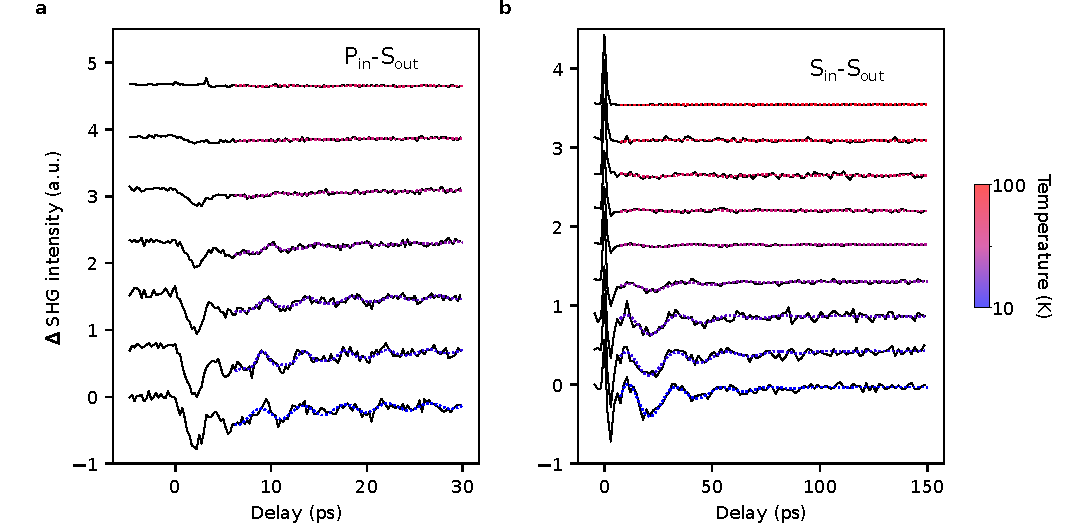
\includegraphics[width=183mm]{./supgfx/pdf/timedomain.pdf}}
\captionsetup{singlelinecheck=off}
\caption[]{
\label{cubr2-fig:timedomain}
\begin{enumerate*}[label=\caplabel, ref=\capref]
\item[] Time-domain signals corresponding to \item \cref{cubr2-fig:fig4a} and \item \cref{cubr2-fig:fig4b}.
Dashed lines depict least-squares fits to the data in a damped harmonic oscillator model, see \supcref{sup:timedomain}.
\end{enumerate*}
}
\end{figure}

\begin{figure}
\centering
\makebox[\linewidth]{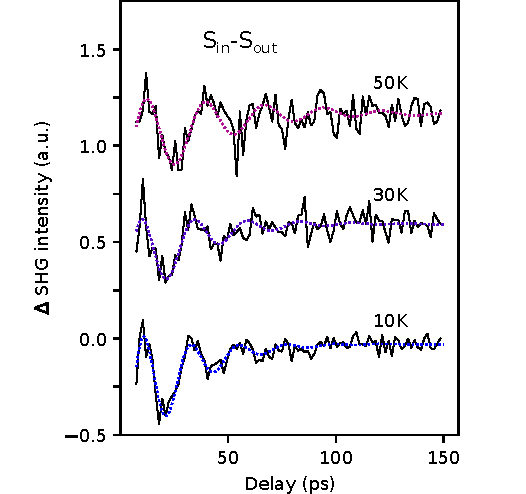
\includegraphics[width=89mm]{./supgfx/pdf/timedomain_zoom.pdf}}
\captionsetup{singlelinecheck=off}
\caption[]{
\label{cubr2-fig:timedomain_zoom}
\begin{enumerate*}[label=\caplabel, ref=\capref]
\item[] Rescaled \SS time-domain signals (see \cref{cubr2-fig:timedomainb}) for select temperatures below $T_c$.
\end{enumerate*}
}
\end{figure}

\begin{figure}
\centering
\makebox[\linewidth]{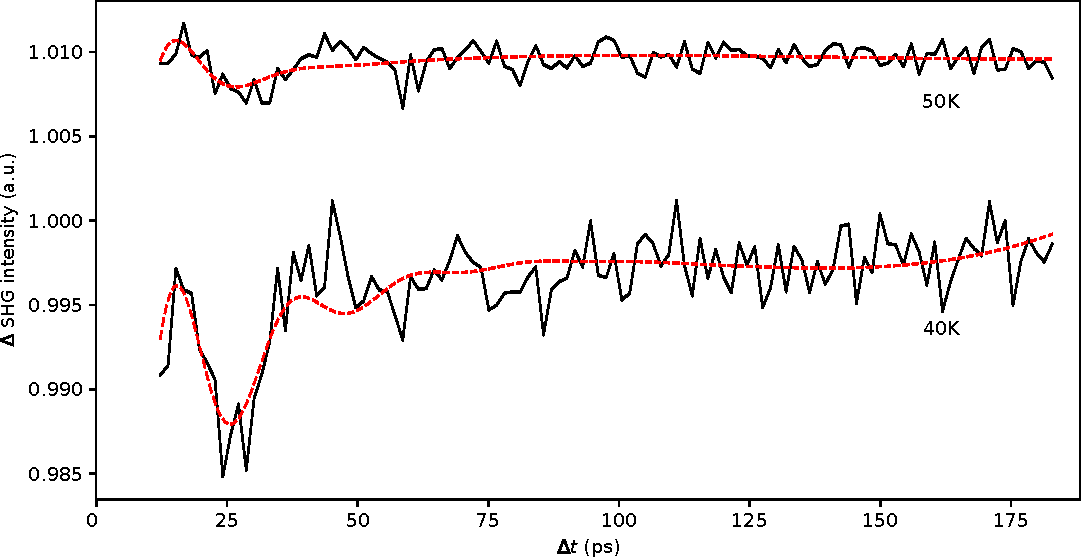
\includegraphics[width=183mm]{./supgfx/pdf/timedomain_nosoften.pdf}}
\captionsetup{singlelinecheck=off}
\caption[]{
\label{cubr2-fig:timedomain_nosoften}
\begin{enumerate*}[label=\caplabel, ref=\capref]
\item[] \SS time-domain signals (see \cref{cubr2-fig:timedomainb}) for select temperatures approaching $T_c$.
Dashed lines depict least-squares fits to the data in a variant of \cref{cubr2-eq:model} where $\nu_\mathrm{SS}$ is constrained not to vary with temperature.
\end{enumerate*}
}
\end{figure}

\subsection{Error bars in \cref{cubr2-fig:fig4}}\label{cubr2-sup:errorbars}
In this section, we describe how the uncertainties in the least square estimates of the frequency parameter $\nu$ of \cref{cubr2-eq:model}, which are depicted as a function of temperature in \cref{cubr2-fig:fig4}, were calculated from the the time-domain signals in \cref{cubr2-fig:timedomain}.
For each temperature and polarization channel, a \gls{lm} algorithm was used to find the minimum $\params_0$ of the objective function
\begin{equation}\label{cubr2-eq:objectivefunction}
f_p(\theta) \propto \sum_{n=0}^{N-1}\left(I^\mathrm{SHG}_p(t_n, \params) - I^\mathrm{SHG}_{p,n}\right)^2,
\end{equation}
where $\{(t_n, I^\mathrm{SHG}_{p,n}), n\in (0, 1, \ldots, N-1)\}$ are the data points in \cref{cubr2-fig:timedomain}, and we have assumed the noise level is independent of delay.
The uncertainty in each parameter is estimated within a parametric bootstrap\citep{dekking}: for each temperature, \num{1000} bootstrap samples are generated by adding noise (normally distributed, with variance given by the variance of data points at long times where the signal is constant) to the \gls{lm} estimate $I^\mathrm{SHG}_p(t_n, \params_0)$.
For each bootstrap sample $s$, an estimate $\params_s$ is computed by minimizing \cref{cubr2-eq:objectivefunction} as above, and the \qty{95}{\percent} confidence interval reported in \cref{cubr2-fig:fig4} is taken to be \num{1.96} times the standard deviation of the distribution $\{\params_s-\theta_0\}$.

\subsection{Fits to static RASHG data}\label{cubr2-sup:static}
The static \gls{shg} intensity was fit by \cref{cubr2-eq:shgintensityequation}.
The susceptibility tensor was taken to be the form \cref{cubr2-eq:susceptibilityshortform}, plus an additional $C_1$ component (likely due to surface adsorbates).
The result is shown in \cref{cubr2-fig:static}.

\begin{figure}
\centering
\makebox[\linewidth]{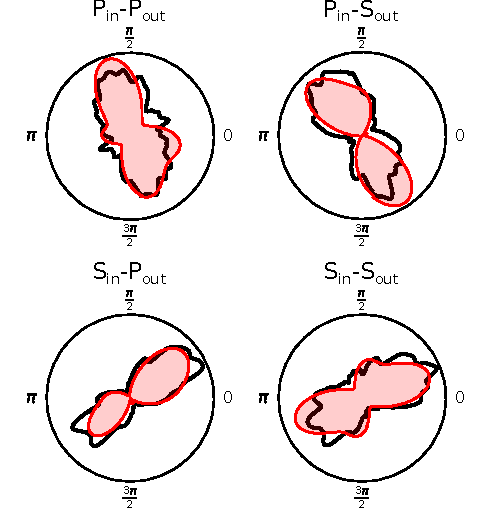
\includegraphics[width=89mm]{./supgfx/pdf/static.pdf}}
\captionsetup{singlelinecheck=off}
\caption[]{
\label{cubr2-fig:static}
\begin{enumerate*}[label=\caplabel, ref=\capref]
\item[] Fits (red) to static \gls{rashg} data (black) depicted in \cref{cubr2-fig:fig3}.
\end{enumerate*}
}
\end{figure}

\subsection{Excluded possibilities for observed results}\label{cubr2-sup:excluded}
\subsubsection{$\delta \vec{P} || \hat{x}$ oscillation\label{cubr2-sup:nopxmode}}

Without loss of generality, let the maximum of the SHG in \SP occur when the incoming electric field is along $\hat{x}$.
Then, we have:
\begin{equation}
\Delta I_\mathrm{SP}^\mathrm{SHG} \propto |\hat{e}^\mathrm{out}_i \chi_{ijkl}\hat{e}^\mathrm{in}_j\hat{e}^\mathrm{in}_k[P_{0l}+\delta P_l]|^2-|\hat{e}^\mathrm{out}_i \chi_{ijkl}\hat{e}^\mathrm{in}_j\hat{e}^\mathrm{in}_kP_{0l}|^2
\end{equation}
with $\hat{e}^\mathrm{in}_i || x$ and $P_{0l} || y$, we have
\begin{equation}
\label{cubr2-eq:longdeltai}
\Delta I_\mathrm{SHG} \propto 2\hat{e}^\mathrm{out}_i \hat{e}^\mathrm{out}_j\chi_{ixxy} \chi_{jxxx}P_{0y}\delta P_x + \hat{e}^\mathrm{out}_i \hat{e}^\mathrm{out}_j\chi_{ixxx} \chi_{jxxx}\delta P_x\delta P_x 
\end{equation}
Since we are in \SP, $\hat{e}^\mathrm{out}_i \perp x$; thus, \cref{cubr2-eq:longdeltai} involves the tensor elements $\chi_{yxxx}$ and $\chi_{zxxx}$.
Both of these elements are zero due to the $x \rightarrow -x$ mirror symmetry.
Thus, the $\delta \vec{P} || \hat{x}$ oscillation is not visible in our experiment.

Additionally, since the $\delta \vec{P} || \hat{x}$ mode does not couple to the spin order in this compound\cite{katsura_dynamical_2007}, its frequency should be far above the frequencies observed in our experiment (which are determined by the energy scales of the spin Hamiltonian).

\subsubsection{Zone-folded acoustic phonons}\label{cubr2-sup:phonons}

Phonon band structure calculations were carried out using the finite displacement method\citep{togo_first_2015} with a distance of \qty{0.01}{\angstrom} within a $3\times3\times3$ supercell.
Forces were calculated via the DFT-D2 method\cite{grimme_semiempirical_2006} and LDA+U method\cite{dudarev_electron-energy-loss_1998} ($U_\mathrm{\ce{Cu}}=\qty{3}{eV}$) using a $7\times7\times5$ $k$-mesh with \num{122} irreducible $k$-points and a plane-wave cutoff energy of \qty{100}{eV}.
The result is shown in \cref{cubr2-fig:phonons}.
The acoustic phonons in \cref{cubr2-fig:phonons} all disperse too rapidly for the \qty{0.05}{THz} oscillation in the \gls{trshg} to be consistent with a zone-folded (at $k=(0, 0.235, 0.5)$) acoustic phonon.

\begin{figure}
\centering
\makebox[\linewidth]{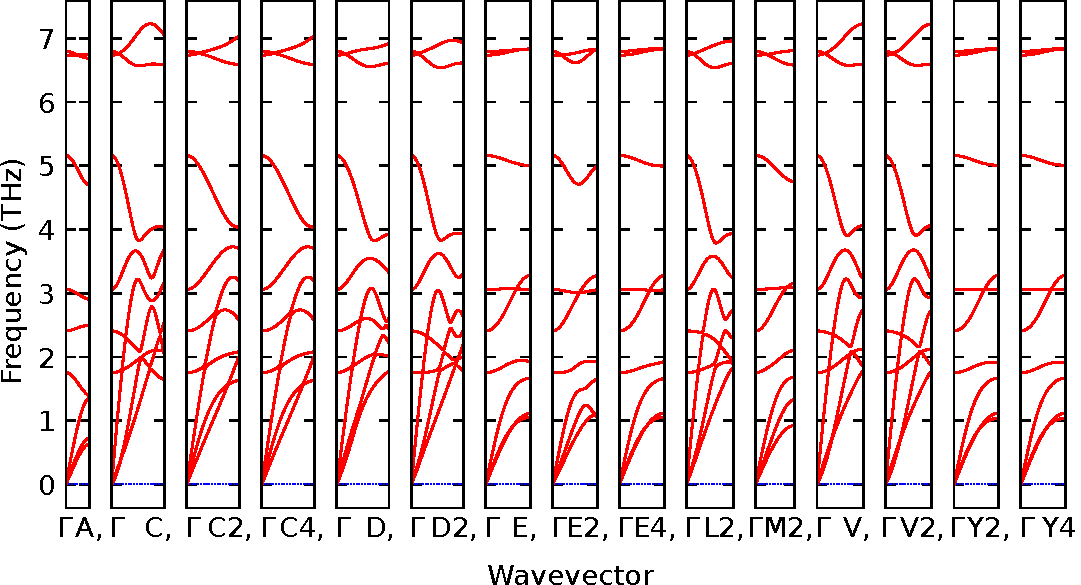
\includegraphics[width=183mm]{./supgfx/pdf/phonons.pdf}}
\captionsetup{singlelinecheck=off}
\caption[]{
\label{cubr2-fig:phonons}
\begin{enumerate*}[label=\caplabel, ref=\capref]
\item[] Phonon band structure of \ce{CuBr2} within a finite displacement calculation.
\end{enumerate*}
}
\end{figure}

\subsubsection{Magnetic SHG}\label{cubr2-sup:magshg}

In principle, magnetic systems with broken inversion symmetry may generate electric-dipole SHG with or without a static electric dipole moment.
In this section, we wish to show that this is not the case in \ce{CuBr2}; i.e., in \ce{CuBr2}, the SHG intensity is a direct measure of the macroscopic electric dipole moment.

Indeed, in the presence of such a static electric dipole moment $\vec{P}_0$, we typically expect the SHG response to be directly proportional to it; i.e.
\begin{equation}\label{cubr2-eq:shgintensityequation}
I(2\omega) \propto |\hat{e}^\mathrm{out}_i \chi_{ijk} \hat{e}^\mathrm{in}_j \hat{e}^\mathrm{in}_k|^2,
\end{equation}
where
\begin{equation}\label{cubr2-eq:susceptibilityshortform}
\chi_{ijk} = \chi_{ijkl} P_{0l},
\end{equation}
and $\hat{e}^\mathrm{in}$, $\hat{e}^\mathrm{out}$ are unit vectors in the direction of the incoming and outgoing electric fields, respectively.
In \ce{CuBr2}, we have  
\begin{equation}
\vec{P}_0 = \sum\limits_{\left<i, j\right>} \hat{x} \times \vec{S}_i \times \vec{S}_j,
\end{equation}
i.e., the static polarization is quadratic in the spin degree of freedom.

The question, then, is whether there exists some additional term
\begin{equation}
\chi'_{ijk} = \chi_{ijkl} G_{0l},
\end{equation}
where $\vec{G}_0$ is either (a) linear in spin, or (b) quadratic in the spins but not of the form $\sum_{\left<ij\right>}\vec{S}_i\times\vec{S}_j$.
For case (b), note that the term $\sum_{\left<ij\right>}\vec{S}_i\times\vec{S}_j$ is the only quadratic form which is simultaneously antisymmetric in the bond direction and $\vec{q}=0$ (i.e. each bond has the same coefficient).

For case (a), we argue here that any such term is weak due to the approximate time-reversal symmetry of the spiral magnetic order.
Consider first a four-site commensurate approximant of the incommensurate spin spiral.
This phase has a symmetry element consisting of the time-reversal operation followed by a translation by half of the magnetic supercell.
Thus, the point group contains time-reversal symmetry.
Since $\vec{G}_0$ is linear in spin, time-reversal takes $\vec{G}_0\rightarrow-\vec{G}_0$; but since time-reversal is a symmetry, it must also take $\chi'_{ijk}\rightarrow\chi'_{ijk}$ and $\chi_{ijkl}\rightarrow\chi_{ijkl}$.
Thus, $\chi'_{ijk}=0$ in the commensurate approximation.

In the incommensurate case, note that the magnetic point group of an incommensurate magnetic phase is defined as the set of point-group operations present in the operations belonging to the superspace group.
Thus, for a single-k incommensurate magnetic structure, time-reversal is always an element of the magnetic point group.
This is due to the fact that the lattice constant in the chain direction is $3.51$ \si{\angstrom}, so lengthscales associated with translations in the space group are much smaller than the probe wavelength ($\sim\qty{800}{nm}$).
The symmetry group ``seen'' by the probe thus contains time reversal to a very good approximation.

\subsubsection{Multi-phason excitation}

While the amplitude mode of the spin spiral in \ce{CuBr2} is the only single-particle excitation which couples to $\delta P_y$ (see \cref{cubr2-eq:ftfluctuationhamiltonian}), in principle multiparticle excitations consisting of, e.g., two phasons with opposite momenta are also allowed.
However, note that the relevant energy scale which defines the phason sound velocity depends on the intra-chain coupling terms, which are $\bigO(\qty{10}{meV})$; the peak in the phason joint density of states thus occurs at this high energy scale, which is much larger than the \qty{0.2}{meV} energy of our low-frequency oscillation.
Multi-phason excitations are thus not consistent with the long-lived oscillation observed in our experiment.

\chapter{Concluding remarks}\label{ch:conclusion}
We began this thesis by discussing how strong interactions may invalidate the Fermi liquid model and result in novel quantum ground states which are not possible to understand within a single-particle picture.
The result is a situation where there is no general theory at present capable of predicting, \textit{a priori}, the ground state and low-energy excitations of an arbitrary correlated quantum material.
We have obviously not come any closer to such a theory over the course of this research---although, in truth, that was never really the goal.
What we have done instead is to enlarge our inventory of novel phenomena which can occur in quantum materials (acknowledging, of course, that specifying such an inventory is essential for solving the correlated electron problem), and in this sense we have met some success.
Using a novel experimental technique (\gls{trshg}), we showed that antiferromagnets may be manipulated nonthermally by quenching the equilibrium order on ultrafast timescales, in a fashion which is similar in spirit to previous works on \gls{cdw} systems \citep{fausti_light-induced_2011,kogar_light-induced_2020}.
We also showed that spin-spiral multiferroic materials may host novel electromagnon excitations which are due not to the pseudo-Goldstone mode, but to the amplitude mode of the magnetic order.
Both of these discoveries were quite unexpected, and each of them \emph{required} measuring the full \gls{rashg} signal at each time delay---a technology that was developed (partially by us) only over the course of the last \num{10}--\num{15} years.
The story, then, is that a new technique was developed, and then that technique led us to new physics that we didn't previously know existed.

This story is quite common in condensed matter physics.
Consider, for example, the discovery of antiferromagnetism, which is no doubt more common in solids than ferromagnetism.
Nevertheless, ferromagnetism induces a net magnetic dipole moment, and the resulting macroscopic magnetic properties are thought to have been understood by humans as early as the fourth millenium B.C. \citep{magnetism_fundamentals}.
Antiferromagnets, in contrast, took until the \nth{20} century to be predicted \citep{neel_properties_1948} and experimentally discovered \citep{shull_neutron_1951}---the latter required the development of neutron scattering.
Thus, new techniques which are sensitive to different order parameters or excitations very often lead to new discoveries in condensed matter physics.

In light of this history, in my view there is no reason to think that the technology we have at present is sufficient to solve the correlated electron problem.
This is a perspective which is often voiced in the context of \ce{URu2Si2}, a heavy-fermion material with a phase transition at \qty{17.5}{K} to an ordered state whose order parameter and low-energy excitations remain unknown despite nearly thirty years of investigation \citep{palstra_superconducting_1985}.
It is thought \citep{alexandradinata_future_2022} that the puzzle has remained unsolved simply because we do not, at present, have an experimental probe which couples to the order in this compound.
Going forward, I thus predict that technique development will be the fundamental driving force for progress in strongly correlated electron physics.
A large part of this will involve \emph{improving} techniques that we already have (using, for example, machine learning, or \nth{4}-generation synchrotron sources) to increase signal-to-noise, ease of data processing, etc.
A parallel effort will be to imagine totally different experimental probes (such as, for example, scattering of entangled particles\citep{shen_unveiling_2020}), although this is obviously more difficult.

There is potentially some criticism to be made of the \emph{approach} we take to the correlated electron problem in present era of modern science.
At the time of writing, a large portion of the research which is published in high-impact factor journals in this field is of the type pursued in this thesis---systematic research is largely \emph{avoided} in favor of surprising or unexpected results, which are, in the most pessimistic view, easier for journals to shape into a headline.
My feelings on this issue are somewhat mixed.
In the worst case, the current research climate deters researchers from pursuing systematic research, on the basis that it is more difficult to publish.
At the same time, the field is still somewhat in its infancy, and I do think that there are a large number of fundamental phenomena in quantum materials that simply have yet to be discovered.
Perhaps, then, the right research to be doing is indeed more exploratory right now than would otherwise feel comfortable.

In either case, I \emph{am} sure that there is \emph{absolutely no reason} to be publishing in for-profit journals!
Perhaps this would be understandable if the for-profit journals offered a monetary incentive to authors who elect to publish there.
But the reality is the opposite---in the publishing industry, the \emph{suppliers} pay for the goods that they provide, and then pay again to consume those goods.
This bizarre circumstance is possible only because of a valuation heuristic (which occurs at all levels of academic discourse---from faculty hiring decisions to grad lounge chit-chat) that ranks papers on the basis of which journal they are published in.
This results in a situation where the publishing industry itself holds all of the power in directing what scientists decide to study; thus the conventional wisdom that one should avoid manganites and cuprates since these are not of interest to editors of high-impact factor journals.
This is, in my opinion, the biggest impediment to progress right now in correlated electron physics.

One immediate solution would be the adoption of, for example, a ``journal of null or uninteresting results'', where authors could receive citations for research which is not flashy but may nevertheless be useful.
In the long term, however, the field must transition away from the for-profit publication industry, which may involve the difficult task of redefining our research valuation metholodgy.
To some extent I think this is already happening; many of the graduate students and postdocs I talk to share a similar point of view, and after all, those are the people that will eventually be making decisions about who gets tenure at academic institutions.

In any case, the idea that the correlated electron problem is important---something which I hope to have reinforced through the research conducted in this thesis---is certainly not something that will go away.
There is thus a bright future ahead for this field, and I am quite confident in the condensed matter community to help make that future a reality.


\backmatter*
\bibliography{fichera-bfichera-phd-physics-2024-source}

\end{document}
